\documentclass[12pt]{report}

% install / use required packages
\usepackage[a4paper, left=1in, right=1in, bottom=1in, top=1in]{geometry}
\usepackage{nomencl}
\usepackage{array}
\usepackage{mathtools}
\usepackage{nicefrac}
\usepackage{float}
\usepackage{subcaption}
\usepackage{adjustbox}
\usepackage{multirow,tabularx,booktabs}
\usepackage{setspace}
\usepackage{titlesec}
\usepackage{tocloft}

\usepackage[hidelinks]{hyperref}
\usepackage[acronym]{glossaries}

\usepackage{bookmark}

\usepackage{tikz}
\usetikzlibrary{shapes.geometric,arrows,calc}

\usepackage{caption}
\captionsetup{justification=raggedright,singlelinecheck=false}
\captionsetup[subfigure]{justification=centering}

\usepackage{graphicx}
\graphicspath{{./images/}}

\makeatletter
% set the default path to search for input latex files
\def\input@path{{./content/}}
\makeatother

\makeglossaries

\newglossarystyle{mylong} {
\setglossarystyle{long}

\renewenvironment{theglossary}
    {\begin{longtable}[l]{@{}p{\dimexpr 4cm-\tabcolsep}p{0.8\hsize}}}
    {\end{longtable}}
    
\renewcommand{\glossentry}[2] {
    \glsentryitem{##1}\glstarget{##1}{\glossentryname{##1}} &
    \Glossentrydesc{##1}
    \tabularnewline}
}

\setglossarystyle{mylong}

\newacronym{afff}{AFFF}{aqueous film-forming foam}
\newacronym{faa}{FAA}{Federal Aviation Administration}
\newacronym{naa}{NAA}{National Aviation Authority}
\newacronym{nfpa}{NFPA}{National Fire Protection Association}
\newacronym{fp}{FP}{fluoro protein foam}
\newacronym{fffp}{FFFP}{film-forming fluoro protein foam}
\newacronym{ar-afff}{AR-AFFF}{alcohol-resistant aqueous film-forming foam}
\newacronym{ar-afffp}{AR-AFFFP}{alcohol-resistant film-forming fluoro protein foam}
\newacronym{jp-4}{JP-4}{jet propellant}
\newacronym{ph}{Ph}{potential for hydrogen}
\newacronym{ahj}{AHJ}{authority having jurisdiction}
\newacronym{caa}{CAA}{civil aviation authorities}
\newacronym{icao}{ICAO}{international civil aviation authority}
\newacronym{caf}{CAF}{compressed air foam}
\newacronym{nrcc}{NRCC}{National Research Centre of Canada}
\newacronym{ndt}{NDT}{non-destructive testing}
\newacronym{lldpe}{LLDPE}{linear low-density polyethylene}
\newacronym{fcc}{FCC}{face centred cubic}
\newacronym{hcp}{HCP}{hexagonal closed pack}
\newacronym{bcc}{BCC}{body centred cubic}
\newacronym{osha}{OSHA}{Occupational Safety and Health Act}
\newacronym{saiw}{SAIW}{The Southern African Institute of Welding}
\newacronym{fea}{FEA}{finite element analysis}
\newacronym{acsa}{ACSA}{Airports Company South Africa}
\newacronym{cr}{Cr}{chromium}
\newacronym{ni}{Ni}{nickel}
\newacronym{mo}{Mo}{molybdenum}
\newacronym{hsla}{HSLA}{high-strength low-alloy steel}
\newacronym{he}{HE}{hydrogen embrittlement}
\newacronym{rh}{RH}{relative humidity}
\newacronym{micat}{MICAT}{The Ibero-American Map of Atmospheric Corrosiveness}
\newacronym{osd}{OSD}{On-site Stormwater Detention}
\newacronym{un/ece}{UN/ECE}{United Nations Economic Commission for Europe}
\newacronym{tow}{TOW}{time of wetness}
\newacronym{iso}{ISO}{International Standardization Organization}
\newacronym{tem}{TEM}{transmission electron microscopy}
\newacronym{pe}{PE}{polyethylene}
\newacronym{ldpe}{LDPE}{low-density polyethylene}
\newacronym{mdpe}{MDPE}{medium-density polyethylene}
\newacronym{hdpe}{HDPE}{high-density polyethylene}
\newacronym{xlpe}{XLPE}{cross-linked polyethylene}
\newacronym{icp-aes}{ICP-AES}{inductively coupled plasma atomic emission spectroscopy}
\newacronym{ftir}{FTIR}{Fourier transform infrared spectroscopy}
\newacronym{dls}{DLS}{dynamic light scattering}
\newacronym{icp}{ICP}{inductively coupled plasma}

\glsaddallunused

\setcounter{secnumdepth}{4}
\setlength{\parindent}{0pt}

% TODO: space out tables
% TODO: Fix declaration page
% TODO: Fix bookmark locations

% change the title of the table of contents
\renewcommand*\contentsname{Table of Contents}

% change the title of the bibliography
\renewcommand*\bibname{References}

% change the line spacing inside tables
\renewcommand{\arraystretch}{1.5}

\newcommand{\phantomaddcontentsline}[3] {
    \phantomsection
    \addcontentsline{#1}{#2}{#3}
}

% ensures that words aren't hyphenated when the word is at the end of a line.
% \tolerance=1
% \emergencystretch=\maxdimen
% \hyphenpenalty=10000
% \hbadness=10000

\begin{document}
% change the margins around chapter title for the entire document.
\titlespacing*{\chapter}{0pt}{-25pt}{20pt}

\begin{titlepage}
\begin{center}

%\doublespacing
%\vspace*{1cm}

\renewcommand{\baselinestretch}{1.2}

{\Large\bf
The Impact of The Storage Facility on Performance\\[6pt] Parameters of Aqueous Film-Forming Fire-Fighting\\[12pt] Foam (AFFF) in Aviation Fire Protection}

\vspace{10mm}


\includegraphics[width=0.6\textwidth]{images/logo.png}

\vskip 10mm

\Large
\textbf{Nhlanhla Fortune Khanyi} \\

\vspace{40mm}

\large
Submitted in fulfilment of the academic\\
requirements for the degree of

\vspace{4mm}

MASTER OF ENGINEERING \\
in MECHANICAL ENGINEERING 

\vspace{4mm}

in the \\
Department of Mechanical Engineering \\
Durban University of Technology



\vspace{\stretch{1}}
\normalsize
Durban \\
2023

\end{center}
\end{titlepage}

% \cleardoublepage
\pagenumbering{roman}

% change the chapter title format for the first section of the document.
\titleformat{\chapter}{\normalfont\Large\bfseries}{}{0em}{}

\onehalfspacing
\section*{Declaration}
\addcontentsline{toc}{chapter}{\bf Declaration}


I, \textbf{Nhlanhla Fortune Khanyi}, declare that:   

\begin{enumerate}
    \item The research reported in this thesis, except where otherwise indicated, is my original research. 
    \item The thesis has not been submitted for any degree or examination at any other university. 
    \item This thesis does not contain other persons' data, pictures, graphs, or other information unless specially acknowledged as being sourced from other persons.  
    \item This thesis does not contain other persons' writing unless specially acknowledged as being sourced from other researchers. Where other written sources have been quoted, then:  
    
    \begin{enumerate}
        \item Their words have been rewritten, but the general information attributed to them has been referenced.  
        \item Where their exact words have been used, then their writing has been placed in italics and inside quotation marks and referenced.  
    \end{enumerate} 
    
    \item This thesis does not contain text, graphics, or tables copied and pasted from the internet unless specially acknowledged, and the source is detailed in the thesis and the reference sections. 
\end{enumerate}

\vskip 5mm

{\bf Student:}  \makebox[44mm]{\hrulefill}\hfill \makebox[40mm]{\hrulefill}\\
{\bf Nhlanhla F Khanyi} \hfill Date



\section*{Acknowledgements}
\addcontentsline{toc}{chapter}{\bf Acknowledgements}

I would like to express my sincere gratitude to the following people for their assistance, guidance, and support during this study:

\begin{itemize}
    \item My supervisor, Prof. P, Y. Tabakov for his continual guidance, advice, and mentorship throughout my research. His patience with my endless queries, extensive knowledge of engineering studies, and enthusiasm for the whole project were great motivations, and I am very thankful to him.

    \item My former colleague, Mapule Molabe for her continual assistance from the commencement of this report. You know this thesis would have not even started without your technical expertise, and for that I thank you.  

    \item My friend, Andile Ntanjana for his continual assistance in reviewing my report regularly and providing technical expertise was necessary.

    \item My friend, Yamkelani Mlunguza for her continual assistance in reviewing my report and guiding me in the right direction throughout the years. 

    \item I would also like to extend my sincere gratitude to my family members and my dearest friends for their unwavering support throughout my degree study.
    
    \item Special gratitude goes to National Research Foundation (NRF) for their funding (reference \textbf{MND200611530513}). It also brings me great pleasure to convey my appreciation to Columbus Stainless (Pty) Ltd for supplying the duplex stainless steel for experimental purposes. Lastly, the Durban University of Technology (DUT) for assisting with \acrshort{ftir} and \acrshort{dls} instruments.
 \end{itemize}
\chapter{Abstract}
Aqueous Film Forming Foam (AFFF) has become a critical constituent within the aviation industry. It was declared by National Fire Protection Association (NFPA) as a sole optimum extinguishing agent for suppression of hydrocarbon fires. Nevertheless, unexpected circumstances occur when AFFF is unable to perform as anticipated. In the aviation industry, this is normally noticed during periodic tests. As a consequence, it has become a necessity to monitor the performance of AFFF on a regular basis.
The aim of this study is to investigate the impact of the storage facility on the performance parameters of AFFF. The principal focus is on the materials that are commonly used to construct the storage tanks used for storing AFFF concentrate, namely mild steel, stainless steel, and high-density polyethylene (HDPE). The aim focuses specifically on ascertaining if these materials affect the properties of AFFF concentrate, thus influencing its performance during firefighting. In this way, it is uncomplicated to explore materials that are innocuous to AFFF concentrate. Furthermore, the optimization of these materials in such a way that they are compatible with AFFF concentrate becomes a feasible alternative.
A qualitative research approach was used to investigate the impact of the materials used to construct the storage tank for storing AFFF concentrate. Based on the aforementioned challenges, Fourier transform infrared spectroscopy (FTIR), transmission electron microscopy (TEM), dynamic light scattering, and inductively coupled plasma atomic emission spectroscopy (ICP-AES) were all used for testing the materials. The findings from the primary research concluded that the three materials affect the foaming ability and foam stability of the AFFF solution, with the severity being the variance. HDPE was found to have a less severe impact, while stainless steel had a tolerable impact. The findings demonstrated that mild steel greatly affects the aforementioned performance parameters of AFFF. Based on these findings, it was concluded that mild steel is incompatible with AFFF concentrate.
The study was limited to the effects of the materials on any AFFF performance parameters. Consequently, the study recommends that mild steel should be heat treated to enhance its properties in such a way that it is innocuous to AFFF concentrate. The study further recommends that other materials, such as fiber glass and cross-linked polyethylene (XLPE), be established as potential materials for constructing AFFF storage facilities.
\chapter{Dedication}


\doublespacing

\tableofcontents

\clearpage
\phantomaddcontentsline{toc}{chapter}{List of figures}
{\renewcommand{\numberline}[1]{Figure #1:~}
\listoffigures}

\clearpage
\phantomaddcontentsline{toc}{chapter}{List of tables}
{\renewcommand{\numberline}[1]{Table #1:~}
\listoftables}

\phantomaddcontentsline{toc}{chapter}{Nomenclature}
\printnomenclature

\phantomaddcontentsline{toc}{chapter}{List of acronyms}
\printglossary[title=List of acronyms, type=\acronymtype, nonumberlist]

% reset the chapter numbering
\setcounter{chapter}{0}
% \cleardoublepage
\pagenumbering{arabic}

% change the chapter title format for the entire document.
\titleformat{\chapter}{\normalfont\Large\bfseries}{\chaptertitlename\ \thechapter:}{0.5em}{}

\onehalfspacing
\chapter{Introduction}
\section{Introduction}
This chapter provides an overview of the content structure of the study and the background of the issues underlying this study. The research objectives are comprehensively stated in accordance with the research outputs the study seeks to achieve. The motivations behind the present study are clearly stated. Moreover, an overview of the format/layout of the entire dissertation is briefly discussed, and the content of the following chapter is stated.

\section{Background to the Problem}
Fire protection is a critical sector within any aviation industry, which has created divergent opinions in terms of compliance standards. Aircraft accidents are devastating, considering the loss of lives and costly equipment that must be expected. In aviation, firefighting foam, particularly \acrfull{afff}, is the sole optimum extinguishing agent for suppression of combustible or flammable liquids. As a matter of fact, in South Africa, aviation accidents involving aircraft have dramatically decreased over the past decades. Nonetheless, it is obligatory for the aviation industry to adhere to the relevant compliance standards and be fully equipped in case of any unexpected circumstances.

Periodic training is mandatory in all aspects of aviation fire protection in ensuring that firefighting skills and resources within the sector adhere to the \acrfull{faa}, \acrfull{naa}, and \Acrfull{nfpa} compliance standards, to react rapidly during accidents. Consequently, periodic testing of the performance parameters of fire extinguishing foam is a necessity. Unexpected circumstances often happen during periodic tests when \acrshort{afff} is unable to perform as anticipated. The main priority of \acrshort{afff} is to suppress the fire and allow possible victims more time to escape during the accident. However, according to relevant compliance standards, all of this must be accomplished in one minute or less upon arrival at the accident scene. The poor performance of \acrshort{afff} is caused by numerous and diverse factors; hence, it becomes difficult to examine where the problem originates.

\section{Significance of the Study}
In past decades, there have been fatal fire accidents in the aviation industry, which has tasked researchers to investigate further on the fire protection sector. Nevertheless, there are still notable gaps in previous research conducted, with limited studies on the impact of the storage tank of the firefighting foams. This is due to the nature and diversity of these problems. The complexity of focusing on the optimization of firefighting foam in the storage facility has always been a concern due to the complicated branches of engineering such as material sciences, structural analysis, and thermal engineering involved. 

In 1965, Meldrum et al. \cite{meldrum1965storage} published their study on the storage life and utility of mechanical firefighting foam liquids. The study contributed to predicting the period in which firefighting foams can be held in a storage facility before they deteriorate. Furthermore, it emphasized the gaps and limitations within previous research and the difficulties in problem optimization. The predictions are governed by parameters such as extreme temperatures, oxidation, evaporation, corrosion, dilution, and contamination on the storage facility. Most of this research work will be benchmarked by \cite{meldrum1965storage}. Extensive research on the impact the storage facility or tank has on \acrshort{afff} will be conducted.

This research work has great significance in terms of evaluating the impact of storage facilities on \acrshort{afff} performance, which is also dependent on a number of factors that have been aforementioned. All manufacturers of firefighting foam concentrate have strict recommendations for storing their products, with the priority being to store the foam concentrate in its original storage tank. The challenge arises due to critical factors that must be taken into consideration and often result in large storage tanks being constructed on-site. The large storage facilities are beneficial as foam concentrate can be pumped rapidly from one source to firefighting vehicles during emergency conditions without the huge demand for replenishment. Consequently, these critical considerations lead to storing firefighting foam concentrate in different storage tanks rather than the original, recommended containers.

\section{Objectives and Methodology}
Motivated by these challenges, the purpose of the present research work is to experimentally evaluate and assess the impact of the storage facility on any performance parameters of \acrshort{afff}. The study examines the compatibility of engineering materials, namely mild steel, stainless steel, and \acrfull{hdpe}. These are the materials that are commonly used when constructing a storage facility for firefighting foam concentrate, specifically \acrshort{afff}. This is accomplished by performing several analyses that evaluate the effect of each material on the \acrshort{afff} concentrate and, thus, on the performance parameters. In all these analyses, the pure \acrshort{afff} concentrate is utilized as a benchmark to deduce any vital alterations. In such a manner, it is possible to enhance the properties of these engineering materials based on the heat treatment process, microstructural analysis, and environmental stress cracking in such a way that they are compatible with \acrshort{afff} concentrate. All these optimization methods aim to effectively store \acrshort{afff} concentrate without affecting its performance parameters or chemical composition during vital fire accidents.

\section{Scope}
The scope of this study is limited in the following regards: Firstly, the study is only concerned with the effect of the materials on \acrshort{afff} concentrate. It does not investigate the causes of these effects, but this can be accomplished in future research. Secondly, the study does not practically test the performance of \acrshort{afff}, as would normally happen in the aviation industry during periodic tests or aircraft accidents. Rather, the study experimentally assesses the properties of \acrshort{afff} concentrate and then draws scientific conclusions based on the relevant literature.

\section{Thesis layout}
The study consists of six chapters structured as follows:

\subparagraph*{Chapter 1: Introduction}\hfill\\
This chapter provides a brief overview of the organisation included in the study as well as the background to the problem underlying the research work. It outlines the aim and importance of the study. It explains the research objectives, formulates the research questions, and discusses the format of the study.

\subparagraph*{Chapter 2: Literature review}\hfill\\
Chapter 2 provides a comprehensive summary of the existing literature on \acrshort{afff} that was consulted. It focuses on the broader knowledge of previous studies that relate to the problems of interest in this study.

\subparagraph*{Chapter 3: Evaluation of materials of construction}\hfill\\
The current and previous studies on the compatibility of engineering materials with \acrshort{afff} concentrate have been conducted. This is then validated by the experimental analysis in Chapter 5 based on the outcomes.

\subparagraph*{Chapter 4: Experimental set up}\hfill\\
The experimental set-up for the tests and analyses that were conducted in this study is documented in this chapter. All the materials and equipment used during the tests are also shown, and their significance is concisely described.

\subparagraph*{Chapter 5: Results and discussion}\hfill\\
This chapter documents and discusses the results from the experimental tests conducted in Chapter 4. The results were recorded and benchmarked with the standard parameters. The conclusions are drawn based on outcomes and the existing literature review. 

\subparagraph*{Chapter 6: Conclusions and further work}\hfill\\
This chapter concludes the study with a summary of research findings aimed at solving the research problem. The scope for future research areas is discussed and the conclusion for the entire study made.

\section{Conclusion}
Considering the devastation caused by hydrocarbon fires, the fire protection sector cannot be overlooked in the aviation industry. This chapter provided a brief overview of the entire study, which included background information on the problem, a statement of the problem, objectives, and the significance of the study. The format of the study was also described. The next chapter explores the literature that is relevant to this study.
\chapter{Literature review}
\section{Introduction}
This chapter aims to provide an overview and foundation of the current knowledge of this study in literature as well as a theoretical base for the work done in this study. Fundamentals pertaining to this study are presented. The solution techniques related to \acrshort{afff} have been proposed and analysed by many researchers. All optimization problems are about maximizing the effectiveness and efficiency of \acrshort{afff}. Inputs and outputs of these solution techniques have different limitations and difficulties which lead researchers to propose ideas about finding the best solution to these techniques.

The first section of the literature is a brief overview of significant fundamentals of \acrshort{afff}-focusing on the evolutionary changes, characterization, foaming ability, mechanical stability, and critical application rates. This is followed by a review and analysis of current problems and difficulties based on the optimization of \acrshort{afff}. Issues concerning the compatibility of various storage facilities on \acrshort{afff} are discussed. Previous studies and experimental work aiming at the optimization of \acrshort{afff} are discussed.

\section{A brief overview of various firefighting foams}
In the aviation industry, fire is of great concern due to the incidences of fires that are usually devastating to both human lives and properties. Since fire is of great significant in the present research, it is beneficial to understand various classes of fire. Fire is usually classified in five (5) classes. In fire science, fire is classified by the type of fuel they burn namely: Class A, B, C, D, and K. \cite{oguike2013study}.  The classes are discussed in detail in Table \ref{ch2:table:classes}. However, the present research work will only focus on Class B fire, since \acrshort{afff} is utilised to suppress this Class of fire.

\begin{table}[H]
\onehalfspacing
\centering
\caption{Various classes of fire \cite{hinnant2020characterizing}.}
\begin{tabularx}{\textwidth}{ >{\hsize=.45\hsize}X >{\hsize=1.35\hsize}X >{\hsize=.9\hsize}X }
\hline
Class of fire & Type of fire & Commonly encountered \\ 
\hline
A & Common combustibles such as wood, paper, and rubber materials. & General places. \\
B & Flammable liquids such as fuel, petroleum greases, and flammable gases. & Airports and petroleum industries. \\
C & Energized electrical equipment and conductors. & Electrical distribution industries. \\
D & Combustible metals such as magnesium, titanium, and sodium. & Metal manufacturers. \\ 
K & Cooking oils, normal grease, and animal fat. & Production and FMCG industries. \\
\hline
\end{tabularx}
\label{ch2:table:classes}
\end{table}

In the aviation industry, firefighting foam was declared by \acrshort{faa} as the sole optimal extinguishing medium used for suppression of Class B fire during emergency conditions. Originally, five types of firefighting foams are commonly used: \acrfullpl{fp}, \acrfullpl{afff}, \acrfullpl{fffp}, \acrfullpl{ar-afff} and \acrfullpl{ar-afffp} \cite{george2002introduction}. All of them were designed to be effective in handling precise fire conditions and contain one or more fluorinated surfactants as a key ingredient.

In general, foam is made by first mixing foam concentrate with water to create a foam solution. This aqueous solution is then blended with air using standard aspirating nozzles to generate foam \cite{george2002introduction}.  Fire-fighting foam is an extinguishing agent composed of numerous bubbles formed mechanically or chemically from the liquid, as shown in Figure \ref{ch2:figure:scheme}. These are commonly used to reduce the spread and extinguishing of Class B fires and to prevent re-ignition whilst in certain situations may be implemented to extinguishing Class A fires \cite{oguike2013study}. Sometimes capabilities of firefighting foams can be reduced due to ignorance. Hence foam may be assumed to have performance concerns, whereas it does not. 

\begin{figure}[H]
    \centering
    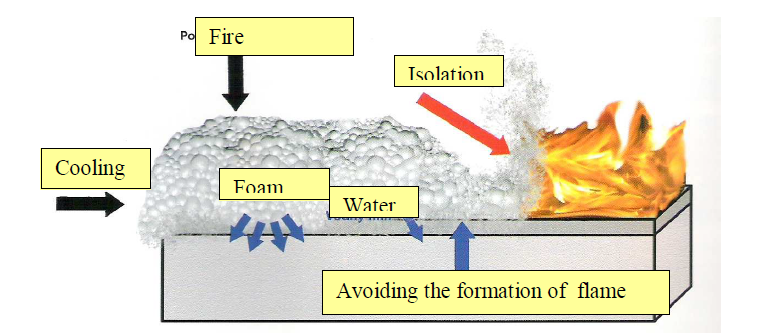
\includegraphics[width=.8\textwidth]{extinguishing_mechanism_scheme.png}
    \caption{Scheme of the extinguishing mechanism by using firefighting foam \cite{turekova2011environmental}}
    \label{ch2:figure:scheme}
\end{figure}

\section{Evolution of \acrshort{afff} for effective extinguishment of Class B fires}
Water has long been a universal agent for suppression of fires, however, it is not exceptional in all instances \cite{hinnant2020characterizing}. For instance, water is regularly incapable of suppressing combustible fluids and can be perilous. Protein-based foams which presented a drastic improvement over water for combating liquid fuel fires were developed and used initially. These protein-based foams are thick and form a heavy, heat-resistant covering over a burning liquid surface \cite{scheffey1995evaluating}. These properties made protein-based foams to be constrained as they were not able to spread rapidly over the fuel surface. This was a concern for a long time, as protein-based foams were not much effective in low viscosity fuels such as kerosene that is commonly used in aviation industry. The ineffectiveness was due to the inability of protein-based foams to spread rapidly.

Synthetic based foams were developed and introduced in the mid-1960s to optimize protein-based foams \cite{aamodt2020review} . These firefighting foams included \acrshort{afff} and \acrshort{ar-afff}. They generally provide better flow and spreading over the burning fuel surface, for faster knockdown of flames. \acrshort{afff} concentrates are made from blending fluoro-and hydrocarbon-surfactant, modest quantities of salts and foam stabilizers are regularly included \cite{wang2019research}. The \acrshort{afff} concentrate is then mixed with a specific level of water to form a foam solution. The proportioning rate is usually, 1\%, 3\% and 6\% of foam concentrate to water. Furthermore, an additional feature of 'aqueous film' is formed on the surface of a flammable liquid by the foam solution as it drains from the foam blanket \cite{hinnant2020characterizing}. This film is very fluid and floats on the surface of most hydrocarbon fuels, hence providing \acrshort{afff} with tremendous speed during extinguishing conditions. This made \acrshort{afff} to be further developed and predominant to most firefighting foams. Moreover, the introduction of \acrshort{afff} represented a significant increase in firefighting performance in terms of more rapid control and extinguishment of fuel fires, especial in industries that are involved with low viscosity fuels. The vital chemical composition of \acrshort{afff} are depicted in Table A.1 on appendices.

It is essential to comprehend that Class B fires are exothermic reaction that relies significantly upon four (4) elements: fuel, air/oxygen, heat, and chemical chain reaction \cite{beneventi2001role}. Removing one element will effectively halt the fire.  However, all firefighting foams do not interfere with the chemical reaction when extinguishing fuel fires, yet four (4) suppression mechanisms are required for knockdown and burn-back resistance:

\begin{itemize}
    \item The foam blankets the fuel surface smothering the fire. 
    \item The foam blanket separates the flames/ignition source from the fuel surface. 
    \item The foam cools the fuel and any adjacent metal surfaces. 
    \item The foam blanket suppresses the release of combustible fumes that can mix with air \cite{beneventi2001role}. 
\end{itemize}

All firefighting foams were developed for suppression of specific combustible fuels. It is vital to identify which fuel group is involved when flammable fire conditions occur. This is to ensure timeous and effective extinguishment during fire conditions. As a consequent, firefighting foam may be ineffective when used on unsuitable fuel, hence may yield unexpected or unfavorable outcomes. There are two different basic flammable or combustible fuel groups:

\begin{itemize}
    \item Standard hydrocarbon fuels such as gasoline, diesel, kerosene, jet fuel etc. these fuels do not blend with water or are not miscible in water, they usually float on top of water and, for the most part, they do not intermix.
    \item Polar solvent or Alcohol type fuels are fuels that mix readily with water or are miscible in water \cite{beneventi2001role}.
\end{itemize}

To date, \acrshort{afff} has been widely used in aviation fire protection for suppression of hydrocarbon fuels (a part of Class B fires). This synthetic based foam has a low viscosity and spreads quickly across the surface of most hydrocarbon fuels. Initially, \acrshort{afff} was developed for aviation industries due to the fuel (kerosene) they are involved with and have proven to be effective in several cases. However, they can also be relatively utilized for extinguishing Class A fires. During firefighting a water film forms underneath the foam, which cools the liquid fuel, halting the formation of combustible fumes \cite{scheffey1995evaluating}. Consequently, this gives a sensational fire knockdown, which is a critical aspect in crash rescue firefighting.

\section{Foam generating process}
Foam, in general, is created by a mechanical action (dispensing equipment), hence the generation of firefighting foam is a mechanical process that comprises numerous prior steps. There are various methods of generating firefighting foam, each method relies on the class of fire involve and foam solution used. To date, there are three (3) methods of generating firefighting foam from a foam solution namely: aspirated nozzle, \acrfull{caf}, and chemical reaction method \cite{laundess2012suppression}. The distinctions in these methods yield unique characteristics of foam produced with noticeable contrasts being the size and uniformity of the bubbles produced using each method \cite{laundess2012suppression}. Such differences may lead to significant variation of foam performance during fire conditions. However, the aspirated nozzle is a traditional and widely used method of generating firefighting foam, particularly in aviation fire protection.

Aviation fire protection have adopted the technique of aspirated nozzle when generating foam. This technique is more useful for aviation fire protection due to the type of environment and aviation standards that were developed and led by the \acrfull{nfpa}. Technically and according to the research, the aspirated nozzle is suitable for low expansion foams such as \acrshort{afff} and \acrshort{ar-afff} \cite{xi2017experimental}.  Aviation fire protection utilizes \acrshort{afff} for fire suppression due to the class of fuel (Jet A-1) they are involved with. Subsequently, the aspirated nozzle technique has been compatible with \acrshort{afff}. However, during the periodic tests in aviation, the functionality of this technique is tested and according to the reports, there are still concerns when using it \cite{laundess2012suppression}. Moreover, the gaps exist in the optimization of this foam generation.

Comprehending of various foam generation methods is essential in the present research work in order to evaluate and deduce if any other method can yield any benefits. Most Research have been focusing on the aspirated nozzle and \acrshort{caf} generation methods aiming to optimize or implement new methods. Optimization of these methods require complex mathematical analysis as there are numerous parameters involved. Besides, the complexity further relies on the variation of chemicals involved in the chemical reaction technique.

In the present study, the aspirated nozzle technique is evaluated against \acrshort{caf} and chemical reaction methods in order to minimize or eliminate the optimization challenges of this foam generation method in aviation fire protection. The experimental work conducted by Laundess et al \cite{laundess2012suppression} shows that foam generated by \acrshort{caf} technique displays uniformly small size bubbles, aspirated nozzle produces a greater spread of bubble sizes while chemical (nitrogen) reaction displays most uniform size distribution of bubbles as shown in Figure \ref{ch2:figure:characteristics}. In addition, the \acrshort{caf} method has the advantage of being environmentally friendly.  With the aspirated nozzle technique having environmental concerns, a new technique or optimization has emerged as an alternative in aviation fire protection.

\begin{figure}[H]
    \centering
    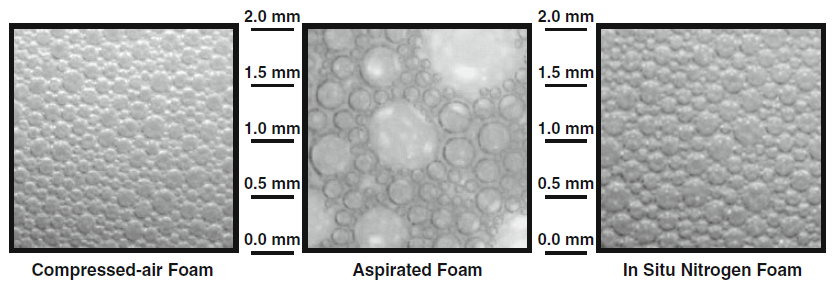
\includegraphics[width=.95\textwidth]{bubble_characteristics.png}
    \caption{Bubble characteristics for different generation methods \cite{laundess2012suppression}.}
    \label{ch2:figure:characteristics}
\end{figure}

\subsection{Aspirated nozzle}
The technique has been extensively used and is the traditional way of generating firefighting foam. In this method, foam is generated by extracting air into a jet of foam solution inside a nozzle \cite{xi2017experimental}. Most firefighting foam nozzles are specially designed in a convergent geometry. In this way, parameters such as pressure, velocity, and flow rate are carefully controlled as shown in Figure \ref{ch2:figure:nozzle}, foam solution at high pressure and low velocity enters the orifice at 1 and exit as finished foam at low pressure and high velocity at 5, at a constant flow rate. During stages 2, 3, and 4 air is drawn by a jet and blended with foam solution resulting in a strong mixing and agitation \cite{csb2016phenomenological}.

\begin{figure}[H]
    \centering
    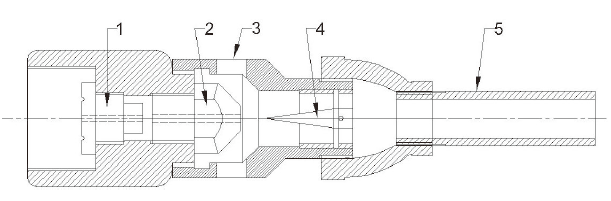
\includegraphics[width=\textwidth]{foam_generating_nozzle.png}
    \caption{Nozzle for generating foam \cite{csb2016phenomenological}.}
    \label{ch2:figure:nozzle}
\end{figure}

The governing equation for critical parameters during the foam generation is usually the Bernoulli's equation, which is given as:

\begin{equation}
    P_1+\frac{1}{2}\rho{v_1}^2 + \rho gh_1 = P_5+\frac{1}{2}\rho{v_5}^2 + \rho gh_5
\end{equation}

As seen in Figure \ref{ch2:figure:nozzle}, in case where the potential energy at the elevation 1 ($\rho gh_1$) equals the potential energy at elevation 2 ($\rho gh_5$), then the equation can be simplified and written as:

\begin{equation}
    P_1+\frac{1}{2}\rho{v_1}^2 = P_5+\frac{1}{2}\rho{v_5}^2
\end{equation}

\begin{doublespace}
    Where, \\
    $p_1\ is\ the\ pressure\ at\ elevation\ 1\ in\ Pa$ \\
    $v_1\ is\ the\ velocity\ at\ elevation\ 1\ in\ m/s$ \\
    $h_1\ is\ the\ height\ at\ elavation\ 1\ in\ m$ \\
    $P_5\ is\ the\ pressure\ at\ elavation\ 2\ in\ Pa$ \\
    $v_5\ is\ the velocity\ at\ elavation\ 2\ in\ m/s$ \\
    $h_5\ is\ the\ height\ at\ elevation\ 2\ in\ m$ \\
    $g\ is\ the\ acceleration\ due\ to\ gravity\ in\ m/s^2$ \\
    $\rho\ is\ the\ density\ of\ fuid\ in\ kg/m^3$ \\
\end{doublespace}

Since convergent nozzles are used to increase the outlet velocity ($v_5$  in figure \ref{ch2:figure:nozzle}) due to the conservation of mass, while critically maintaining the inlet flowrate during firefighting. Therefore, the following assumptions can be made:

\begin{gather*}
    A_1 > A_5 \\
    V_1 > V_5 \\
    P_1 > P_5
\end{gather*}

When the areas of the inlet and outlet are known and the flow rate that must be achieved is also known, then velocities can be calculated using the following equation:

\begin{equation}
    Q = VA
\end{equation}


\begin{doublespace}
    Where, \\
    $Q\ is\ the\ flowrate\ in m^3/s$ \\
    $V\ is\ the\ velocity\ of\ foam\ solution in m/s$ \\
    $A\ is\ the\ area\ of\ the\ nozzle\ at\ a\ particular\ point\ in\ m^2$ \\
\end{doublespace}

Over the years, researchers have been focusing on the source of these problems in order to comprehend the mathematical difficulties involved. However, engineers have been working on mathematical solution techniques in order to optimize convergent foam nozzles in aviation fire protection. Aspirated nozzle problems are noticeable during periodic trainings and uncertainty in the origination of the problem is mostly the challenge for many researchers.

\subsection{\Acrfull{caf}}
The \acrshort{caf} method is commonly used for generating any kind of firefighting foam and was developed initially by the \Acrfull{nrcc} in the late 1990s \cite{rie2016class}. The technique has offered several benefits in fire protection since the prohibition of halogen-based agents due to some environmental impacts.  

\acrshort{caf} technique is similar to the aspirated nozzle method as it also consists of a divergent nozzle for discharging foam. The distinction is that, in the \acrshort{caf} system, air is pressurized using an air compressor then fed or injected in an aqueous foam solution, as the foam expands its then discharges and guided through a nozzle.

\subsection{Chemical reaction}
This is a modern technique that was discovered by \cite{laundess2012suppression} to eliminate foam generation problems. The method has not yet been recognized in fire protection standards but certainly has several benefits. With other generation methods extensively used to produce much heavier carbon dioxide bubbles, it was of great practical significance to evaluate other methods that will produce lighter uniform bubbles. Consequently, nitrogen gas bubbles were the empirical and realistic alternative. In this way, the chemical reaction of foam solution and nitrogen creates numerous, uniformly sized bubbles of nitrogen gas within the foam.

The method has been reviewed by many researchers.  The only concern is the need to optimize foam formulations to prevent surfactants from being affected by the nitrogen generation and by the presence of salts formed during chemical reaction \cite{laundess2012suppression}.  For this reason, aviation fire protection will need to examine this as an alternative of possibly eliminating the aspirated nozzle method.

\section{Foaming ability and Mechanical stability}
Modern firefighting foams are primarily of the mechanical type. This means that before being utilized, they should be proportioned (mixed with water) and aerated (blended with air). Four elements are necessary to produce a quality and stable foam blanket and they include: foam concentrate, water, air, and aeration (mechanical agitation) \cite{oguike2013study}.

In recent years, mechanical stability has been a concern for most firefighting foams. Many researchers have approached this challenge with the aim of optimization. Foaming ability is a key process in advancing the mechanical stability of firefighting foams. Foam is a collection of air bubbles produced from a foaming solution \cite{oguike2013study}. The rate of this transformation is essential for evaluating the mechanical stability of the foam. Stability properties, as well as the effectiveness of firefighting foams, are determined by their physical and chemical properties, as described by Turekova and Balog \cite{turekova2011environmental}. These properties may include: the number of foaming, viscosity, foam frost resistance, the content of the sediment, foam stability, half-life of foam, pH, foaming solution of spreading factor \cite{turekova2011environmental}.

Synthetic based foams are low viscosity foams, consequently, they spread easily on the surface of the flammable liquid. This enables the formation of a dense and stable foam layer that acts as a physical boundary against the heat and mass transfer, thus exhibiting excellent cooling and covering effects in hydrocarbon fires \cite{xu2020fire}. The mechanical stability of \acrshort{afff} depends upon the structure of surface films from the so called-foaming agents. During firefighting conditions, the foams are continuously disrupted by the influence of heat of ignition, the internal force of foam, and the hot surface of burning liquid \cite{turekova2011environmental}. Foaming ability is thus a fundamental procedure as it directly affects the quality, hence the performance of the foam. The important parameters affecting a foam's ability to extinguish hydrocarbon fuel fire was addressed by Joseph et al \cite{scheffey1995evaluating} as shown in Figure \ref{ch2:figure:parameters}, with a theoretical modeling to further evaluate the challenges and limitation of the current methods used. 

\begin{figure}[H]
    \centering
    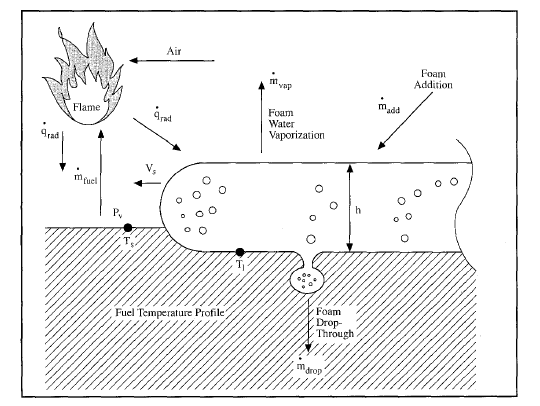
\includegraphics[width=\textwidth]{important_parameters.png}
    \caption{Important parameters affecting a foam's ability to exthinguishh hydrocarbon fuel fire \cite{scheffey1995evaluating}.}
    \label{ch2:figure:parameters}
\end{figure}

Oguike \cite{oguike2013study} conducted experimental tests intending to assess the foaming ability of various foams. The analysis comprised of eight (8) empty bottles, different volume of water was added and a constant foam concentrate was also added. The bottles were shaken vigorously at a steady time in each case and foam height was recorded. The foams were left to stand for some time and heights were measured again. Foams were left to stand for further days and height was measured again. Finally, foams formed were left to stand until collapse, and time was recorded for each foam solution. This experiment set a benchmark for most researchers, as most of the other foaming ability experiments have been based on it.

The current challenge is to develop small-scale test methods that measure these parameters in such a way that they can be used to predict large-scale foam performance. Persson \cite{persson1992fire} described optimization techniques and results to investigate foam mass loss by evaporation as a function of radiant heat from a fire. The finding was that foam viscosity and spreading is an area requiring further investigation. 

\subsection{\acrshort{afff} blanket stability/drainage time}
Drainage time is often used to analyze the stability of various foams, however, it does not provide a reliable indication of the firefighting capability of foams. Drainage time is a measurement of the rate at which foam solution drains out of finished foam and hence provides an indication of the stability of the foam blanket \cite{aamodt2020review}. High expansion foams usually maintain the stability and heat resistance due to their long drainage time and hence slow loss of water from the finished foam. 

Since \acrshort{afff} is a low expansion foam, there are difficulties in maintaining the stability and heat resistance from the finished foam. This is due to short drainage time which indicates that finished foam losses its water content rapidly and renders it vulnerable to high-temperature flames and hot surfaces. A basic principle of measuring low expansion foam expansion ratios is shown in Figure \ref{ch2:figure:tests}. In recent years, most researchers concluded that the drainage times of finished foams do not solely depend on foam concentrate but also the type of foam generation \cite{martin2012fire}. In most cases, drainage time for low expansion foams such as \acrshort{afff} is often expressed as 25\% drainage time, while for medium and high it's usually 50\% drainage time. This is the time taken for 25\% or 50\% of the original foam solution content (by volume) to drain from the finished foam, as shown in Figure \ref{ch2:figure:tests}.

\begin{figure}[H]

\centering
\begin{subfigure}{.45\textwidth}
    \centering
    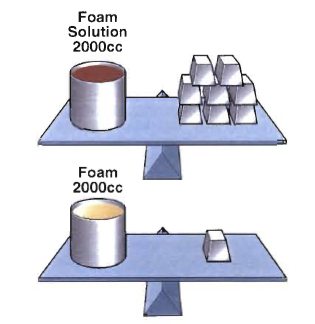
\includegraphics[width=\textwidth]{low_expansion_test.png}
    \caption{}
\end{subfigure}
\begin{subfigure}{.45\textwidth}
    \centering
    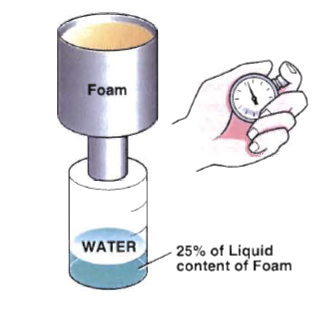
\includegraphics[width=\textwidth]{drainage_test.png}
    \caption{}
\end{subfigure}

\caption{a) Low expansion test and b) drainage test \cite{aamodt2020review}.}
\label{ch2:figure:tests}
\end{figure}

Researchers have been working on optimizing the foaming ability, hence the stability of foams, particularly for low expansion foams.  An experimental work to analyze and compare the drainage time and bubble size distribution of various firefighting foams was described by Mark et al \cite{laundess2012suppression}. Table \ref{ch2:table:times} shows the results of \cite{laundess2012suppression} comparing the 25\% of drainage times at an expansion ratio of 7:1 for two different foam concentrates. \\

\begin{table}[H]
\caption{Comparison of 25\% drainage times at 7:1 expansion \cite{laundess2012suppression}.}   

\centering
\begin{tabularx}{\textwidth}{>{\hsize=1.1\hsize}X >{\hsize=1.1\hsize}X >{\hsize=.89\hsize}X >{\hsize=.89\hsize}X >{\hsize=.89\hsize}X >{\hsize=1.1\hsize}X}
    \hline
    \multicolumn{6}{c}{Mean Drainage time (s)} \\
    \hline
    Foam \allowbreak concentrate & Generation system & Mean & Max & Min & Standard \allowbreak Deviation \\ 
    Tolomet 6\% & ISNF & 342 & 450 & 264 & 93 \\
    & \acrshort{caf} & 488 & 533 & 430 & 53 \\
    & Aspirated & 197 & N/A & N/A & N/A \\
    FC-600 3\% & ISNF & 539 & 725 & 450 & 126 \\
    & \acrshort{caf} & 1060 & 1281 & 844 & 288 \\
    & Aspirated & 485 & N/A & N/A & N/A \\
    \hline
\end{tabularx}

\label{ch2:table:times}
\end{table}

The results indicate that drainage rates for the various foam types were quite different, which may be explained by differences in the bubble size distributions as discussed below in Figure \ref{ch2:figure:distributions}. To explain the differences in foam drainage rates between the three foam types, they studied the bubble size distributions for each foam type.

\begin{figure}[H]
    \centering
    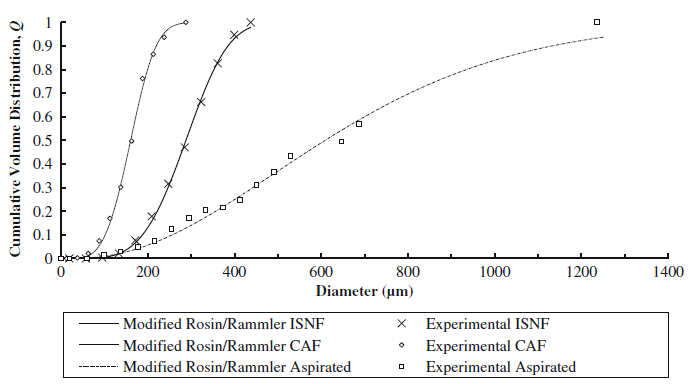
\includegraphics[width=\textwidth]{bubble_size_distributions.png}
    \caption{Cumulative bubble size distributions for various foam generation methods \cite{laundess2012suppression}.}
    \label{ch2:figure:distributions}
\end{figure}

As shown in Figure \ref{ch2:figure:distributions}, the drainage time is profoundly dependent upon the foam generation type. Also, the aspirated foam generation method produced larger bubbles in terms of size. These bubbles contributed to shorter drainage times as seen in Table \ref{ch2:table:times}, hence the reduction of foam quality and stability. This correlation technique used was benchmarked by \cite{oguike2013study} and most researchers have concluded the same as \cite{laundess2012suppression}. Mukunda and Dixit \cite{csb2016phenomenological} constructed a model of foam drainage based on momentum flux balance and conducted experiments with an apparatus with foam drainage through a fuel layer. Their results showed a linear relationship of 25\% drainage time with the height consistent with the theoretical expectations. A recommendation made by \cite{laundess2012suppression} indicates that there is a need for further research to develop a new surfactant formulations immune to the oxidation reaction that generates nitrogen bubbles. This foam generation method will simultaneously increase the drainage rates and stability of low expansion foams due to nitrogen bubbles.

\section{Critical application rates}
In the most recent decade, most researchers have been interested in the application rates of various firefighting foams. A number of studies on effective application rates have increased significantly and most of these studies have been based on protein and synthetic based foams. The underlying motivation for considering diverse critical application rates was to identify the compatibility of foams on various class of fires. With the original motivation behind the development of synthetic based foams being economic issues, the application rates were, thus critical.

Most of the research on firefighting foams are based on optimization aiming to provide the necessary effectiveness and efficiency in performance. The basis for the current minimum application rates was originally developed in 1972 by Geyer \cite{geyer1972evaluation} in tests of protein and \acrshort{afff} solutions. These were "modelling" tests with \acrfull{jp-4} pool fires that measured 21 m, 30 m, and 43 m in diameter. They also included large-scale verification tests with a B-47 aircraft and simulated shielded fires, conducted with \acrshort{jp-4} pool fires 34 m and 43 in diameter with all tests conducted using air-aspirating foam generation method. The outcomes by \cite{geyer1972evaluation} showed that PF and \acrshort{afff} have an application rate with a ratio of 1.49:1 respectively and is shown in Figure \ref{ch2:figure:pool}. This difference in application rate recognizes the inherent advantage of using \acrshort{afff} to extinguish hydrocarbon pool fires and reflects the fact that \acrshort{afff} has been demonstrated to extinguish pool fires more rapidly than PF at equivalent application rates. For equivalent extinguishment times, lower rates of \acrshort{afff} than PF are required \cite{scheffey1995evaluating}.

\begin{figure}[H]
    \centering
    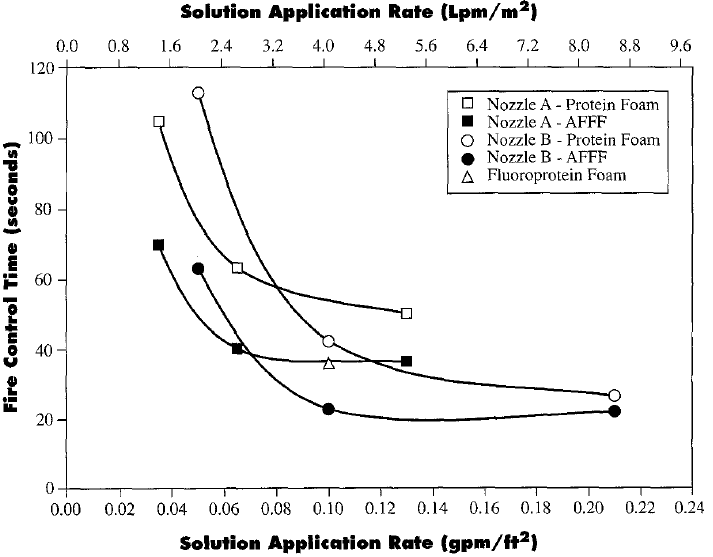
\includegraphics[width=\textwidth,height=11cm]{fire_control_time_pool_fires.png}
    \caption{Fire control time as a function of solution application rate using protein foam and \acrshort{afff} on \acrshort{jp-4} pool fires \cite{geyer1972evaluation}.}
    \label{ch2:figure:pool}
\end{figure}

Numerous experimental tests have been conducted by many researchers with purpose of validating these application rates. Geyer et al \cite{geyer1979comparative} further conducted tests on critical application rates for validation. The experimental tests conducted were focused on fire control time as a function of solution application rate for PF, AFF, and FPF for Jet A fuel fires and the results are shown in Figure \ref{ch2:figure:fuel}. These were aiming in employing more foam generation methods and different fire type to make necessary analyses of outcomes and compare with \cite{geyer1972evaluation}. Based on Figure \ref{ch2:figure:pool} and \ref{ch2:figure:fuel}, the application rate is greatly dependent on the type of foam generation and also the type of foam concentrates utilised. There have been numerous challenges regarding the critical applications of firefighting foams. The proliferation of performance guidelines and specifications for firefighting foams has created divergent opinions especially on aviation industry fire protection standards \cite{scheffey1995evaluating}.

\begin{figure}[H]
    \centering
    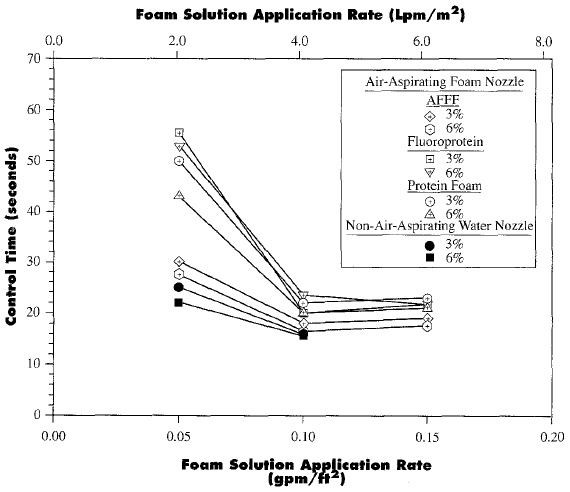
\includegraphics[width=\textwidth,height=11cm]{fire_control_time_fuel_fires.png}
    \caption{Fire control time as a function of solution application rate for \acrshort{afff}, fluoroprotein and protein foams for Jet A fuel fires \cite{geyer1972evaluation}.}
    \label{ch2:figure:fuel}
\end{figure}

\section{Effect of degradability}
Aircraft accidents are currently not a threatening issue in South Africa. This is due to a drastic decrease in air-crash over the past years. Nevertheless, fire protection in South African aviation has always been compliant. Due to this drastic decrease in air-crash, firefighting resources including firefighting foam last a long time without actually being realistically tested. Firefighting foams naturally degrade over time due to several factors such as liquid drainage driven by gravity and coarsening. Firefighting foam degradation is defined by Hinnant et al \cite{hinnant2017influence} as a reduction in foam layer thickness regardless of any changes in foam density or 'quality'.

In the present research work, it is essential to comprehend the impact of different storage facilities on foam degradation. In this way, advancing the storage facility focusing on degradation will be uncomplicated. Aviation periodic training is the only platform of testing foam performance parameters, hence foam degradation. As a result, it may not indicate the precise causes of degradation as this is not an actual situation. Foam's effectiveness can be severely deteriorated by foam degradation. Thus, foam degradation can be influenced by many factors including the hot fuel, fire, and foam formulation that contains surfactants and additives needed to generate the foam \cite{hinnant2017influence}. Although these factors are known, some of them such as fuel and fire cannot easily be controlled.    

During the firefighting process, foam is continuously interacting with fuel and flame. The interaction may immensely destroy the thick layer of the foam \cite{osei2015foam}. In this way, the ability of foam will be reduced, thus its performance may be compromised. However, foam degradation may suddenly increase dramatically during this process.  The causes for this are not well understood due to the lack of research on foam degradation. Furthermore, the individual effect of fire and fuel on degradation are inseparable due to the presence of fire \cite{hinnant2017influence}. 

Previous research on foam degradation has mostly focused on the natural aging process of foam \cite{do2011numerical} and the effect of the interaction of hydrocarbon liquids with foam \cite{osei2015foam}.  The natural aging of foam can be mainly influenced by the storage tank utilized, which is essential in this research work as the optimization of the storage facility based on degradation will be benchmarked by these previous Research. Hinnant et \cite{hinnant2017influence} studied the influence of fuel on foam degradation for fluorinated and fluorine-free foams. The study outcome showed that the fuel temperature is by far the major factor contributing to foam degradation followed by the effects of surfactant formulation, type of fuel, and bubble diameter or expansion ratio. Figure \ref{ch2:figure:degradation} shows the percentage change in \acrshort{afff} thickness versus time at room temperature, 35, 50, 75, and 90℃.

\begin{figure}[H]
    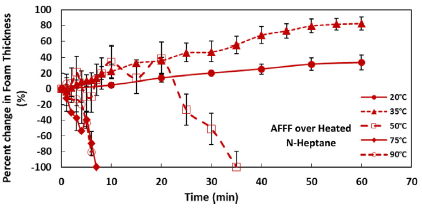
\includegraphics[width=.65\textwidth]{foam_degradation.png}
    \caption{\acrshort{afff} foam degradation versus time over n-heptane fuel at different temperatures \cite{hinnant2017influence}.}
    \label{ch2:figure:degradation}
\end{figure}

Parameters such as bubble diameter or expansion ratio are much dependent on the foam generation method, which is discussed in section 2.4. Larger bubbles cause a rapid drainage rate than smaller bubbles, and according to \cite{hinnant2017influence}, the increased drainage rate can cause the foam to degrade rapidly. In this way, the storage facility may indirectly affect foam degradation. This is due to the sediments or sludge, which may accumulate in the storage facility during the aging process. Consequently, sediments may affect foam characteristics, particularly bubble distribution during the foam generation process, this is shown by employing a flow process in Figure \ref{ch2:figure:effect}. The optimization of a storage facility in reducing the accumulation of sediments will prove to extensively reduce foam degradation.

\begin{figure}[H]

\centering
\begin{adjustbox}{center}
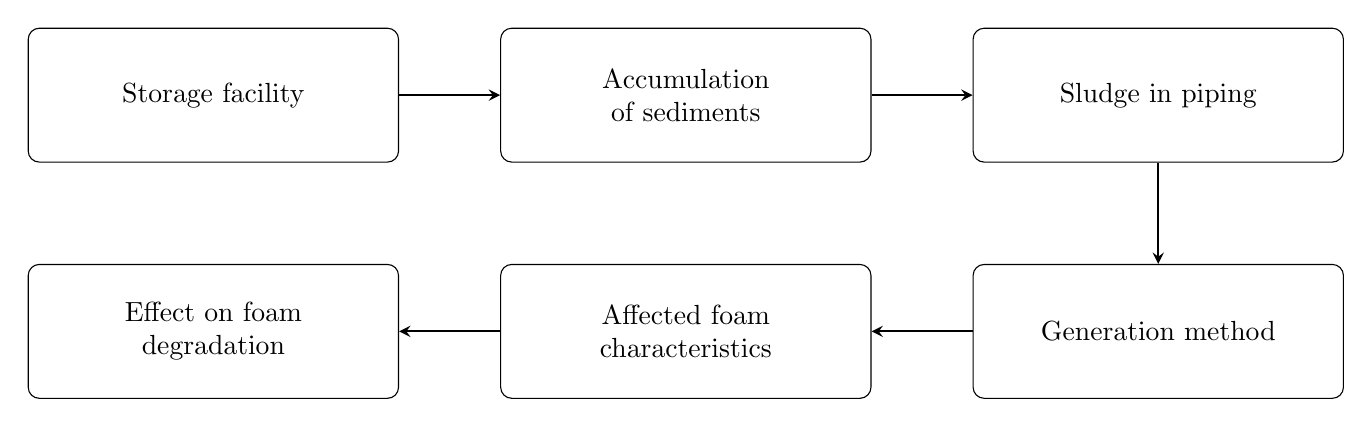
\begin{tikzpicture}[node distance=6cm]
    \tikzstyle{block} = [rectangle, rounded corners, draw, text centered, text width=4cm, inner sep=1em, minimum height=1.7cm]
    \tikzstyle{arrow} = [thick,->,>=stealth]

    \node (storage) [block] {Storage facility};
    \node (accumulation) [block, right of=storage] {Accumulation of sediments};
    \node (sludge) [block, right of=accumulation] {Sludge in piping};
    \node (generation) [block, below of=sludge, yshift=3cm] {Generation method};
    \node (affect) [block, left of=generation]{Affected foam characteristics};
    \node (effect) [block, left of=affect] {Effect on foam degradation};

    \draw [arrow] (storage) -- (accumulation);
    \draw [arrow] (accumulation) -- (sludge);
    \draw [arrow] (sludge) -- (generation);
    \draw [arrow] (generation) -- (affect);
    \draw [arrow] (affect) -- (effect);
\end{tikzpicture}
\end{adjustbox}

\caption{Effect of \acrshort{afff} degradation.}
\label{ch2:figure:effect}
\end{figure}

There have been fewer studies on the effect of surfactant formulation on degradation, further research should be conducted to detect the effect of this parameter on foam degradation. Furthermore, other parameters that may affect foam degradation should be extensively investigated in the future as foam degradation may regularly affect the performance of the foam.

\section{Environmental issues}
Modern firefighting foams can be considered as sensational in terms of physical characteristics, but, in recent years, the new Registration Evaluation Authorization and Restriction of Chemicals (REACH) legislation have drawn attention to their ecotoxicological properties \cite{turekova2011environmental}. While \acrshort{afff} is the most widely used firefighting foam in aviation fire protection, it still has some disadvantages, of which one of those is the environmental impact \cite{zhao2016improving}. Due to growing concerns regarding the impact that firefighting foams have on the environment, steps need to be taken to rectify this situation. To date, few papers have looked at the environmental impact of \acrshort{afff}. This lack of research on environmentally friendly surfactants must be addressed with more experimental studies to reduce the contamination of the environment, especially in aviation industry.

Although \acrshort{afff} has numerous advantages over other firefighting foams, their environmental issues have been a huge setback. Initially, \acrshort{afff} contained substances such as perfluoroalkyl and poly-fluoroalkyl (PFAS). Previous research shows that PFAS had significantly caused the contamination of soil, groundwater, and surface water including water stream animals as a result of \acrshort{afff} being released during aviation periodic training \cite{milley2018estimating}. As shown in Figure \ref{ch2:figure:use}, this poses acts of negligence and is hazardous to the environment as foam detoxifies naturally in soil.

\begin{figure}[H]
    \centering
    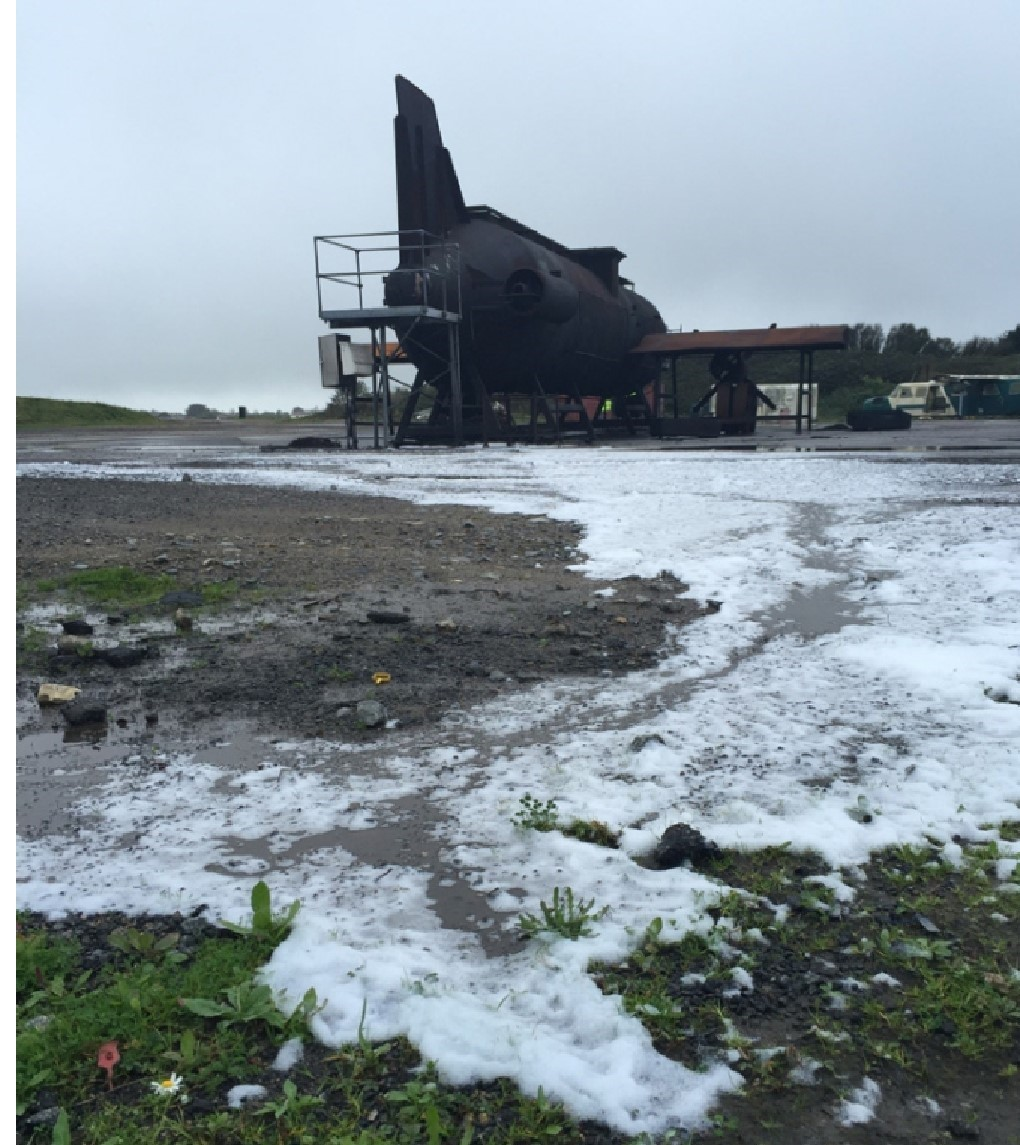
\includegraphics[width=\textwidth,height=9cm]{use_during_aviation_training.jpg}
    \caption{Used \acrshort{afff} during aviation periodic training.}
    \label{ch2:figure:use}
\end{figure}

Initially, PFAS's have not been previously known or recognized to be harmful in the environment. This was due to the complexity of \acrshort{afff} mixtures utilized and previous significant gaps in thorough comprehending of PFAS, including their toxicity, bioaccumulation, occurrence, transport, and transformation mechanisms \cite{milley2018estimating}. However, PFAS's impact in the environment was then recognized in the late 1990s and several jurisdictions offered guidance with a limited range or amount of PFAS's that can impact the environment \cite{hinnant2017influence}.

Elimination of PFAS in \acrshort{afff} was a challenge for every manufacturer and aviation industries as these chemical substances were key during fire suppression. \acrshort{afff} was able to suppress fire rapidly due to the presence of PFAS's. With environmental regulations enforcing the elimination of PFAS, manufacturers had no other alternative but to cooperate in the elimination of PFAS's. Consequently, PFAS's were phased out in 2002 by all the manufacturers due to the environmental impact \cite{persson2003foamspex}.  Fluorinated surfactants replaced PFAS's instantly intending to reduce the environmental impact and still be compatible with \acrshort{afff}. 

According to the research, fluorinated surfactants were also found to have an impact on the environment \cite{martin2012fire}. As a result, samples that were analyzed in 2010 indicate that \acrshort{afff} manufacturers have commenced to gradually reduce or even eliminate fluorinated surfactants in their formulations \cite{milley2018estimating}. Moreover, this process of eliminating present surfactants is critical as the transition should be carefully analyzed, in order to prevent the possible negative influence, it might pose in the performance parameters of firefighting foam. To date, fluorinated surfactants are present in \acrshort{afff} and are continuously bio-persistent in the environment and pose health hazards to humans.

The main objective of the present research work is to improve the compatibility of the materials that are utilised to construct the storage facility. Therefore, the environmental issues of \acrshort{afff} are of significance in the present study, since the optimised storage materials should not negatively influence the composition of \acrshort{afff}, as this might then cause environmental issues during firefighting. 

In recent years, researchers have been investigating the effective ways of mitigating the environmental issues. While the progress of this optimization has been held back by the difficulties stated above. The \acrshort{nfpa} committee, which is responsible for \acrshort{nfpa} 11, \emph{low expansion foams}, has made significant effort in tasking a group to address the environmental concerns around low expansion foams \cite{scheffey1995evaluating}. The outcome of the task group has been recently published with a full guidance to end user\cite{scheffey1995evaluating}. Alternatively, researchers have managed to implement new surfactants which are environmentally friendly. However, commercial firefighting foams without fluorinated surfactants developed to date have not been able to extinguish the fire as rapid as \acrshort{afff} \cite{hinnant2017influence}. In the future, researchers will need to conduct an extensive investigation in order to implement the environmentally friendly surfactants that will be compatible with \acrshort{afff}.  

\section{Conclusions}
This chapter reviewed the relevant literature to gain a better and in-depth understanding of the various firefighting foams. The focus was diverted to \acrshort{afff}, where the evolution of this type of foam was studied. Various foam generation processes were discussed, and their impacts on the poor performance of \acrshort{afff}. Based on the previous studies, the aspirated nozzle is suitable for generating \acrshort{afff}. The equations involved during this process were analyzed, with some recommendations to optimize this process being detailed. The importance of the foaming ability and mechanical stability were addressed, and the findings of previous studies were discussed. It was then found that the stability directly affects the quality, hence the performance of the foam.

The next chapter evaluates the various engineering materials commonly used to construct the storage facility for \acrshort{afff} concentrate. It further investigates and recommends possible ways of enhancing the properties of these materials based on the current knowledge.
\chapter{Evaluation of construction materials}
\section{Introduction}
This chapter details an in-depth understanding of the engineering materials commonly used to construct the storage facility for \acrshort{afff} concentrate. The scope of this chapter includes a brief overview of these materials to thoroughly understand how they are classified. It further details the properties of interest for each material and why they opted as storage facilities.

Fundamental literature concerning the evolution of these materials is detailed in this chapter. The corrosion phenomenon is investigated in each material to understand its effect on the performance parameters of \acrshort{afff}. Furthermore, an understanding of the metallic bonding and cross-linking of these materials is vital. This is briefly discussed in this chapter. To improve the properties of these materials, the microstructure morphology must be better understood. This also aided when analyzing the microstructure of each material in chapter \ref{ch6:anchor:chapter}. In this way, is possible to optimize these materials once the metallic bonding, cross-linking, useful properties, and microstructure are well comprehended. Subsequently, the heat treatment processes are evaluated to make an effort of optimizing these engineering materials.

\section{A brief overview of construction materials}
As the economy becomes increasingly global, the importance of materials increases. Storage facilities/tanks can be constructed using a variety of materials. The selection of the material can be a challenging systematic process that is commonly dependent on cost, reliability, availability, ease of fabrication, material properties, and environmental impacts (\cite{hench2005biomaterials}).  The main goal to be achieved in this process is to minimize the cost while meeting the product performance, efficiently. However, for storage facilities, it may largely depend on the type of product to be stored. The product to be stored may vary in the state or phase of matter, which is critical to evaluate before any process commences. To date, there are five (5) different states of matter that are known: solids, liquids, gases, plasma, and Bose-Einsten condensate (\cite{ceruti2002states}).

For the present research work, the evaluation of the construction material will focus on the liquid state, since \acrshort{afff} concentrate is in liquid form. In this way, the material that will be used to construct the storage facility can be significantly evaluated. The classification of engineering materials is shown in the form of a flow chart in Figure \ref{ch3:figure:materials}.

\begin{figure}[H]
    \centering
    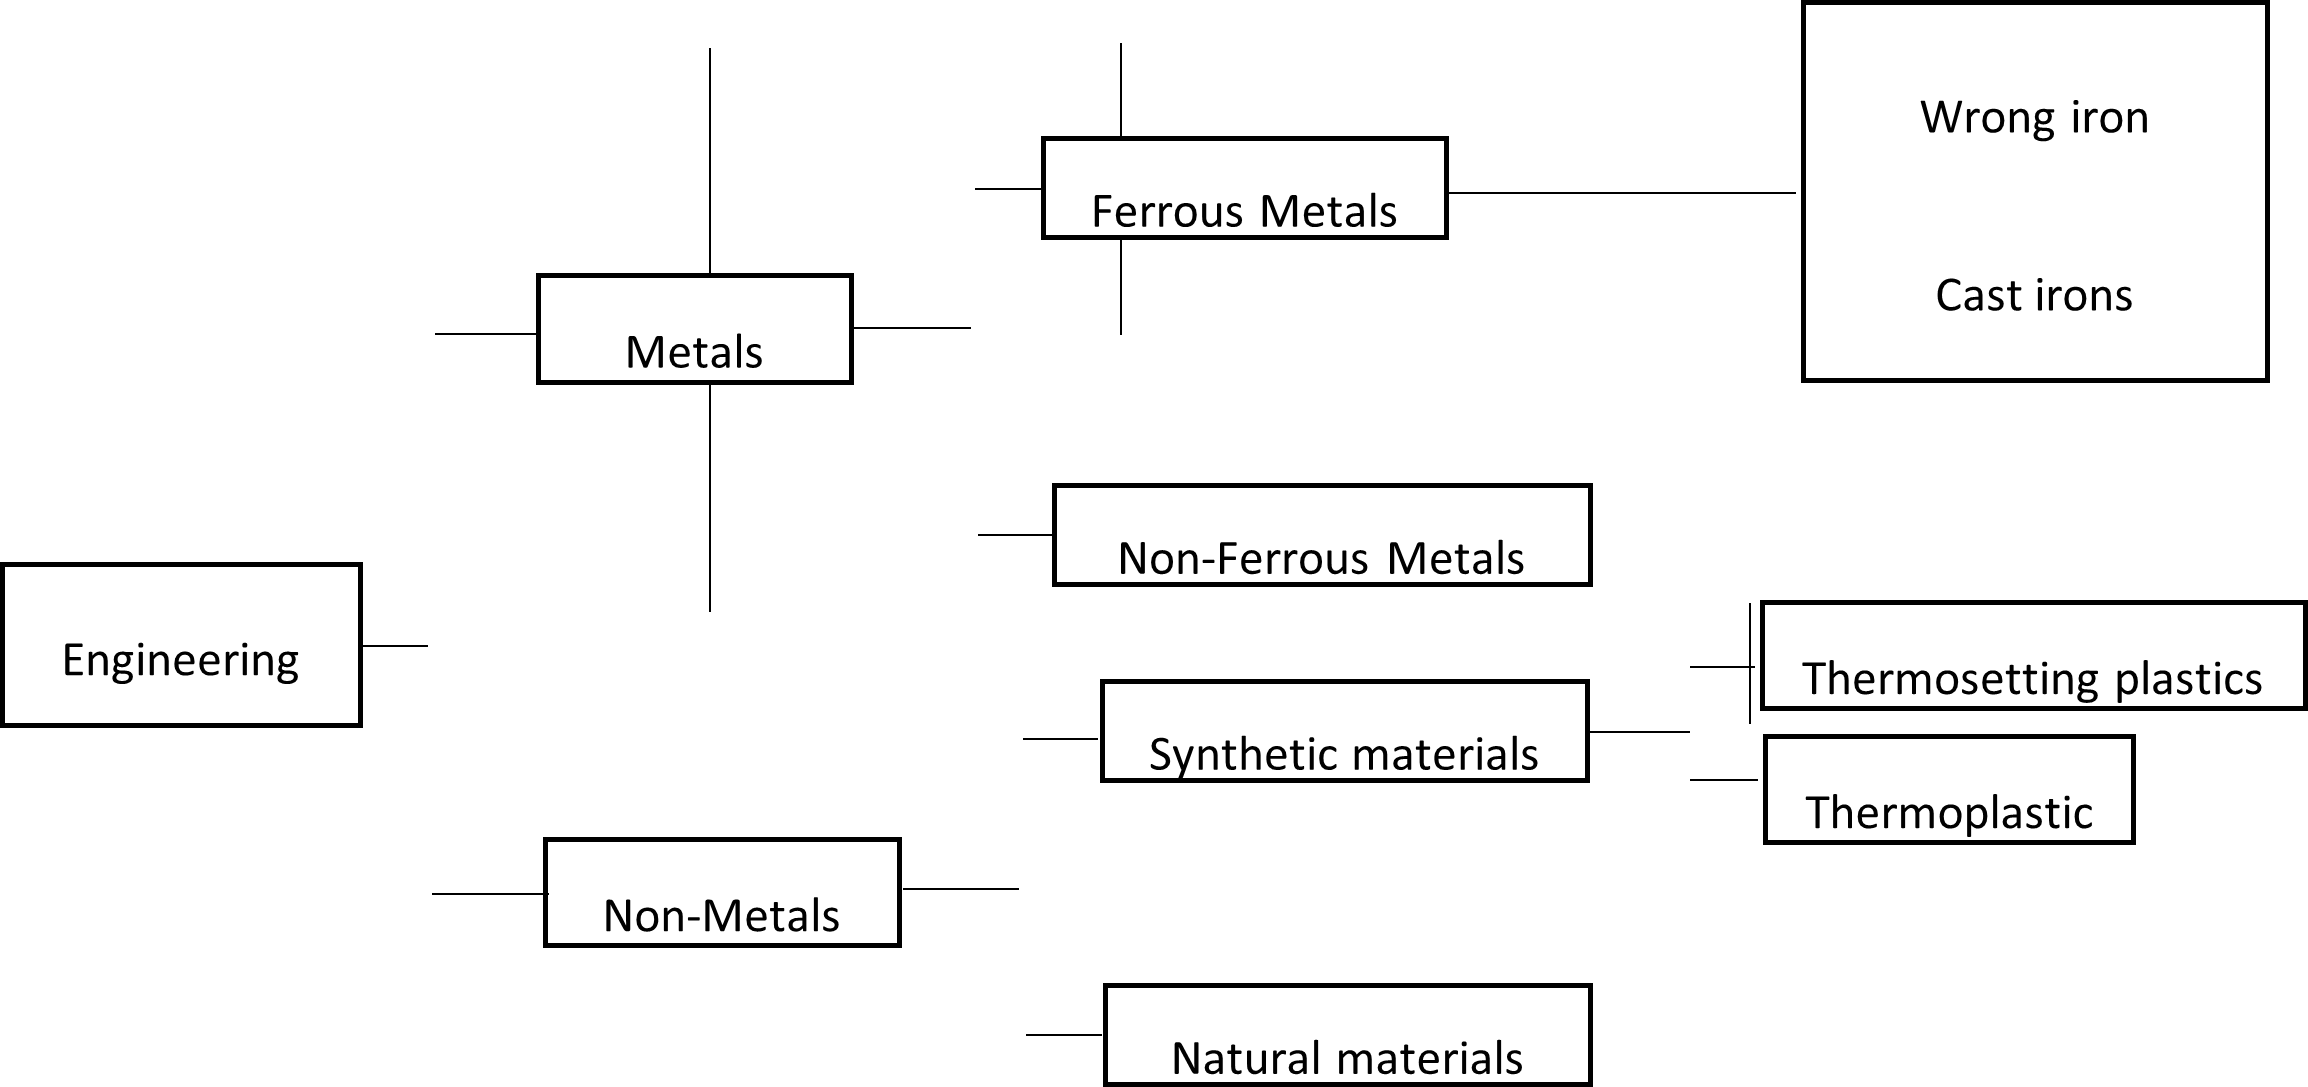
\includegraphics[width=\textwidth]{materials_classification.png}
    \caption{Engineering materials classification (\cite{timings2008fabrication})}
    \label{ch3:figure:materials}
\end{figure}

Material selection is not a new era, it is a large and traditional branch of engineering materials. Moreover, it requires technical expertise. Material properties can be decisive when evaluating the storage facility material of construction. Material property is defined as an intensive property of a material that is not influenced by the amount of the material (\cite{mcarthur2004engineering}). Typically, these are the properties we can measure or test. These properties can continuously interfere with the product stored in the storage tank; hence it is crucial to thoroughly comprehend them. There are several properties of materials, but in the present study, the following broad properties: physical and mechanical will be carefully investigated, with an effort of improving these properties, thus ensuring the compatibility of the storage facility material of construction with \acrshort{afff} concentrate.

It is vital to decide whether you are investigating the properties of the material or an object, as this could cause a contradiction. For example, you should decide whether you are identifying the properties of the storage facility or the properties of the material it is constructed of. Properties such as the shape and mass of the object (storage facility) may vary, even when they are constructed of the same material. It is for the same reason that it is assumed that the construction structure of the storage facility can have an impact on the performance parameters of \acrshort{afff}.  In other instances, material properties can be improved by processes such as mixing, heating, and cooling (heat treatment). This may be useful as the improved properties may yield better performance. For this reason, it is of great significance to evaluate the surrounding environmental factors that may change the initial material properties, thus affecting the \acrshort{afff} concentrate in that process.

Traditionally, storage facilities were constructed using metallic materials. However, in the last decade, researchers have developed specialized non-metallic materials in the form of composite materials to enhance materials that are utilized to construct storage facilities. These exceptional materials have diverse and combined properties that produce even better performance for storage facilities. Nevertheless, these advanced materials have some limitations and challenges that are notable during the specialized manufacturing technique.

This section gives an overview of the current materials that are used to construct the \acrshort{afff} concentrate storage facilities. First, the material characteristics and properties of metallic materials are discussed and carefully evaluated. Since non-metallic materials are gradually emerging, then their properties and limitations are also discussed. Finally, the four common materials used in the present study are specified, and various concerns regarding these materials are analyzed to identify and close the possible gaps that currently exist.

\subsection{Metallic materials}
Metallic materials are a significant part of engineering materials and have been extensively studied and used for a variety of purposes.  In material sciences, metallic materials are inorganic substances that usually contain a combination of metallic elements, which may also contain small amounts of non-metallic elements (\cite{ali2020empirical}). The typical combination of metallic elements could be metals such as gold, iron, titanium, aluminium, etc. The small amount of non-metallic could be elements such as carbon, nitrogen, oxygen, etc (\cite{hench2005biomaterials}). In physical sciences, there are 118 elements on the periodic Table, and 86 of these belong to the metallic group (\cite{ali2020empirical}). All these 86 metals have diverse characteristics, and a limited number of these can be significantly used for engineering and other purposes.

In the last century, scientists have been working tirelessly to significantly understand these types of materials to develop efficient techniques that will aid in the optimization of metallic materials. With that being said, over the last 70 years, scientists have developed new techniques for producing various materials with enhanced properties to those of natural materials (\cite{ali2020empirical}). To date, numerous metallic materials such as gold and copper mostly rely on these new techniques to yield effective performance. Consequently, metallic materials are rarely utilized as authentic elements, thus they are usually blended with other elements to form an alloy (\cite{hench2005biomaterials}). Many storage facilities are constructed using alloy metals due to their distinctive characteristic properties.

The metallic materials are broadly classified as ‘ferrous and non-ferrous’ (\cite{ali2020empirical}). Ferrous metals are those that contain iron (Fe) elements within them, while non-ferrous metals do not contain any iron element. In the present study, only ferrous metals will be discussed. Ferrous metals are vital in the present study, as mild and stainless steel materials will be experimentally evaluated when used as an \acrshort{afff} storage facility.  Mild and stainless steels are regarded as ferrous metals due to the presence of iron in their structure. Usually, ferrous metals suffer from the ‘corrosion phenomenon’ due to the presence of iron. Ferrous materials constitute more than 50\% of the metallic materials section (\cite{ali2020empirical}). Furthermore, these materials (ferrous) are useful in numerous applications as they meet the various service requirements of our modern and complex society.

While scientists have managed to develop efficient techniques for producing metals, it was of great importance to understand the relationship between structural elements of the materials and their properties. In the textbook ‘engineering materials science’ by \cite{mcarthur2004engineering}, the microstructure is defined as the arrangement of crystals (or grains) of the different phases. Hence, these are observed when a polished section of a piece of the material is viewed at high magnification through a microscope (\cite{molabe2018determining}). The chapter on metallic materials has been studied extensively. As a consequence, it has been experimentally proven over the past decades that the properties of metallic materials are interrelated with the microstructure of the material itself. This is evidence that the properties can be enhanced by altering the relative proportions of the micro-constituents (or phases). Phases are identified by their unique crystal structures, composition, and properties (\cite{mcarthur2004engineering}).

Liquid storage facilities are critical in ensuring that the properties of the stored products are well maintained. Metallic materials have offered numerous and diverse benefits when utilized as liquid storage facilities. However, in other instances horrible incidences that result in storage facility catastrophic failure occur. This proves that although metallic materials are beneficial, there are still gaps that exist, probably in the metal production optimization, enhancing of natural properties, and relevant materials selection. There are relatively three factors that may influence the choice of metals and alloys when used as an \acrshort{afff} storage facility:

\begin{itemize}
    \item Mechanical, physical, chemical, and thermal properties.
    \item Degradation of the material.
    \item Compatibility with the product to be stored, which is \acrshort{afff} for the present study.
\end{itemize}

Understanding relevant material selection will aid in easing the enhancement of the properties of metallic materials. This will be more useful in metallic materials that are widely utilized to construct the storage facility for storing \acrshort{afff} concentrate. 

\subsection{Metalic bonding}
In general, the term ‘bonding’ can be described as the action of joining two or more things firmly, especially employing adhesive, heat, or chemical bonds (\cite{soler2000metallic}). In materials and science, there are three types of bonding: covalent, ionic, and metallic bonding. For the present study, the focus will be on evaluating and comprehending metallic bonding.

In the early 1900s, Paul Drüde discovered the metallic bonding theory by modelling metals as a mixture of atomic cores (positive nuclei + inner shell of electrons) and valence electrons (\cite{sinex2017general}). Metallic bonding can be described as the type of chemical bond formed between positively charged atoms in which the free electrons are shared among a lattice of cations (\cite{lepetit2017topological}). In contrast, covalent and ionic bonds form between two distinct atoms. Metallic bonding in the major type of chemical bonding that forms between metal atoms. Figure \ref{ch3:figure:bonding} shows how a metallic bond occurs.

\begin{figure}[H]
    \centering
    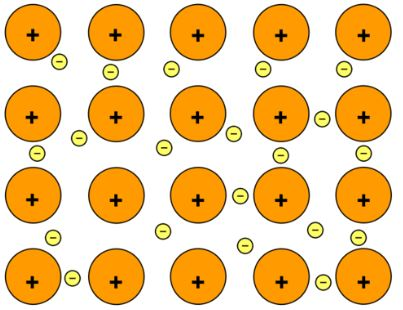
\includegraphics[width=.5\textwidth]{metalic_bonding.jpg}
    \caption{Metalic bonding: Positive atomic nuclei (orange circles) surrounded by delocalized electrons (yellow cirlces) (\cite{soler2000metallic}).}
    \label{ch3:figure:bonding}
\end{figure}


Metallic bonds are commonly noticed in natural metals, alloy metals, and some metalloids. For instance, graphene (an allotrope of carbon) usually reveals two-dimensional metallic bonding (\cite{lepetit2017topological}). It should be noted that metals, including natural ones, are not limited to metallic bonding. Thus, they have the capability of forming other types of chemical bonds within their atoms.

All atoms contain a small nucleus of neutrons and protons these are surrounded by orbiting electrons (\cite{hench2005biomaterials}). Distinct atomic models can be significantly used to describe different properties of the overall material. As previously stated, one beneficial model of a metal is a repeating structure of metallic ions, which are surrounded by a ‘sea’ of electrons, see Figure \ref{ch3:figure:bonding}. It is the ‘free electrons’ that critically determine the thermal and physical properties of the metallic material (\cite{hench2005biomaterials}). Alternatively, several mechanical properties of metallic materials can be better understood by considering atoms to behave like ‘hard spheres’ (\cite{hench2005biomaterials}). This is vital in the present study as this will be used as a benchmark in improving the properties of alloy metals that are commonly utilized as \acrshort{afff} storage facilities.

When atoms are behaving like hard spheres, they are relatively bonded together by an attractive force (\cite{lepetit2017topological}). However, this type of bonding is very weak, which is the reason why metals have a crystalline structure where atoms are significantly arranged in a dense, regular, and repeating manner. The atoms of various metals are significantly arranged in various crystal structures (\cite{hench2005biomaterials}). Atoms in metallic materials can be relatively arranged in four (4) different ways these include face-centred cubic (\acrshort{fcc}), \acrfull{hcp}, body-centred cubic (\acrshort{bcc}) and tetragonal. A typical example may include a pure metal such as aluminium (Al) in which atoms are relatively arranged in \acrshort{fcc} at room temperature (\cite{hench2005biomaterials}), as shown in Figure \ref{ch3:figure:aluminium}.
 
\begin{figure}[H]
    \centering
    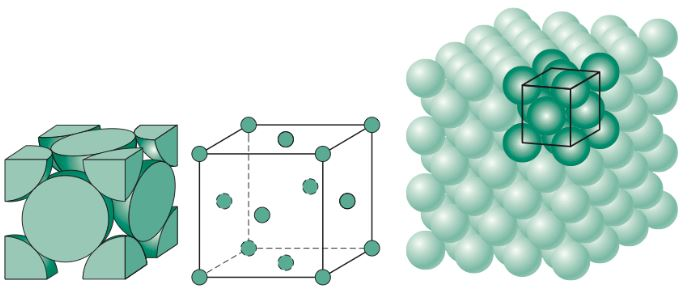
\includegraphics[width=\textwidth]{aluminium_crystal_structure.jpg}
    \caption{Crystal structure of aluminium metal (Al) at room temperature (\cite{hench2005biomaterials}).}
    \label{ch3:figure:aluminium}
\end{figure}

The mentioned crystal structures are determined at room temperature.  However, the transition in the crystal structure is much more possible in several metals. This transition varies with the temperature to which the metal is exposed (\cite{callister2018materials}). For example, metals such as pure iron may reveal two different crystal structures. At room temperature it reveals \acrshort{bcc}, but when the temperature is constantly increased towards a melting point (912-1394℃), its crystal structure changes to \acrshort{fcc}. Further increasing the temperature to about 1538 ℃ will result in reverting the crystal structure to \acrshort{bcc} (\cite{ali2020empirical, molabe2018determining}). For alloy metals, the transition in the crystal structure can be achieved by adding an element with a different crystal structure. The transition in alloy metals will be evaluated in detail in Section \ref{ch3:anchor:section:morphology}. Table \ref{ch3:table:structure} shows the atom arrangement in a crystal structure of some commonly used pure metals.

\begin{table}[H]
\caption{Crystal structure for popular metals, at room temperature (\cite{hench2005biomaterials}).}

\begin{tabularx}{.8\textwidth}{ XX }
    \hline
    Metal & Crystal structure \\
    \hline
    Aluminum & FCC \\
    Chromium & BCC \\
    Copper & FCC \\
    Gold & FCC \\
    Iron & BCC \\
    Silver & FCC \\
    Nickel & FCC \\
    \hline
\end{tabularx}

\label{ch3:table:structure}
\end{table}

Several physical and mechanical properties of materials are determined by the metallic bonds and the arrangement of the atoms in the crystal structure. For example, when metallic material is heated to a melting point, the atoms have to gain sufficient energy to break free from the crystal structure (\cite{hench2005biomaterials}). This is evidence that the properties of materials can be altered by altering the arrangement of atoms in a crystal structure. Moreover, the crystal structure significantly determines the ability of atoms to slip over one another during the deformation of metals (\cite{callister2018materials}). This is especially true in ductile metals due to their ability to deform without easily breaking. These types of materials are commonly used to construct liquid storage facilities due to their crystal structure that yields exceptional properties.

\section{Mild steel material}
\label{ch3:anchor:section:material}
Mild steel is a ferrous metal that contains a relatively low content of carbon, which usually ranges from 0.05\% to 0.25\% by weight (\cite{callister2018materials}). Thus, it is also known as 'low-carbon steel.  Low-carbon steels consist primarily of ferrite rather than perlite (\cite{li2018effect}). Metals containing carbon content from 0.30 to 2.0\% are typically referred to as higher carbon steel (\cite{timings2008fabrication}). The addition of carbon content increases the strength of the steel. Consequently, steel materials having a carbon content higher than 2\% are often regarded as ‘cast-iron' (\cite{callister2018materials}).  Mild steel is a popular metallic material that has been extensively used for many applications, including industrial storage facilities.

Although mild steel contains carbon, iron, and other elements in its composition, it nonetheless cannot be regarded as alloy steel. This is due to the extremely low amount of carbon and other alloying elements it contains; thus, these elements are insufficient to produce alloy steel. The relatively low amount of carbon and other alloying elements in the composition of mild steel results in diverse properties when compared to higher carbon and alloy steels (\cite{timings2008fabrication}). The high content of iron and ferrite in the composition of mild steel means that it is magnetic (\cite{li2018effect}).

Low-carbon steels are generally useful in liquid storage facility construction, due to their compatible properties. In particular, mild steel is one of the most commonly used tank construction materials. It is popularly known for its ductility and can be made from readily available natural materials. The low cost of this metal makes it beneficial to numerous industries in terms of economic.

The low-carbon steel setback to date has been corrosion, which causes more serious deterioration problems in storage facilities(\cite{erami2019carboxamide}). Various coatings have been developed over the past decade, aiming to mitigate this problem. The other major concern regarding low-carbon steels is that it is nearly impossible to alter some of the mechanical properties through heat treatment (\cite{callister2018materials}). Moreover, low-carbon content means that mild steel has very few alloying elements to prevent dislocation in the crystal structure, resulting in less tensile strength than high-carbon and alloy steels (\cite{callister2018materials}).

This section provides and evaluates mild steel as a material and also as an object (storage facility). The scope of this section includes the evaluation of the current properties and their impacts on the \acrshort{afff} storage facility. Similarly, the understanding of the microstructure of low-carbon steels to develop useful strategies to improve the properties and compatibility of this metallic material is essential for the present study. The machinability of low-carbon steels is evaluated. Furthermore, the corrosion concerns are discussed, and common methods to prevent this are briefly discussed. Finally, the heat treatment processes that are commonly used to enhance the properties are also closely assessed. This will aid in understanding the gaps in the optimization of the properties.

\subsection{Useful properties} 
As previously stated, the material property is a comprehensive property that is not dependent upon the amount or size of the material (\cite{kabir2020critical}). These are the quantitative parameters that are measurable/tested and observed when a load is applied. As a consequence, these properties are significantly determined by the composition and crystal structure of the material. Thus, it is vital to understand the arrangement of atoms in the crystal structure. Furthermore, before any material is selected for a certain application, the properties should be immensely understood to ensure compatibility with the application utilized.

Mild steel has a variety of properties that makes it beneficial for several applications and these are detailed in Figure \ref{appendix:carbon_steel_properties} in the appendices. These properties can be broadly grouped into mechanical and physical properties (\cite{kabir2020critical}). These two properties are vital determinants for which metal is considered to be compatible with a given application. In almost every instance, mechanical properties are interdependent, meaning high performance in one category may be achieved with lowering performance in other categories (\cite{kabir2020critical}). For example, the low content of carbon in mild steel means that this metallic material is more ductile when compared to alloy steel.

For low-carbon steels, ductility indicates that they can be formed into the desired shape at any temperature without major difficulties (\cite{dong2005deformation}). Figure \ref{ch3:figure:carbon} shows how the carbon content of plain carbon steel affects the properties of the steel. Referring to Figure \ref{ch3:figure:carbon} it can be observed that altering carbon content in plain carbon steels has an impact on the properties. Consequently, when the carbon content has increased, the ductility of the steel materials is relatively decreased. Moreover, the strength and hardness are remarkably increased, which results in the transition from ductile to brittle (\cite{abou2001mechanical}). For liquid (\acrshort{afff}) storage facilities, ductility is one of the significant properties. This property means that the storage facility can be rolled or joined using various mechanical fabrication methods mentioned in Section 4.3.1, without having major concerns.
 
\begin{figure}[H]
    \centering
    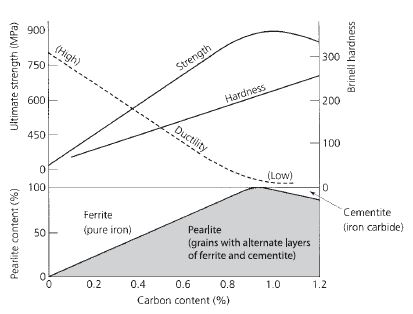
\includegraphics[width=.65\textwidth]{effect_of_carbon_content.jpg}
    \caption{Effect of carbon content on the properties of plain carbon steel (\cite{timings2008fabrication}).}
    \label{ch3:figure:carbon}
\end{figure}

Another critical parameter for storage facilities constructed of mild steel is thermal conductivity, which falls under physical properties. In the textbook, ‘heat transfer: a practical approach’ by \cite{cengel1998heat} thermal conductivity is defined as a measure of the quantity of heat that flows through a material. In the present study, the storage facility does not necessarily need to be constructed with materials that have a high thermal conductivity. However, achieving this is somehow difficult, due to the diverse properties a material can have.

Mild steel has a thermal conductivity of 64.86 $\nicefrac{W}{m.K}$ at most (\cite{cengel1998heat}). This is quite less when compared to other steels but can be considered high for applications that do not require heat transfer. At extremely high temperatures, heat may be transferred to the product inside the storage tank and may influence the viscosity of the product. For the present study, heat transfer is not a concern, due to the environment (atmospheric), the storage facility is located on. However, when looking at this from another perspective, it can cause problems along the time. When the storage facility is continuously exposed to high-temperature environments, heat can be gradually transferred until it causes some notable problems to \acrshort{afff} solution. To reduce heat transfer, insulating materials are usually utilized, but they however do not eliminate the problem completely. As a consequence, it is vital to understand the environmental factors that may associate with the properties of the material on the location of the storage facility.

There are normally three means of transferring heat namely conduction, convention, and radiation. Conduction involves heat transfer through solid materials, convention is associated with heat transfer between a solid surface and a gas or liquid that is in motion, while radiation is the energy emitted by the matter in the form of electromagnetic waves (\cite{cengel1998heat}). In the case of \acrshort{afff} storage facilities, heat transfer by conduction is of great interest, as this is the possible scenario in this circumstance.   

For the worst situation, the total heat energy that can be transferred to the storage facility, hence \acrshort{afff} concentrate as a result of the surround atmosphere (radiation) can be calculated using the energy balance equation as follows:

\begin{equation}
    Q_c = m \times C_p \times \Delta T
\end{equation}

\begin{doublespace}
\noindent Where, \\
$Q_c\ is\ the\ amount\ of\ net\ heat\ transfer\ to\ the\ system\ in\ J$ \\
$m\ is\ the\ mass\ of\ a\ material\ in\ kg$ \\
$C_p\ is\ the\ specific\ heat\ capacity\ in\ \nicefrac{kJ}{kg.^\circ C}$ \\
$\Delta T\ is\ the\ temperature\ difference\ of\ surfaces\ in\ ^\circ C$ \\
\end{doublespace}

When the total heat energy that is being transferred to the storage tank holding \acrshort{afff} is known, it is now vital to estimate the rate at which this heat energy is being transferred. This is critical in predicting whether the composition of \acrshort{afff} concentrate is being affected by the heat that is transferred to the storage facility by conduction. The equation for calculation of conduction heat transfer rate is known as Fourier’s Law of Heat Conduction and is given by:

\begin{equation}
    Q_c = -k \times A \times \frac{\Delta T}{\Delta r}
\end{equation}


\begin{doublespace}
\noindent Where, \\
$Q_c\ is\ the\ conductive\ heat\ transfer\ rate\ in\ W$ \\
$k\ is\ the\ thermal\ conductivity\ of\ thematerial\ in\ \nicefrac{W}{m.^\circ C}$ \\
$A\ is\ the\ cross-sectional\ area\ in\ m^2$ \\
$\Delta T\ is\ the\ temperature\ diifference\ of\ surfaces\ in\ ^\circ C$ \\
$\Delta r\ is\ the\ distance\ separating\ the\ surfaces\ in\ m$ \\
\end{doublespace}
In heat transfer, positive heat conduction means that heat is flowing into the body in question, and negative heat conduction represents heat leaving the body. Heat transfer has been applied in various research fields mainly to increase the heat transfer rate, decrease heat transfer rate and keep the temperature in a certain range. For the present study, the focus is to ensure a decrease in the rate of heat transfer, so that it will not suddenly change the composition of \acrshort{afff}, thus influencing its firefighting performance.  

Another property of interest for the present study is the effect of corrosion on steel. Corrosion is the process of decay of a material (usually ferrous metals) caused by a chemical reaction with its environment (\cite{islam2018effects}). \acrshort{afff} concentrate is generally not a corrosive type of liquid. However, mild steel contains about 98\% iron in its composition, which is significantly high and makes it to be considered a corrosive ferrous metal.  The corrosion phenomenon is usually prevented in several ways, and these will be discussed in detail in Section \ref{ch3:anchor:section:effects}.


\section{Stainless steel material} 
Stainless steels are ferrous metallic materials that contain a minimum of 10.5\% of chromium and about 8\% of nickel as the main alloying element (\cite{sourmail2005stainless}). All the alloying elements have a significant role in the stainless steel family. Chromium element forms a protective self-healing oxide film, which greatly improves the corrosion resistance of stainless steel (\cite{molabe2018determining}). Large amounts of nickel contribute to both heat and corrosion resistance (\cite{george2002introduction}). However, depending on the percentage of nickel added, it also contributes to high strength and excellent toughness. Other relevant elements are often added to enhance the properties of stainless steel. It is these alloying elements that make stainless steel to be generally more expensive than carbon steel.

\begin{figure}[H]
    \centering
    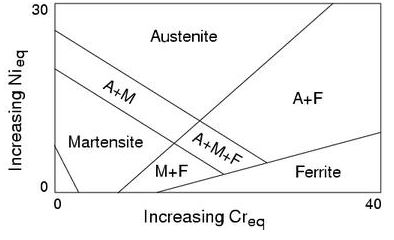
\includegraphics[width=.65\textwidth]{stainless_steel_phase.jpg}
    \caption{Stainless steel phase diagram as a function of chromium and nickel equivalents at room temperature (\cite{bhadeshia2017steels}).}
    \label{ch3:figure:steel_phase}
\end{figure}

The classification of stainless steel is based on the nature of its metallurgical structure (\cite{bhadeshia2017steels}). As previously stated in Section \ref{ch3:anchor:section:material}, the metallurgical structure is the arrangement of the atoms making up the grains of the steel. The microstructure is formed based on the chemical composition of the steel. With an appropriate combination of alloying elements that results in a unique microstructure, stainless steels can be fully austenitic, and a mixture of ferrite and austenite (duplex), fully ferritic or martensitic (\cite{bhadeshia2017steels}). These four possible microstructure phases are shown in Figure \ref{ch3:figure:steel_phase}. These categories of stainless steel are obtained under specific cooling conditions, and all are beneficial for various applications.
 
In the present research work, duplex stainless steel is of great significance. As can be seen in Figure \ref{ch3:figure:steel_phase}, the duplex contains a combination of austenite and ferrite, approximately 50\% of each. It is more beneficial and extensively used in liquid storage facilities, as it yields a combination of properties. This is due to a large amount of chromium and less nickel content presence, which results in corrosion resistance, high strength, and excellent toughness (\cite{gunn1997duplex}). The weighed composition of duplex stainless steel is detailed in Figure \ref{appendix:duplex_stainless_steel_properties} on appendices. The less content of nickel in duplex stainless steel implies that duplex is relatively inexpensive compared to other classes (\cite{sourmail2005stainless}). 

\begin{figure}[H]
    \centering
    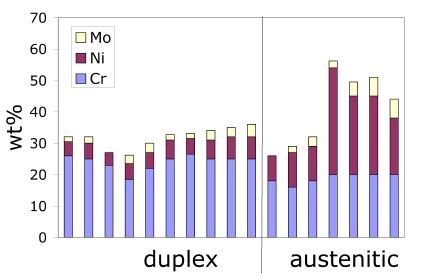
\includegraphics[width=.65\textwidth]{weight_percentages.jpg}
    \caption{Weight percentage of Cr, Ni, and Mo in duplex and austenitic steels (\cite{sourmail2005stainless}).}
    \label{ch3:figure:weight}
\end{figure}
The two-phase mixture also reduces the risk of intergranular attack; for the same reason, they are not prone to solidification cracking during welding (\cite{sourmail2005stainless}). Figure \ref{ch3:figure:weight} shows the comparison of the weight percentage of \acrfull{cr}, \acrfull{ni}, and \acrfull{mo} in duplex and austenitic stainless steel.
 
In general, stainless steel is an excellent metallic material that has several useful properties which are shown in Figure \ref{appendix:stainless_steel_properties} in the appendices. Consequently, this type of steel offers numerous benefits for various applications. Although stainless steel is popularly known for excellent corrosion resistance, reports in recent years have suggested otherwise (\cite{karayan2014weld}). Corrosion in stainless steel often occurs unexpectedly on the welded joints, which then affects the product that is stored, particularly in welded storage tank applications. Another concern for stainless steel is the difficulty in machinability (\cite{grzesik2008advanced}). Fabricating or manufacturing stainless steel is not an easy task, due to the elements it contains. All these concerns are greatly dependent on the microstructure of the material, and the possible optimization methods will be discussed in Sections \ref{ch3:anchor:section:morphology} and \ref{ch3:anchor:section:treatment} respectively.

\section{Effect of corrosion on steels}
\label{ch3:anchor:section:effects}
Corrosion is an integrative and critical subject of matter that has numerous half-truths and myths, which exist to date (\cite{mcarthur2004engineering}). These are continuously occurring due to ignorance when it comes to the science of corrosion.  Corrosion is a phenomenon that commonly affects ferrous metals due to the presence of iron. In corrosion science, corrosion is defined as the deterioration of a substance or its properties due to interactions between the substance and its environment (\cite{chigondo2016recent}).

In recent years, corrosion has become a vital matter in liquid storage facilities, especially in acidic liquids. Corrosivity is generally measured by either pH or the rate of steel corrosion (\cite{marzorati2018green}). When the aqueous concentrate has a Ph less than or equal to two, or more than or equal to 12.5, it is considered to be corrosive (\cite{marzorati2018green}). As a consequence, corrosion is generally not a concern in storage facilities containing \acrshort{afff} concentrate since it has an approximate Ph value of 7-8.5. However, the storage facility can nonetheless suffer from corrosion due to the surrounding environment. In the present research, a storage facility containing \acrshort{afff} concentrate is continuously exposed to the corrosive atmospheric environment (Durban, South Africa) due to the near sea. Figure \ref{ch3:figure:ph} shows the corrosive Ph level of an aqueous concentrate.
 
\begin{figure}[H]
    \centering
    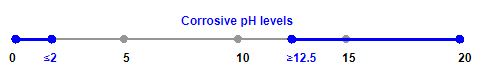
\includegraphics[width=.8\textwidth]{aqueous_solution_ph_scale.jpg}
    \caption{Ph scale for aqueous solution (\cite{marzorati2018green}).}
    \label{ch3:figure:ph}
\end{figure}

Although there is a lack or little knowledge of the corrosion phenomenon, some researchers have made significant efforts to understand it. The material is initially selected due to the desired properties. However, some recently published literature suggests that corrosion has a degrading effect on mechanical properties. \cite{li2018effect} conducted a study that concluded that corrosion can lead to a reduction of the thickness of the storage facilities, and thus in the reduction of yield strength, ultimate strength, and ductility on low carbon steels.  Marcus \cite{protopopoff2011surface} further stated that the reduction of these properties is due to hydrogen accumulation within the steel, which is known as \acrfull{he}. Besides, this accumulation of hydrogen results in a sudden reduction in the ductility of steel. Figure \ref{ch3:figure:degradation} shows the process of mechanical properties degradation due to corrosion.

In more detail, corrosion occurs when there is a combination of oxygen reduction and hydrogen evolution reactions, as shown in equations (\ref{ch3:equation:acid} – \ref{ch3:equation:neutralalkaline}) (\cite{li2018effect}).  Consequently, during these reactions, atomic hydrogen is released. It then eventually accumulates at the defects within the steel, forming molecular hydrogen. Finally, the molecular hydrogen results in the increase of inside pressure, and eventually micro-cracking initiations, which consequently degrades the mechanical properties of steel (\cite{whitman1924effect}).
 
\begin{figure}[H]
    \centering
    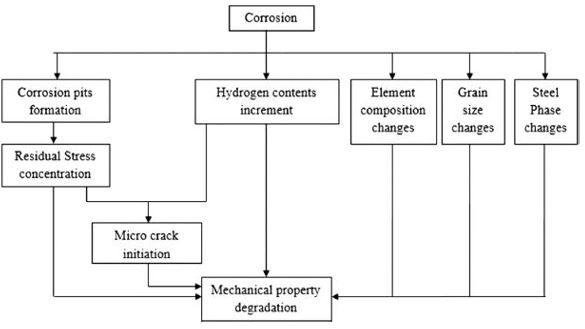
\includegraphics[width=\textwidth]{process_of_mechanical_properties.jpg}
    \caption{Process of mechanical properties degradation due to corrosion (\cite{protopopoff2011surface}).}
    \label{ch3:figure:degradation}
\end{figure}

Oxygen Reduction Reaction (ORR)

\begin{equation}
    \frac{1}{2}0_2 + 2H_3O^{+2e \rightarrow 3H_2OAcid}
    \label{ch3:equation:acid}
\end{equation}

\begin{equation}
    \frac{1}{2}O_2 + H_2O + 2e \rightarrow 2OH^{-Neutralalkaline}
\end{equation}

Hydrogen Evolution Reaction (HER)

\begin{equation}
    H_3O^{++e \rightarrow \frac{1}{2}H_2 + H_2OAcid}
\end{equation}

\begin{equation}
    H_2O + e \rightarrow \frac{1}{2}H_2 + OH^{-Neutral,alkaline}
    \label{ch3:equation:neutralalkaline}
\end{equation}

Based on Equations (\ref{ch3:equation:neutralalkaline} - 3.9), it is sensible to believe that corrosion changes the elemental composition of the steel. However, few papers focus on monitoring the changes in element composition during corrosion. Corrosion may also result in the degradation of mechanical properties by changing three microstructural features: (1) grain size, (2) phase composition, and (3) formation of corrosion pits (\cite{li2018effect}). Presumably, corrosion is interrelated with the microstructure of the material. For example, grain size reduction causes more hydrogen absorption within steel (\cite{li2018effect}). However, there are several limitations to existing Research. To begin with, the hydrogen embrittlement phenomenon has been mainly carried out for \acrfull{hsla} and stainless steel (\cite{li2018effect}). As a consequence, extensive research should be conducted to determine the degradation mechanism of mechanical properties due to corrosion, at both macro and micro levels.

Many researchers have been interested in the corrosion phenomenon, thus over the years, there have been several ways developed to prevent corrosion. Corrosion can occur in many ways, thus it is also significant to understand different types of corrosion and evaluate the corrosion of interest. Stainless and mild steel are the metallic materials of interest in the present study; thus, it is vital to understand the different ways in which corrosion occurs in these two metallic materials. In this way, it is possible to optimize the current methods that are utilized to prevent corrosion, focusing precisely on the corrosion of interest.

As previously stated, several half-truths and myths regarding corrosion exist. Stainless steel is popularly known for resisting corrosion due to the presence of a chromium element in its composition. However, these are myths and half-truths due to the incidences that have proven that stainless steel can suffer from corrosion. This is usually the case on welded products. In contrast, mild steel is well known for suffering from corrosion, this is due to the lack of corrosion-protecting alloying elements such as chromium (\cite{hackerman1987theory}). However, corrosion prevention is more practical than making an effort to eliminate it. A stainless steel storage facility that has suffered from corrosion on welded joints is shown in Figure \ref{ch3:figure:tank}.
 
\begin{figure}[H]
    \centering
    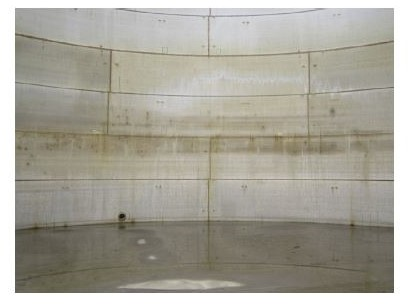
\includegraphics[width=.55\textwidth]{storage_tank.jpg}
    \caption{Storage tank that corroded on welded joints (\cite{karayan2014weld}).}
    \label{ch3:figure:tank}
\end{figure}

\subsection{Types of corrosion} 
The tendency of a metal to corrode depends upon the crystal structure of the metal, its composition as formed during alloying, and the temperature for deformation of a single metal surface developed during fabrication (\cite{sourmail2005stainless}). The environment plays a key role in the corrosion of the material; thus, it can vary with the environment to which the substance is exposed. Consequently, this makes it complex to comprehend the corrosion mechanism. Corrosion can be caused by diverse factors that include the reactivity of metal, the presence of impurities, the presence of air, moisture, gases like sulphur dioxide, and carbon (\cite{sourmail2005stainless}). Therefore, corrosion protection and prevention are significantly aimed at addressing these factors. There are various types of corrosion, and it is vital to understand which corrosion you are faced with. The different types of corrosion which depend upon the environment surrounding the material, type of material, or chemical reaction are briefly described in Table \ref{ch3:table:corrosions}.

\begin{table}[H]
\caption{Types of corrosion (\cite{chigondo2016recent}).}

\centering
\renewcommand{\arraystretch}{2}
\begin{tabularx}{\textwidth}{>{\hsize=0.65\hsize}X >{\hsize=1.35\hsize}X}
    \hline
    Type of corrosion & Description \\
    \hline
    Uniform corrosion & Deteriorates the whole surface of the metal and makes the surface thin. \\
    Galvanic corrosion & Occurs with an electrolyte with metal having different values of electrical potentials. \\
    Pitting corrosion & Occurs because of the random attacks on particular parts of the metal's surface to form pits. The pit acts as an anode, while the undamaged part of the metal is the cathode. \\
    Stress corrosion cracking & A complex form of corrosion which arises due to stress and  corrosive environment. \\
    Corrosion fatigue & A combination of cyclic stress and corrosion.  \\
    Intergranular corrosion & Corrosion occurs on or near the grain boundaries of a metal.  \\
    Crevice corrosion & Concentration cell corrosion due to the trapping of corrosive liquid  between the gaps of the metal. \\
    Filiform corrosion & Concentration cell corrosion on metallic surfaces coated with a thin  organic film. \\
    Erosion corrosion & Flow-assisted corrosion which is due to the movement of corrosive  liquids on metal surface. \\
    Fretting corrosion & A form of corrosion which shows the combined effect of corrosion and  fretting of metal. \\
    \hline
\end{tabularx}

\label{ch3:table:corrosions}
\end{table}

In the present study, the focus is on stress corrosion cracking/atmospheric corrosion. As can be observed in Table \ref{ch3:table:corrosions}, stress corrosion cracking is a complex form of corrosion which arises due to the stress and corrosive atmosphere. However, the cracking of the storage facility due to stresses is not a concern in the present study, thus the focus is particularly on the corrosive atmospheric environment.

\subsubsection{Atmospheric corrosion}
Atmospheric corrosion is a naturally occurring chemical deterioration of a material due to a reaction with the environment, especially with oxygen. The extent of deterioration of a ferrous metal depends on the chemical composition and grain structure of the material. For example, when iron is exposed to an industrial atmosphere for a long period, iron oxide, also known as rust, forms on the surface, as shown in Figure \ref{ch3:figure:corrosion} (\cite{mcarthur2004engineering}). The rust is very porous to oxygen and water in the atmosphere, and consequently, the corrosion process continues until the metal is entirely consumed (\cite{protopopoff2011surface}).  Atmospheric corrosion generally occurs in three various environments rural, industrial, and marine. For the present study, the industrial environment is the benchmark since the storage facility is located in an industrial environment. Figure \ref{ch3:figure:corroded} shows the storage facility, which was initially protected from corrosion yet ended up suffering from rural atmospheric corrosion.

\begin{figure}[H]
    \centering
    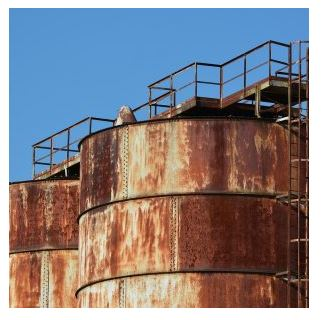
\includegraphics[scale=1.3]{corrosion_of_storage_facilities.jpg}
    \caption{Atmospheric corrosion of storage facilities in industrial environment (\cite{chigondo2016recent}).}
    \label{ch3:figure:corrosion}
\end{figure}
 
\begin{figure}[H]
    \centering
    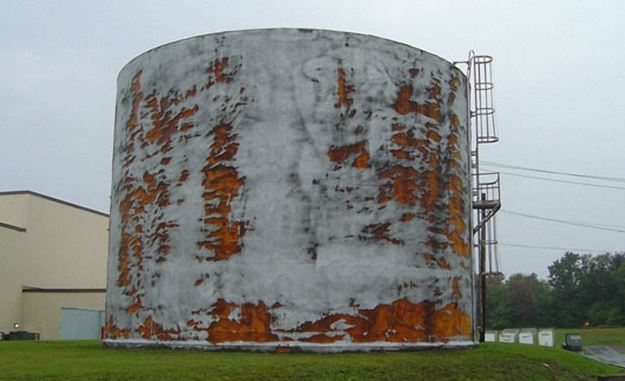
\includegraphics[width=\textwidth]{corroded_storage.jpg}
    \caption{Corroded storage facility (\cite{protopopoff2011surface}).}
    \label{ch3:figure:corroded}
\end{figure}

Atmospheric corrosion is one of the most common types of corrosion, which is affected by several environmental factors. It commonly affects infrastructure, transportation, energy, and other industries (\cite{pei2021understanding}). Over the decades, research has shown that contributing environmental factors affecting the outdoor atmospheric corrosion rate include temperature, \acrfull{rh}, atmospheric pollutants (commonly sulphur dioxide and chlorides), and wind (\cite{abou2001mechanical, islam2018effects}). It is difficult to individually analyse the impact of these factors due to the existence of complex interactions between them.

In the past years, several researchers have made significant efforts in analysing the influence of a single factor on atmospheric corrosion. \cite{cai2018influence} studied the effects of \acrshort{rh}, temperature, sulfur dioxide, and chlorides on short-term corrosion behaviour in a dynamic environment. They demonstrated that \acrshort{rh} is the most influential factor in corrosion, and the temperature is secondary. The effect of \acrshort{rh} can be reflected by the \acrfull{tow} according to ISO9223 by the \Acrfull{iso} (\cite{cengel1998heat, islam2018effects}). In 2020, \cite{pei2021understanding} further investigated the environmental impacts of \acrshort{rh}, temperature, and rainfall on the initial corrosion behaviour of steels. The outcomes showed that rainfall is the most influencing factor in the initial atmospheric corrosion rate.  Moreover, \acrshort{rh} significantly influenced the corrosion of steels in low precipitation environments and non-rainfall periods.

The environmental conditions are natural; thus, they keep changing unexpectedly. With this regard, it becomes difficult to predict the effect of a dynamic environment on atmospheric corrosion. Nevertheless, a model that predicts corrosion loss as a function of environmental parameters and exposure time is required. \cite{cai2018influence} suggested that to develop a model that will be effective in a dynamic environment, firstly, a corrosion kinetic model is required to predict the corrosion process over time. Then, a parametric method is necessary to describe the precise dynamic environmental factors. And finally, an accelerating model that describes the effects of environmental factors on the corrosion rate is essential to correlate the corrosion parameters with the environmental factors (\cite{loto2019performance}). All these conditions exclude the effect of rainfall. The effect of acidic rain on the corrosion effect is very complex and thus is not understood fully (\cite{pei2021understanding}). However, the use of corrosion (and environmental) monitoring techniques is highly desirable

\paragraph{Effects of atmospheric factors on corrosion} \hfill \\
Over the past years, researchers have successfully demonstrated that the atmospheric corrosion effect of environment on the metals comprises of three (3) main components parts: the effect of dry deposition of sulphur dioxide, the effect of dry deposition of chloride, and the effect of wet deposition of hydrogen ions (acid rain) (\cite{cai2018influence}).

The amount of rainfall and acidity of the precipitation can be measured using a couple of existing exposure programs such as \Acrfull{micat} project, the \Acrfull{osd} program, and the \Acrfull{un/ece} program (\cite{cai2018influence}). However, the existing data are limited, thus the quantitative models or programs cannot be successfully developed. Moreover, the lack of experimental data on the impact of hydrogen ions on atmospheric corrosion rate means that it is excluded from \acrshort{iso} 9223 (\cite{protopopoff2011surface}). The factors affecting atmospheric corrosion are listed below.

\begin{itemize}
    \item \textbf{Relative humidity:} As stated previously, RH has a greater influence on the atmospheric corrosion of steel. The relationship between atmospheric corrosion rate and RH has been demonstrated by several researchers (\cite{dong2005deformation, islam2018effects}). In addition, according to many researchers and scientists, the corrosion rate is directly proportional to RH (\cite{dong2005deformation, islam2018effects}). Technically, when RH is increased in an environment the rate of atmospheric corrosion is also increased. RH is, however, independent of any other atmospheric factor. For example, when RH is increased typically from 75\% to 95\%, the rate of corrosion will increase regardless of the temperature (\cite{sourmail2005stainless})
    
    \item \textbf{Temperature:}  Researchers have demonstrated that temperature also has a huge impact (behind RH) on atmospheric corrosion (\cite{cengel1998heat, islam2018effects}). However, the impact of the temperature on atmospheric corrosion is complex, and thus can be represented in two aspects: the direct influence on corrosion reaction rate and the influence on electrolyte film formation (\cite{cai2018influence}). To predict the effect of temperature, the corrosion rate is correlated with ambient temperature (\cite{pei2021understanding}).  This is achieved by Arrhenius's law, which is based on Can't Hoff’s equation (\cite{cai2018influence}). Based on the Arrhenius equation, it has been mathematically proven that corrosion rates will increase by up to 15\% if the temperature increases by 2 ℃ (\cite{mcarthur2004engineering}). However, more studies are required to quantify the effect of temperature on atmospheric corrosion rate.  
    
    \item \textbf{Environmental pollutants (Sulphur dioxide and Chlorides):} Atmospheric corrosion rate can also be increased by the chemicals that have ended up in the environment due to activities of human and sometimes negligence. These types of chemicals are usually dangerous or hazardous to human health. In many works, it is found that environmental pollutants are proportional to the rate of atmospheric corrosion (\cite{soler2000metallic, dong2005deformation, islam2018effects}). For example, \cite{cai2018influence} indicated that sulphur dioxide will be oxidized to sulfate ion (SO4-2) in the water, which produces the hydrogen ions (H+) and thus increases the acidity of electrolytes. In this way, the corrosion rate is significantly increased, which results in the dissolution of the corrosion product.
\end{itemize}
    
On the other hand, the deposition of chlorides results in the acceleration of atmospheric corrosion, especially for steels (\cite{islam2018effects}). When chlorides deposit on the metal surface, the electrolyte conductivity increases as well as the \acrshort{tow} of the metal surface, which then rapidly increases the rate of atmospheric corrosion on steel materials (\cite{marzorati2018green}). However, chloride is commonly influenced by rainfall and surface temperature (\cite{cai2018influence}).

\section{Microstructure morphology}
\label{ch3:anchor:section:morphology}
It was discussed previously in Section 3.2, that many properties of steels depend upon the microstructure and the atomic bonding. The fundamentals of microstructures of steel and iron should be closely related to the iron-equilibrium diagram. The iron-carbon diagram significantly provides valuable details regarding the behaviour of both plain carbon and alloy steels in their immense variety (\cite{bhadeshia2017steels}).

Microstructures of steels critically determine the mechanical, physical, and chemical properties of a material. For example, the strength and hardness of materials are critically determined by the number of phases and their grain sizes (\cite{clemens2017microstructure}). Microstructures cannot be described by a single factor. Thus a complete description of microstructures involves describing the size, shape, and distribution of grains and second-phase particles and their composition; and also the defect structures, although these are often omitted (\cite{suryanarayana2017microstructure}). In simple terms, the microstructure can be described as the very small scale or microscopic structure of a material. These microstructures can be observed using various microscopic techniques.  

The resulting properties of steels are often controlled by several microstructural features. These features include two-dimensional defects such as grain boundaries and heterophase interfaces, one-dimensional defects such as dislocations, and zero-dimensional defects such as point defects (\cite{clemens2017microstructure}). However, the enhancement of the resulting properties is possible by controlling the atomic arrangement and microstructure using various optimization processes such as casting, powder metallurgy, working, and heat treatment. During these optimization methods, steels are subjected to various microstructural phases.

\subsection{Ferrite} 
Iron is a pure metal that can be microscopically thought of as a 3-D lattice of stacked billiard balls. Iron is dominant in most low-carbon steels, hence 99\% of the microstructure is still iron, with all other elements combining to form typically less than 1\% of the overall composition (\cite{bajaj2020steels}). However, no matter how well billiard balls are packed, they will always be small gaps between them. These small gaps are commonly known as interstices (\cite{bajaj2020steels}). Nevertheless, the smallest elements like carbon and nitrogen can fit in these gaps, as shown in Figure \ref{ch3:figure:gaps}. As alloying increases, the straining in the atomic lattice increases, requiring more force to deform a workpiece, thus increasing the strength. When a very small portion of the interstices in between the iron lattice is occupied by carbon atoms, this interstitial-free (IF) steel is said to have a microstructure of \emph{ferrite} (\cite{bhadeshia2017steels}).

Ferrite is a solid solution of iron, containing carbon, or one or more alloying elements, such as silicon, chromium, manganese, and nickel (\cite{molabe2018determining}). In addition, it has an interstitial solid solution and a substitutional solid solution.
 
\begin{figure}[H]
    \centering
    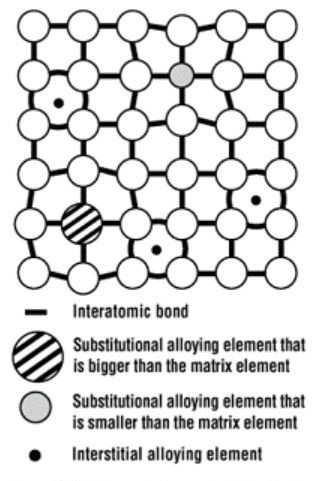
\includegraphics[width=.5\textwidth]{small_gaps_between_atoms.jpg}
    \caption{Small gaps between atoms, called “interstices” (\cite{bajaj2020steels}).}
    \label{ch3:figure:gaps}
\end{figure}

\begin{figure}[H]
    \centering
    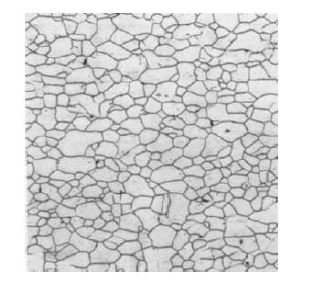
\includegraphics[width=.5\textwidth]{microstructure_of_carbon_steel.jpg}
    \caption{Microstructure of fully ferritic, ultralow carbon steel. Marshalls etch + HF, 300x (\cite{molabe2018determining}).}
    \label{ch3:figure:microstructure}
\end{figure}

 Since the carbon elements have occupied the interstices, larger elements such as manganese, magnesium, silicon, and phosphorus substitute for iron in the lattice, (see Figure \ref{ch3:figure:tank}) (\cite{jones2012engineering}).  However, there is a limitation on how much carbon can occupy the interstices. Commonly, 0.02\% carbon at 725 ℃, but dropping to 0.006\% carbon at room temperature is more than enough to fit in the interstices (\cite{bhadeshia2017steels}). Ferrite has a bcc crystal structure with a microstructural phase that is soft, ductile, which is similar to pure iron (\cite{bajaj2020steels}). The microstructure of ferrite is shown in Figure \ref{ch3:figure:microstructure}.

\subsection{Austenite} 
In the phase known as austenite, the interstices are much larger than in the ferrite phase and have the \acrshort{fcc} crystal structure, as shown in Figure \ref{ch3:figure:austenite} (\cite{bajaj2020steels}). This allows more carbon content to occupy the interstices. At critical temperatures, which is around 1,150 ℃, carbon content up to 2\% can fit into the austenite, as the result of larger interstices (\cite{bhadeshia2017steels}). As a consequence, in plain-carbon and low alloy steels, the austenite phase is not possible to form at room temperature but can only exist in relatively small amounts of retained austenite that was unable to transform during the rapid cooling process (\cite{molabe2018determining}).

\begin{figure}[H]
    \centering
    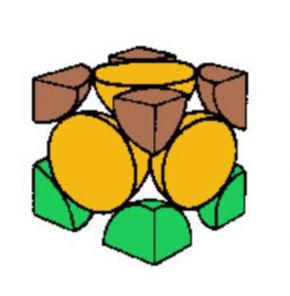
\includegraphics[width=.5\textwidth]{austenite_fcc_crystal_structure.jpg}
    \caption{An austenite FCC crystal structure (\cite{bajaj2020steels}).}
    \label{ch3:figure:austenite}
\end{figure}

Since the austenite phase is not possible to form at room temperature for the lowest alloy steels, then their properties are also affected. Consequently, austenitic steels usually suffer from stress-corrosion cracking and low yield strength. Moreover, their strengthening processes are limited to only cold working, interstitial solid-concentrate strengthening, or precipitation hardening (\cite{molabe2018determining}). However, \acrshort{fcc} alloy has low-temperature toughness, excellent weldability, and resistance to corrosion (\cite{bhadeshia2017steels}).


\subsection{Pearlite}
When the largest amount of carbon has occupied the interstices to form austenite at the critical temperature, the steel gradually cools at eutectoid temperature (723℃) on the iron-iron carbide equilibrium diagram, shown in Figure \ref{ch3:figure:equilibrium}. Thus, the carbon content is forced out of the concentrate  (\cite{bhadeshia2017steels}). During this cooling process, the austenite transforms into a combination of ferrite and another phase known as cementite, also known as iron carbide, which has the chemical composition of Fe3C (\cite{cmrp2014maintenance}). The combination of ferrite and cementite is known as \emph{pearlite}.

For plain carbon steels, ferrite, cementite, and pearlite phases are the principal constituents of the microstructure, provided that they have been cautiously subjected to slow cooling to avoid the formation of the metastable phases. Consequently, it is significant to evaluate the nucleation and growth of these phases and to determine the factors which control their morphology (\cite{bhadeshia2017steels}).

Cementite on its own has characteristics of ceramic materials, very hard and brittle, with low toughness and little resistance to crack initiation and propagation, which is unlike ferrite (\cite{bajaj2020steels}). As a result, pearlite may reveal more than one microstructure due to the alternating layers of ferrite and cementite. A fully pearlitic microstructure is significantly formed at the eutectoid composition of 0.78\%C, as shown in Figure \ref{ch3:figure:equilibrium} (\cite{molabe2018determining}).
\begin{figure}[H]
    \centering
    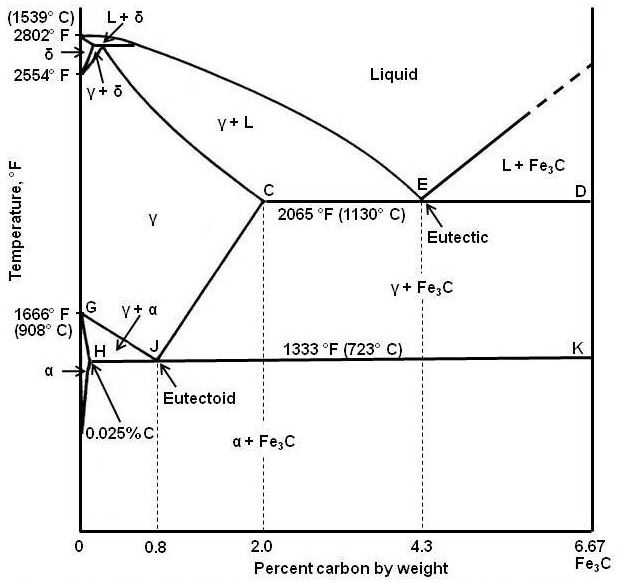
\includegraphics[scale=0.87]{iron-iron_carbide_equilibrium_diagram.jpg}
    \caption{Iron-iron carbide equilibrium diagram showing the austenite ($\gamma$), ferrite ($\alpha$) and cementite (Fe3C) phase regions with eutectoid composition and temperature (\cite{cmrp2014maintenance}).}
    \label{ch3:figure:equilibrium}
\end{figure}
\begin{figure}[H]
\centering
\begin{subfigure}{.45\textwidth}
    \centering
    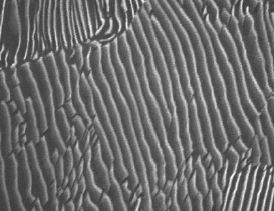
\includegraphics[height=5cm,width=\textwidth]{ferrite_and_cementite_lamellae_micrograph.jpg}
    \caption{}
\end{subfigure}
\begin{subfigure}{.45\textwidth}
    \centering
    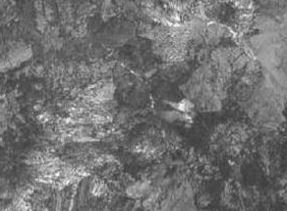
\includegraphics[height=5cm,width=\textwidth]{fully_pearlitic_steel.jpg}
    \caption{}
\end{subfigure}

\caption{Pearlite microstructures:  SEM micrograph of pearlite showing ferrite and cementite lamellae. 4\% picral etch. 10000x a). Fully pearlitic steel showing the characteristic fine pearlite interlamellar spacing. 2\% nital + 4\% picral etch. 500x b) (\cite{molabe2018determining}).}
\label{ch3:figure:pearlite:microstructures}
\end{figure}

 In contrast to cementite, fully pearlitic steels have high strength, high hardness, and good wear resistance. However, they commonly suffer from poor ductility and poor toughness (\cite{molabe2018determining}). Figure \ref{ch3:figure:pearlite:microstructures} shows a microstructure fully pearlite steel and pearlite showing ferrite and cementite lamellae.


\subsection{Ferrite-Pearlite}
Ferrite-pearlite is the common microstructural phase that makes the plainest carbon steel. The microstructure and properties of these steels are distinguished, usually by the carbon content present and the size of the grains, as shown in Figure \ref{ch3:figure:austenite} (\cite{molabe2018determining}). However, as previously stated in Section \ref{ch3:anchor:section:morphology}, carbon content has an impact on some properties of steel, thus it has a strong relationship with the tensile strength of ferrite-pearlite steels. As illustrated in Figure \ref{ch3:figure:properties}, carbon content has a direct relationship with the ultimate strength of ferrite-pearlite steels due to the gradual increase of ultimate tensile strength as a function of carbon content (\cite{zhao2013effects}).

\begin{figure}[H]
\centering
\begin{subfigure}{.49\textwidth}
  \centering
 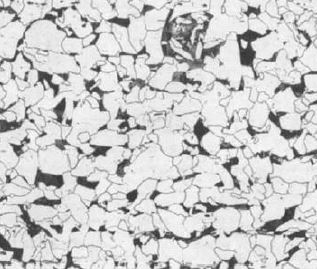
\includegraphics[height=1.0\textwidth, width=\textwidth]{ferrite-pearlite_carbon_content_1.jpg}
 \caption{}
\end{subfigure}
\begin{subfigure}{.49\textwidth}
 \centering
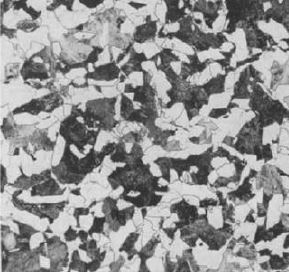
\includegraphics[height=1.0\textwidth, width=\textwidth]{ferrite-pearlite_carbon_content_2.jpg}
\caption{}
\end{subfigure}

\caption{Microstructure of typical ferrite-pearlite steels at two different carbon contents: 0.10\% C (a) and 0.25\% C (b). 2\% nital + 4\% picral etch. 200x (\cite{osei2015foam}).}
\label{ch3:figure:contents}
\end{figure}


Pearlite has more carbon content on the microstructure, thus this is the main reason for the increase in the ultimate strength of ferrite-pearlite steels (\cite{bajaj2020steels}). Consequently, the strength of pearlite is much higher than that of ferrite (\cite{molabe2018determining}). In contrast, the yield strength of ferrite-pearlite steels is not dependent upon the carbon content. However, the ferrite matrix commonly governs the yielding in ferrite-pearlite steels. The Ferrite matrix is regarded as a repeating phase in the microstructure of ferrite-pearlite, hence pearlite alone has a slight effect on the yielding behaviour (\cite{molabe2018determining}). Figure \ref{ch3:figure:contents} shows the microstructure of ferrite-pearlite steels at two different carbon contents, to further understand the effect of carbon on steels. 
  
\begin{figure}[H]
    \centering
    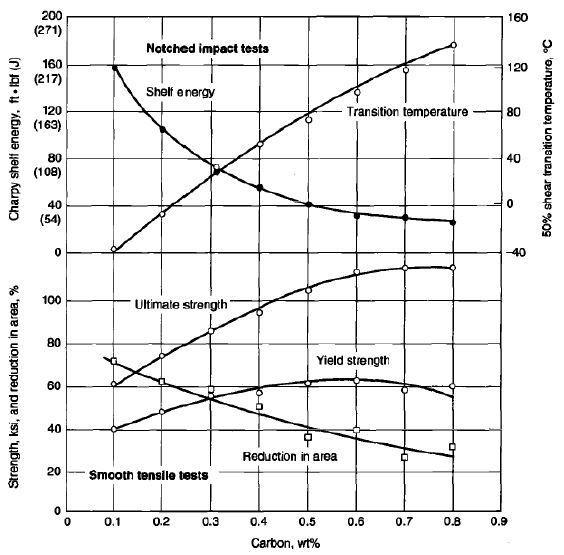
\includegraphics[scale=1]{mechanical_properties_of_ferrite-pearlite_steels.jpg}
    \caption{Mechanical properties of ferrite-pearlite steels, as a function of carbon content (\cite{molabe2018determining}). }
    \label{ch3:figure:properties}
\end{figure}

\subsection{Martensite}
Martensite is a supersaturated solid concentrate of carbon in iron (\cite{molabe2018determining}). It is generally formed during the rapid cooling process when the waste carbon of the fcc austenite does not have time to diffuse out of the crystal structure and form cementite (\cite{bajaj2020steels}). Instead, the carbon content is 'trapped' in with the now almost pure iron, and is relatively forced into interstitial locations that are not large enough to accommodate the carbon atoms. Consequently, this distorts and strains the crystal matrix into a body-centred tetragonal (bct) structure, as shown in Figure \ref{ch3:figure:martensite}. Thus this forms a very hard phase known as martensite (\cite{molabe2018determining}).
 
\begin{figure}[H]
    \centering
    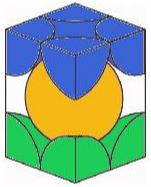
\includegraphics[width=.25\textwidth]{bct_crystal_structure_of_martensite.jpg}
    \caption{A bct crystal structure of martensite, which has larger gaps within the unit cell (\cite{bajaj2020steels}).}
    \label{ch3:figure:martensite}
\end{figure}

When the content of carbon is constantly increasing to higher levels, more carbon is frozen into the bct structure, further straining the crystal matrix. Thus this is the main reason for the hardness of martensite to increase a function of carbon content (\cite{bajaj2020steels}). In addition, the volume of the bct martensite structure is larger than that of the fcc austenite. Consequently, the transformation of fresh martensite is significantly compressed by the surrounding matrix (\cite{bajaj2020steels}). A typical microstructure of martensite is shown in Figure \ref{ch3:figure:martensite:microstructures}.

The hardness of martensite can be significantly reduced by further heating the martensite. In such cases, the carbon content has the opportunity to diffuse out from the bct structure, reducing the distortion of the crystal matrix in that process, and thus reducing the hardness and increasing the toughness (\cite{bhadeshia2017steels}). However, after the heat treatment process, the microstructure of ferrite and iron carbide is formed, which leads to the formation of \emph{tempered martensite} (\cite{bajaj2020steels}). Since the martensitic matrix is strained, it results in an increased amount of iron carbide nucleation sites in tempered martensite, which eventually leads to a more widespread distribution of iron carbide than seen in the lamellar (layered) structure of pearlite, shown in Figure \ref{ch3:figure:microstructure} (\cite{bajaj2020steels}). The bcc ferrite has a smaller volume compared to bct martensite, thus when martensite is tempered, some of the remaining martensite compression stresses from the austenite-to-martensite transition are mitigated (\cite{molabe2018determining}).

\begin{figure}[H]
\centering

\begin{subfigure}{.45\textwidth}
    \centering
    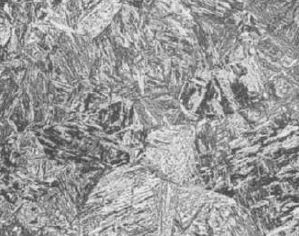
\includegraphics[height=6cm, width=\textwidth]{lath_martensite_microstructure.jpg}
    \caption{}
\end{subfigure}
\begin{subfigure}{.45\textwidth}
    \centering
    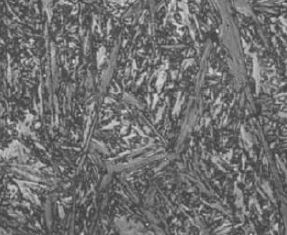
\includegraphics[height=6cm, width=\textwidth]{plate_martensite_microstructure.jpg}
    \caption{}
\end{subfigure}

\caption{Martensite microstructures: a typical lath martensite (a) and a plate martensite (b). 4\% picral + HCl. 200x (\cite{molabe2018determining}).}
\label{ch3:figure:martensite:microstructures}
\end{figure}

\subsection{Bainite}
Bainite is another possible microstructure that can form when austenite is cooled. It is typically a mixture of ferrite, cementite, and retained austenite. However, ferrite has an acicular morphology and the carbides are discrete particles, which is the main difference from the pearlite microstructure (\cite{molabe2018determining}). \emph{Retained austenite} is the term given to austenite that does not transform to martensite during quenching (\cite{bajaj2020steels}). The cooling rate required to form bainite is much slower compared to the cooling rate needed to form martensite. As a consequence, carbon has the opportunity to diffuse out of the fcc austenite, thus allowing the formation of the \acrshort{bcc} ferrite.

Bainitic microstructures have an excellent balance in terms of strength and ductility, which is useful in many applications. These are the results of a sufficient cooling rate that significantly increases the strength. The higher cooling rates required to produce bainite give the harder components of the microstructure enough energy to transform into a more rounded shape (\cite{bajaj2020steels}). In this way, the hard microstructural constituents do not easily suffer crack initiation and propagation as compared to flat and elongated ones.
     
\begin{figure}[H]

\centering
\begin{subfigure}{.45\textwidth}
    \centering
    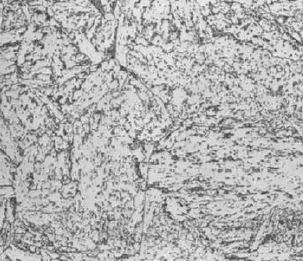
\includegraphics[height=.9\textwidth, width=\textwidth]{upper_bainite_microstruce.jpg}
    \caption{}
\end{subfigure}
\begin{subfigure}{.45\textwidth}
    \centering
    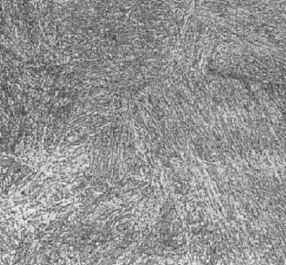
\includegraphics[height=.9\textwidth, width=\textwidth]{lower_bainite_microstructure.jpg}
    \caption{}
\end{subfigure}

\caption{Bainite microstructures: upper bainite (a) and lower bainite (b), in Cr-Mo-V rotor steel. 2\% nital + 4\% picral etch. 500x (\cite{molabe2018determining}).}
\label{ch3:figure:bainite:microstructures}
\end{figure}

Normally bainite has two morphologies, namely, upper bainite and lower bainite, which are shown in Figure \ref{ch3:figure:bainite:microstructures}. These two morphologies depend upon the temperature regions at which bainite was formed during the isothermal transformation (\cite{molabe2018determining}). The upper bainite is typically formed isothermally in the temperature range of 400-550 ℃, while lower bainite is also formed by an isothermal process in the temperature range of 250-400 ℃ (\cite{molabe2018determining}). Consequently, the iron carbide phase critically forms at the lath boundaries in upper bainite, while the carbide phase forms on certain crystallographic planes within the laths in lower bainite (\cite{bajaj2020steels}). The lower bainite has higher strength and higher toughness compared to the upper bainite due to the fine acicular structure and the carbides within the laths. Generally, lower bainite has higher strength and higher toughness compared to upper bainite. This is due to the fine acicular structure and carbides possessed by lower bainite within the laths (\cite{molabe2018determining}).

\subsection{Ferrite-Cementite}
When plain carbon steels are heated to temperatures slightly below the lower critical temperature, a ferrite-cementite microstructure that has a spheroidized shape as shown in Figure \ref{ch3:figure:spheroidized_steel} is significantly formed (\cite{molabe2018determining}). However, the spheroidized structure is commonly revealed after the formation of pearlite. During the spheroidization, the cementite lamellae of the pearlite change their morphology to result to form spheroids (\cite{molabe2018determining}).

\begin{figure}[H]
    \centering
    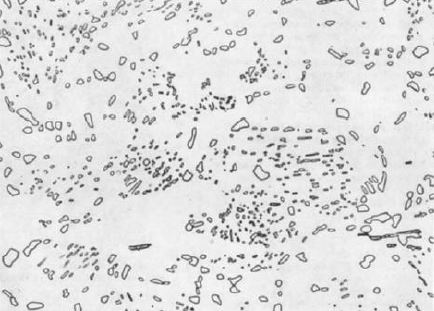
\includegraphics[width=.6\textwidth]{microstructure_of_fully_spheroidizel_steel.jpg}
    \caption{Microstructure of fully spheroidized steel. 4\% picral etch. 100x (\cite{molabe2018determining}).}
    \label{ch3:figure:spheroidized_steel}
\end{figure}

The critical and controlling factors during this process are the The critical and controlling factors during this process are the diffusion of carbon and portions of lamellae that should significantly dissolve and then diffuse to yield the formation of a spheroid from the remaining portions of lamellae (\cite{molabe2018determining}). The ferrite-pearlite phase has several benefits in terms of the resulting properties. For example, fully spheroidized structures normally have enhanced machinability properties for most plain carbon steels (\cite{molabe2018determining}).  The machinability of steels is one of the vital properties in the present study thus the formation of ferrite-cementite should be thoroughly evaluated and assessed.

\subsection{Ferrite-Austenite}
The ferrite-austenite are the two phases that are present in duplex stainless steels, see Figure \ref{ch3:figure:steel_phase}. The proportion of these two phases in duplex stainless steels in relatively equal. The duplex stainless steels can be altered to a completely ferritic structure. This is possible when they are melted and solidifies from the liquid phase (\cite{xiao2006challenge}).  However, as the materials significantly cool to room temperature, about half of the ferritic grains transform into austenitic grains (\cite{davison1991guide}). Figure \ref{ch3:figure:duplex_microstructure} shows a combination of ferrite and austenite phases that forms one microstructure.

The combination of ferrite and austenite structures yields several attractive properties. Consequently, duplex stainless steels are about twice as stronger compared to regular austenitic and ferritic stainless steel (\cite{davison1991guide}). The ductility of duplex steels is relatively fair, they, however, do not reach the excellent values of austenitic grades due to the different levels of nickel (\cite{molabe2018determining}). Stress corrosion resistance is another property that has made duplex stainless steels to be the most extensively utilized family of stainless steels. 

\begin{figure}[H]
    \centering
    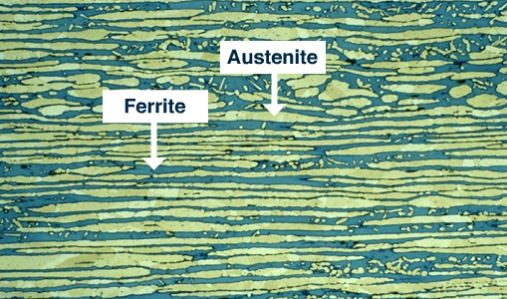
\includegraphics[width=.6\textwidth]{duplex_microstructure_that_has_yellow_austenitic_phase.jpg}
    \caption{Duplex microstructure that has yellow austenitic phase as “islands” surrounded by the blue ferritic phase (\cite{davison1991guide}).}
    \label{ch3:figure:duplex_microstructure}
\end{figure}

\section{Characterization of defects} 
While the microstructure of steels critically determines the resulting properties, they may still have a variety of imperfections known as defects and discontinuity. Both material discontinuity and crystal defects have diverse effects on the deformation behaviour and some of the physical and chemical properties of steels (\cite{suryanarayana2017microstructure}). Hence it is of great significance to determine the nature and quantity of the crystal defects present in a steel material. 

Numerous methods have been extensively utilized to characterize the defects in steel. However, according to some researchers, the \Acrfull{tem} technique is more suitable to characterize defects on steels (\cite{george2002introduction, bhadeshia2017steels}). Besides, the \acrshort{tem} method has been proven to be reliable on numerous occasions. In any metallic material crystal defects can occur, these defects may include, point defects (vacancies, interstitial atoms), line defects (dislocations), planar defects (stacking faults, twin boundaries), and volume defects (voids, cavities). One of the objectives of the present study is to improve the properties of steels based on the understanding of microstructure morphology. Thus, the characterization of vacancies and dislocation defects is also of interest.

\subsection{Vacancies} 
 In almost every instance, individual vacancies cannot be seen on \acrshort{tem}, due to the size and complications that are usually encountered. However, their aggregation into voids, resulting in the formation of dislocation loops in quenched steels, helps in estimating the vacancy concentration. In this way, the dislocation loops are significantly characterised, which then makes it possible to determine whether they are formed from vacancy condensation or interstitial atoms (\cite{suryanarayana2017microstructure}).

\subsection{Dislocations}
This defect is commonly divided into two types, screw and edge dislocation. The complications arise when characterizing the type of dislocation that is present in steels (\cite{jones2012engineering}). However, this is conveniently achieved by using the extinction (invisibility) criterion \textbf{g.b} = 0, where \textbf{g} is the reciprocal lattice vector, and \textbf{b} is the burgers vector. By properly orientating the specimen, a dislocation will become invisible, and this can occur at more than one \textbf{g} value. The equation can nonetheless be manipulated by simply putting the determination of two (or more) of these \textbf{g} values, which then enables calculating \textbf{b} (\cite{suryanarayana2017microstructure}).

Many experimental studies have been conducted to ease and improve the characterization of crystal defects (\cite{george2002introduction, bhadeshia2017steels, karayan2014weld}). Despite this, Suryanarayana \cite{suryanarayana2017microstructure} validated that \acrshort{tem} remains a suitable technique for characterizing crystal defects in steels. Moreover, \acrshort{tem} enables the determination of disorientation between grains (for both low-angle and high-angle grain boundaries), the fault vector in stacking faults, the extent of coherency, or incoherency between two phases, the sizes and volume fractions of precipitates, and many other features (\cite{suryanarayana2017microstructure}).

\section{Effects of heat treatment on steels}
\label{ch3:anchor:section:treatment}
Heat treatment is an industrial process that is commonly used to improve the existing properties of metals, especially steels. To be precise, it is often used to enhance mechanical, physical, and sometimes chemical properties (\cite{mampuya2021effect}). The heat treatment process modifies the microstructure of the steel, thus altering the resulting properties. The role of each microstructural constituent is comprehensively presented in Figure \ref{appendix:role} on appendices. In recent years several methods have been developed to enhance the properties of engineering materials, especially for liquid storage facilities. Approaches like thermochemical and thermomechanical are examples of such techniques (\cite{singh2020applied}). However, the heat treatment process has been a sensible approach for the optimization of steel properties.

Normally, the first step in the heat treatment of steel is to effectively heat the steel to some temperature at or above the critical range to form austenite (\cite{mampuya2021effect}). However, to fully comprehend the heat treatment process of steels, it is crucial to first understand the phase diagram for the steel of interest. Heat treatment comprises several subsequent processes that are all critical. Various heat treatments are normally based on the subsequent cooling and reheating of the austenitized steel (\cite{singh2020applied}).  For the present research work, only the relevant heat treatment processes will be discussed.

\subsection{Annealing}
The ductility of steel or any metallic material is normally enhanced by the annealing process. This process involves heating the steel to a predetermined temperature and then slowly cooling it to room temperature in a furnace (\cite{singh2020applied}). However, enhancing the ductility of the steel results in a reduction in brittleness. Sometimes annealing process can be utilized to improve the machinability of steels (\cite{nikkhah2019improved}). As a consequence, annealing is a vital process for liquid storage facilities due to the demand for ductility and ease of machinability during the fabrication process. The full annealing temperature cycle is shown in Figure \ref{appendix:range} on appendices, which includes the hardness range on steel after annealing. 

Annealing is a broad process that involves several thermal cycles, which are classified based on the maximum level of temperature reached during the heating of the steel (\cite{singh2020applied}). The thermal cycles usually involve subcritical, inter critical, and full annealing. Appendix 2.1 indicates the recommended temperatures and cooling cycle for full annealing of various carbon steel forgings (\cite{singh2020applied}).

\subsection{Normalizing}
The purpose of normalizing is very broad and normally depends upon the history of the steel, the cycle of heating, and cooling practised. However, this process is commonly used to achieve the desired hardness and strength of the steel (\cite{singh2020applied}). Therefore, it can increase or decrease these properties, depending on the objectives. 

Normalizing is sometimes known for overlapping the function of other types of heat treatments, such as annealing, hardening, and stress relieving (\cite{singh2020applied}). This is due to multiple properties it normally improves simultaneously, which can be individually achieved by each other heat treatment processes. Normalising can produce harder and stronger steel and also improves machinability (\cite{mampuya2021effect}). However, in the normalizing process, the cooling is not performed under equilibrium conditions, thus there are often deviations from the phase diagram predicted structures (\cite{singh2020applied}).  For steels that are normally used for the construction of liquid storage facilities, normalizing is essential to achieve the desired strength and hardness, as well as improved machinability.

\subsection{Tempering}  
Almost all steels are too brittle in the quenched martensitic condition for most applications, especially storage facilities. This is due to high residual stresses that are commonly induced as the result of martensite transformation (\cite{mampuya2021effect}). Consequently, tempering always follows the hardening or normalizing process to relieve the residual stresses and relax the steel. 

Tempering is a heat treatment process that involves heating the steel to a temperature below the lower critical temperature (\cite{singh2020applied}). This results in relieving the residual stresses, and enhancement of the ductility and toughness of the steel. In most heat treatment processes, there is usually a sacrifice of other properties to obtain others. As a consequence, in the tempering process, there is a sacrifice of hardness and strength. As the tempering temperature is constantly increased, the hardness decreases, while the toughness increases (\cite{singh2020applied}). Various types of tempering are known to date, austempering and martempering are the commonly used processes.

\subsection{Quenching}  
The rate of cooling of any metallic material is vital and has an impact on the resulting properties. Quenching is the process of cooling the steel, usually at a rapid rate, to produce a martensitic transformation (\cite{singh2020applied}). The rate of cooling has different effects on different metals, in ferrous alloys, the rapid rate will result in a harder metal, while in non-ferrous alloys, a softer metal will be produced (\cite{mampuya2021effect}). The rapid rate of cooling usually hardens steel. Therefore, in order to achieve softer steel, a slower rate of cooling should be applied. However, this, of course, varies with the type of steel. 

Quenching can be achieved in numerous ways, commonly by forced air or other types of gases. Liquids such as water and oil can also be utilized to quench steels due to their better thermal conductivity (\cite{singh2020applied}). There are three stages of cooling during the quenching process, and all are closely related to the cooling medium being used. Vapour is the first quenching medium that is applied to the steel surface, and during this stage, the cooling process is relatively slow. When the metal has cooled enough, and the vapour film is no longer stable, the second stage then takes place, which is wetting the surface of the steel. This is usually the rapid stage of cooling the steel. Finally, liquid cooling commences when the surface temperature of the steel finally reaches the boiling point of the liquid to halt the formation of vapour (\cite{marzorati2018green, protopopoff2011surface}). However, this is commonly the slowest stage of cooling.

Recently, most researchers have been interested in understanding the relationship between heat treatments, microstructure, and mechanical properties (\cite{marzorati2018green, whitman1924effect, cai2018influence}). \cite{mampuya2021effect} investigated the effect of heat treatment on the microstructure of duplex stainless steel 2205. They further reported that the transition of austenite and ferritic phases often results in critical changes in the hardness of the specimen when air-cooled. While there is a slight change in the hardness when it is water or oil-cooled. \cite{zhang2021influence} conducted an experimental study to understand the effect of slow-cooling heat treatment on the mechanical properties of high-strength steels. Their results indicated that the slow-cooling heat treatment can effectively reduce the yield and ultimate strengths of high-strength steels. \cite{essoussi2019heat} reported that the strength and elongation of AISI 304 austenitic stainless steels can be improved by quenching without tempering, while the hardness will relatively decrease during this process.

There is a lack of research on the effect of heat treatment on the corrosion properties of steel. However, some researchers have made a significant effort to thoroughly understand the relationship between corrosion and heat treatment processes (\cite{whitman1924effect, hackerman1987theory}). The corrosion resistance of steel is largely dependent upon the composition and microstructures (\cite{wang2020enhancing}). The microstructures could nonetheless be improved by the process of heat treatment. \cite{sarkar2020effects} investigated the effect of heat treatment on the microstructure, mechanical, and corrosion properties of stainless steel. The study showed that the retained austenite is more for specimens without solution annealing, which increases the tensile strain and decreases the hardness and wear rate. To enhance the corrosion resistance of martensite stainless steel, \cite{wang2020enhancing} conducted numerous experiments and they reported that the austenite phase disappears and new duplex particles accelerated after concentrate treatment and aging treatment, which decreased the pitting corrosion. 

One of the objectives of the present research work is to improve the corrosion resistance of duplex stainless and mild steels in a corrosive atmosphere. Consequently, all these previous studies and relevant literature is used as a benchmark for the present study. Experimentally and theoretically, they provide comprehensive guidance in terms of optimizing the materials used for constructing \acrshort{afff} storage facilities.

\section{Polyethylene plastics}
Plastics also known as polymers have become a major class of engineering materials. Polymers are substances whose molecules have high molar masses and are composed of a relatively large number of repeating units. There are both naturally occurring and synthetic polymers (\cite{roslan2013effect}). They offer several beneficial properties (mechanical, physical, chemical and optical) when utilised for certain industrial applications (\cite{nugent2017rotational}). In contrast to metals, polymers are generally characterised by lower density, strength, elastic modulus, thermal and electrical conductivity, high corrosion resistance, and cost (\cite{roslan2013effect}). Thus, this is the reason for the rapid increase in plastic processing on annual basis. In addition, they are the preferred materials over metals nowadays for numerous industrial applications. However, their setback to date is they are a waste that affects the environment if no longer in use. Nonetheless, there have been developments over the years that are aiming to rectify this issue, with the notable one being recycling.  

Many plastic materials fall under the polymer tree. However, for the present study polyethene (\acrshort{pe}) plastics will be discussed. This is due to the growing demand for this material for manufacturing liquid storage facilities. \acrshort{pe} is undoubtedly the most popular plastic material in the world. It is a commodity material, which statically accounts for about 70\% of the plastic family (\cite{roslan2013effect}).  \acrshort{pe} is thermoplastic in nature and therefore it can be reprocessed repeatedly, thus this is the reason it is easily available at a relatively low cost and can be easily processed (\cite{kurtz2009cross}). Moreover, it can be utilised for diverse industrial applications. 

\acrshort{pe} is often classed by the density it contains. Therefore, there is a \Acrfull{ldpe} ($0.910 < density < 0.925$), \Acrfull{mdpe} ($0.926 < density < 0.940$), and \Acrfull{hdpe} (\cite{gabriel1998history}). Consequently, changing the density of the \acrshort{pe} will result in altering the properties. The effect of changes in density, melt index, and molecular weight distribution on the properties of \acrshort{pe} are tabulated in Figure \ref{appendix:classifications} on appendices.

\acrshort{hdpe} is commonly used in the manufacturing of chemical or liquid storage facilities, due to the seamless final product that is produced, for greater strength and corrosion resistance, thus it is of great importance in the present study. \acrshort{hdpe} is a thermoplastic material composed of mainly carbon and hydrogen atoms joined together to form a high molecular weight product as shown in Figure \ref{ch3:figure:molecular_chains} (\cite{gabriel1998history}). Methane gas is converted into ethylene then, with the application of heat and pressure it is further converted to polyethene. The polymer chain may be 500,000 to 1,000,000 carbon units long. The longer the main chain, the great the number of atoms (\cite{gabriel1998history}). As expected, the properties of \acrshort{hdpe} or any plastic material depend upon the arrangement of the molecular chains.
               
\begin{figure}[H]
\centering

\begin{subfigure}{.3\textwidth}
    \centering
    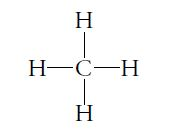
\includegraphics[width=\textwidth]{methane_molecular_chain.jpg}
    \caption{Methane}
\end{subfigure}
\begin{subfigure}{.3\textwidth}
    \centering
    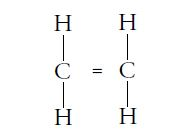
\includegraphics[width=\textwidth]{ethylene_molecular_chain.jpg}
    \caption{Ethylene}
\end{subfigure}
\begin{subfigure}{.65\textwidth}
    \vspace{1.5em}
    \centering
    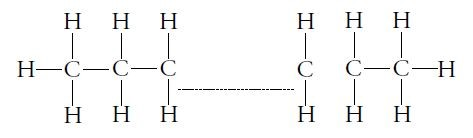
\includegraphics[width=\textwidth]{polythylene_molecular_chain.jpg}
    \caption{Polyethylene molecular chain}
\end{subfigure}

\caption{a) Methane gas, b) ethylene and c) polyethylene (\cite{gabriel1998history}).}
\label{ch3:figure:molecular_chains}
\end{figure}

\subsection{Cross-linked polyethylene (XLPE) material}
Many researchers have been making efforts in obtaining a \acrshort{pe} with specific chemical, mechanical, and thermal characteristics for the fabrication of complex-shaped products, or for use in adverse environmental conditions (\cite{kurtz2009cross}). In general, plastic is a light and weak substance that easily melts when exposed to heat. However, altering the carbon atoms within the structure changes this perspective. To be precise, cross-linking the carbon atoms within the structure usually transforms such material into a superior material that may be resistant to temperature, pressure, and corrosion, and that can be used in a variety of applications (\cite{peacock2000handbook}). Crosslinking is known as a process in which carbon atoms of the same or different polyethene chains are joined together to form a three-dimensional network structure (\cite{kurtz2009cross}).

The crosslinking technique was first discovered in the late 1960s by the European scientist known as Engel (\cite{peacock2000handbook}). The introduction of cross-linked polyethene (\acrshort{xlpe}) was another milestone in the plastic era. As a consequence, when \acrshort{pe} is cross-linked, it is advantageously employed in the manufacturing of storage facilities due to the advanced resulting properties. The fundamental way to enhance material properties such as impact strength, chemical resistance, and thermal characteristics is via cross-linking (\cite{andreopoulos1986mechanical}). Cross-linking will however change the nature of the polymer from thermoplastic to thermosetting polymer, thus yielding a non-melting and more durable polymer matrix (\cite{clemens2017microstructure}). Crosslinking method is easily achieved in branched polymers. From the branched \acrshort{hdpe} it is convenient to crosslink the polymer. However, this is a long and tiring process as compared to \acrshort{ldpe}.

Since \acrshort{hdpe} has a linear molecular structure, therefore crosslinking this type of polymer requires special attention as compared to \acrshort{ldpe}. Figure \ref{ch3:figure:hdpe} and \ref{ch3:figure:ldpe} shows the process of branching \acrshort{hdpe} and \acrshort{ldpe} respectively.
 
\begin{figure}[H]
    \centering
    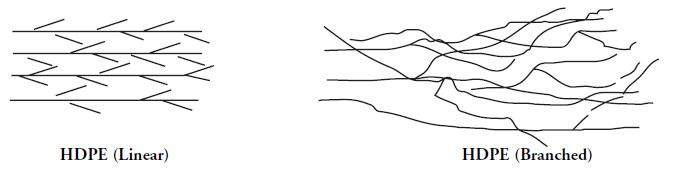
\includegraphics[width=\textwidth]{linear_and_branched_hdpe.jpg}
    \caption{Linear and branched HDPE (\cite{gabriel1998history}).}
    \label{ch3:figure:hdpe}
\end{figure}

\begin{figure}[H]
    \centering
    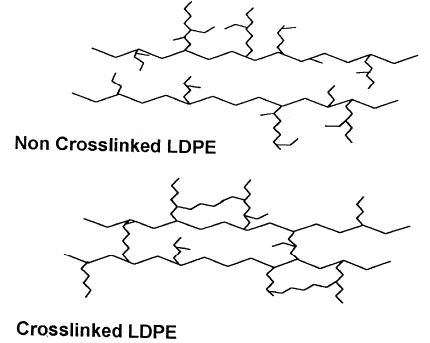
\includegraphics[width=.6\textwidth]{crosslinked_and_non_crosslinked_ldpe.jpg}
    \caption{Crosslinked and non-crosslinked LDPE (\cite{kurtz2009cross}).}
    \label{ch3:figure:ldpe}
\end{figure}

\begin{figure}[H]
    \centering
    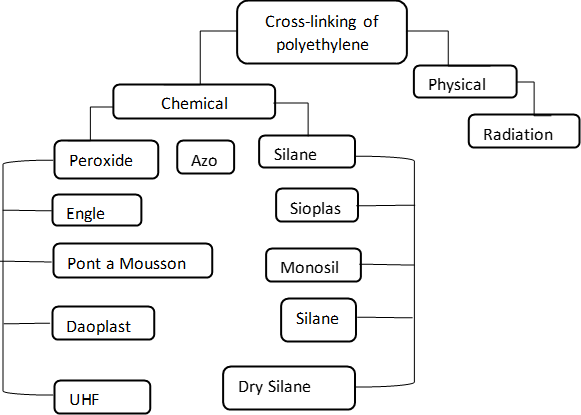
\includegraphics[width=.95\textwidth]{methods_available_for_crosslinking_polyethylene.png}
    \caption{Methods available for crosslinking polyethylene (\cite{patterson2022cross}).}
    \label{ch3:figure:crosslinking_methods}
\end{figure}

Over the past decades, there have several crosslinking methods that have been developed. However, to date, two tested methods are used to crosslink polymers, chemical and radiation (physical) methods (\cite{clemens2017microstructure, bajaj2020steels}). These two methods are unique in their way and are often utilized for a specific purpose. They usually depend upon the state (molten or solid) of the polymer during crosslinking and the type of activator used to promote crosslinking (\cite{kurtz2009cross}). Figure \ref{ch3:figure:crosslinking_methods} illustrates the available crosslinked methods in detail, as discussed above.

\subsubsection{Chemical processes}
This is an extensively used method for crosslinking polymers. For the method to work as desired, a chemical substance usually peroxide or silane is required to significantly activate the links in the polymer chain, thus it is known as a chemical process (\cite{peacock2000handbook}). During the chemical process, crosslinking takes place through direct carbon-to-carbon bonds. An alternative may be through the chemical bridges that connect various polyethene molecules (\cite{kurtz2009cross}). 

In recent years, most researchers have been interested in knowing the crosslinking method that yields quality thermoplastic. The recent relevant literature suggests that the intensity of crosslinking in thermoplastic resin usually varies with the crosslinking process. Chemical crosslinking using peroxide significantly results in the highest and most uniform degree of crosslinking as compared to the radiation process (\cite{clemens2017microstructure, bajaj2020steels}). \cite{peacock2000handbook} experimentally investigated the difference in the degree of crosslinking polymers using chemical and radiation processes. The outcome was that radiation crosslinking yields between 34-75\% degree of crosslinking. In the chemical crosslinking method, peroxide gives a much higher degree of crosslinking (up to 90\%), while silane-based crosslinking can be 45-70\% degree of crosslinking.

\paragraph{Peroxide processes} \hfill \\
Peroxide crosslinking process has been utilised for nearly over 40 years and is the most common crosslinking process of thermoplastics, especially polyethene. In this method, the organic peroxide is used as the initiator. In most cases, an organic peroxide is used its original unprocessed structure (\cite{peacock2000handbook}). It is important to note that this process only occurs when the thermoplastic is in a molten state. In addition, the process is a carbon-based chemical that includes a minimum of two oxygen atoms that are bonded together (-O-O-). The general formula is:

 \begin{equation}
    R^1-O-O-R^2
 \end{equation}

Where, R1 and R2 values can be aryl, alkyl, or acyl groups and O being the two oxygen atoms which are bonded together. The alkyl peroxides significantly produce the most reactive free radicals; thus, they are the most used peroxides for crosslinking (\cite{kurtz2009cross}). Figure \ref{ch3:figure:crosslinking_process} shows the entire schematic representation of crosslinking polyethene using the peroxide substance. The peroxide process has the advantage of producing high thermal stability products due to the C-C bonds, however, this is achieved at relatively high costs (\cite{patterson2022cross}).

\begin{figure}[H]
    \centering
    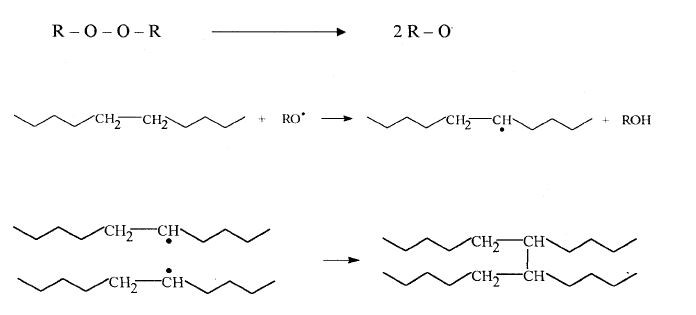
\includegraphics[width=.9\textwidth]{process_of_crosslinking_using_the_organic_peroxide_as_the_initiator.jpg}
    \caption{Process of crosslinking using the organic peroxide as the initiator (\cite{peacock2000handbook}). }
    \label{ch3:figure:crosslinking_process}
\end{figure}

\paragraph{Silane processes} \hfill \\
For this process to be possible, crosslinking is significantly activated by silane coupling agents, which react with many chemicals, including polymers, through typical organic chemistry reactions. The organ silane molecule critically includes a central silicon atom (Si) bounded to two different categories of groups (vinyl and alkoxy), which usually displays different reactivity (\cite{kurtz2009cross}). Both these groups are vital in the process of cross-linking. The vinyl groups usually allow silane grafting to the \acrshort{pe} and alkoxy groups generate a three-dimensional network of siloxane linkages in the presence of water or moisture (through condensation or hydrolysis).

In contrast to the peroxide process, the \acrshort{pe} is cross-linked in the crystalline state in the silane process. Thus, the uses of silanes result in the formation of siloxane (Si-O-Si) bridges, which are less rigid than carbon-to-carbon (C-C) bonds produced in the peroxide process. The silane process is shown in Figure \ref{ch3:figure:reaction} in a two-step process, starting from the grafting of silane on \acrshort{pe} to condensation (cross-linking). At first, silane is grafted on \acrshort{pe}, then the condensation takes place yielding in cross-linking. One of the advantages of the silane process is that it can be achieved at room temperature and a relatively low cost.

\begin{figure}[H]
\captionsetup[subfigure]{justification=raggedright}
\centering
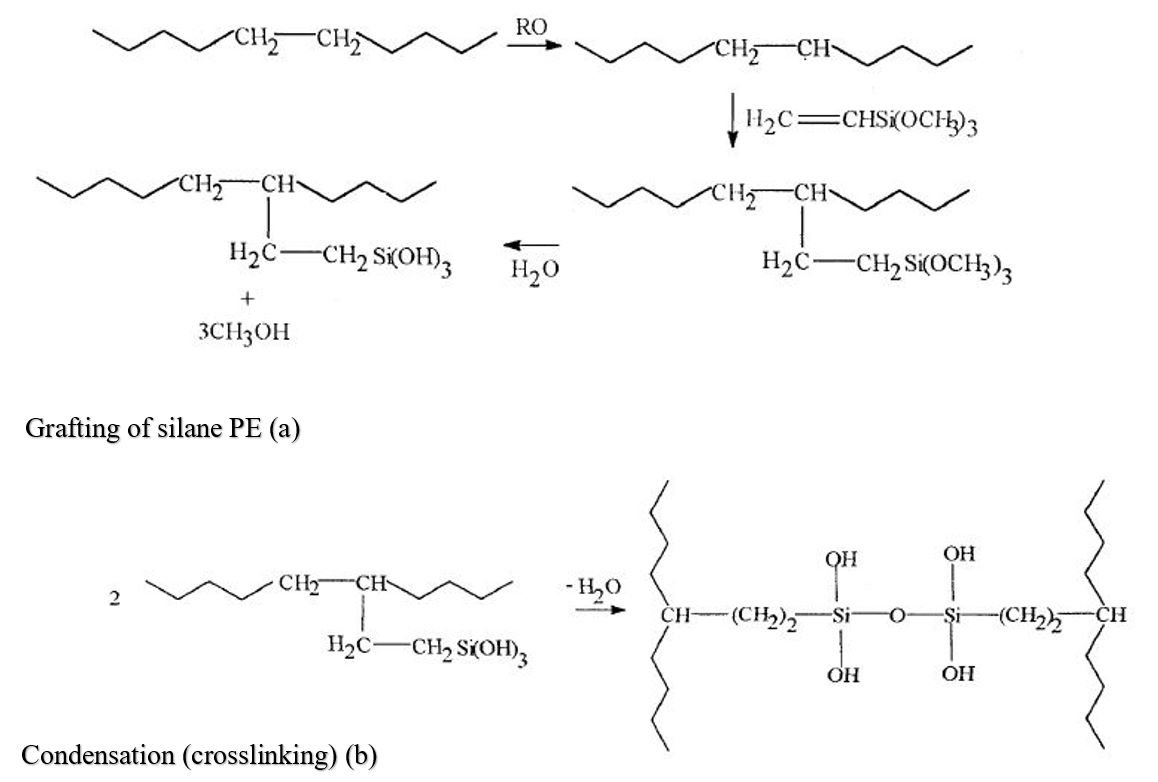
\includegraphics[width=\textwidth]{new_fig_2.jpg}
\caption{Silane grafted polyethylene crosslinking reaction (\cite{kurtz2009cross}).}
\label{ch3:figure:reaction}
\end{figure}

\paragraph{Radiation (physical) processes} \hfill \\
In contrast to chemical processes, radiation processes do not necessarily require any addition of any sort of chemicals in the original compound of \acrshort{pe}. In the radiation method, crosslinking is significantly achieved by the free radical mechanism, which is generated in a radiation polymer chain using high energy (\cite{peacock2000handbook}). As a consequence, two or more chains will join together where the free radical is generated. Figure \ref{ch3:figure:radiation} shows a schematic process of crosslinking \acrshort{pe} by radiation.

\begin{figure}[H]
\captionsetup[subfigure]{justification=raggedright}
\centering
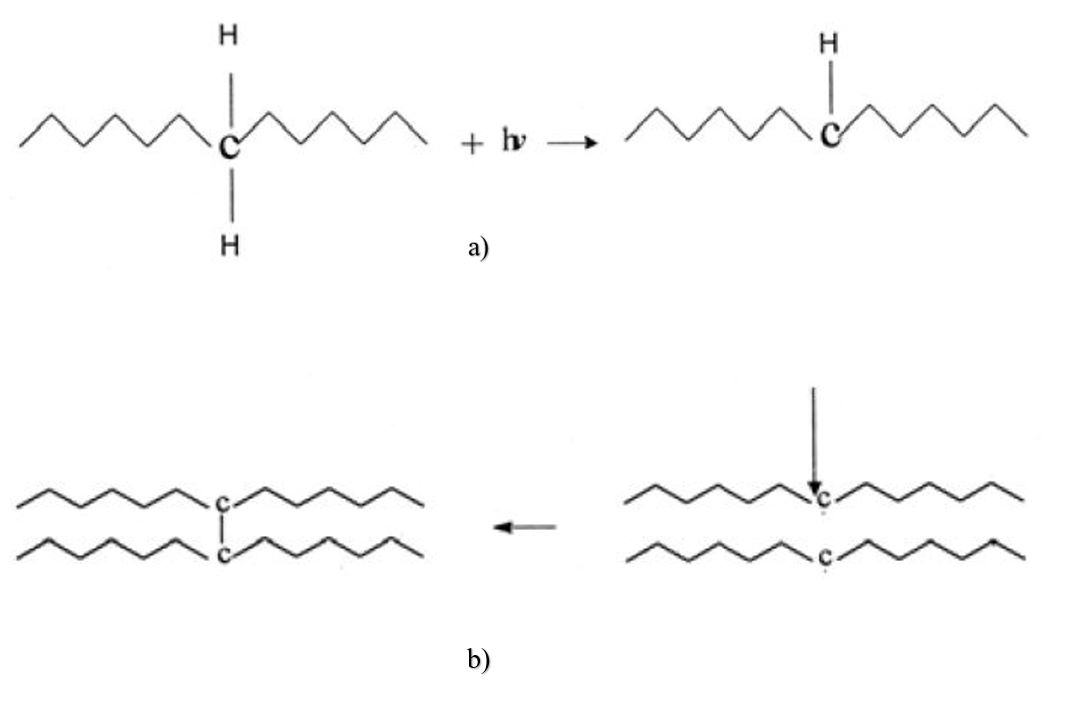
\includegraphics[width=\textwidth]{new_fig_1.jpg}
\caption{Polyethylene energy radiation (a) and the resulting crosslinked PE (b) (\cite{peacock2000handbook}).}
\label{ch3:figure:radiation}
\end{figure}

The involvement of high energy radiation on polymeric materials can critically produce crosslinking or cause a degradation in the main chain, which is termed ‘scission’ (\cite{meola2005cross}). In this way, both chain scission and crosslinking occur simultaneously and competitively. However, the dominance of one or the other may significantly depend upon several factors such as the sensitivity of the polymer to radiation, irradiation dose, and polymer radiation environment (\cite{meola2005cross}). To be precise, in the presence of oxygen (O2) scission is relatively dominant over crosslinking, while in an environment that contains other gases such as nitrogen (Ni), crosslinking is normally dominant (\cite{peacock2000handbook}). However, the changes and chemical properties of the finished product depend mostly on the efficiency of the crosslinking reaction and its relative ratio with degradation (\cite{meola2005cross}). For \acrshort{afff} storage facilities chemical properties of the cross-linked polymer are of great importance. This is due to the uses of \acrshort{afff}, as its chemical composition should not be influenced by the holding storage facility.

Mathematically, the scission and crosslinking can be related in order to estimate the probability between them. This probability can be expressed as a ratio that is given by the following equation.

\begin{equation}
    \frac{\beta}{\alpha}=\frac{1}{2}\frac{G(S)}{G(X)}
\end{equation}

\begin{doublespace}
\noindent Where, \\
$\alpha\ is\ a\ probability\ of\ crosslinking\ of\ chains\ after\ one\ electron\ volt\ of\ energy\ absorbed.$ \\
$\beta\ is\ a\ probability\ of\ chain\ scission\ after\ one\ electron\ volt\ of\ energy\ absorded.$ \\
$G(X)\ is\ a\ number\ of\ crosslinking\ per\ 100eV\ of\ radiant\ energy\ absorbed.$ \\
$G(S)\ is\ a\ number\ of\ scission\ per 100eV\ of\ energy\ absorbed.$ \\
\end{doublespace}

The typical G(X) and G(S) values are listed in Table \ref{appendix:classifications} on appendices. \\

According to several scientists the bond energy for breaking of C-H bond is typically 364Kj/mol (\cite{peacock2000handbook}). Therefore, the electron beam having sufficient energy to break C-H bond is normally suitable for crosslinking rather than scission (\cite{peacock2000handbook}). The technique of crosslinking \acrshort{pe} by radiation normally involves the four main variables. 

\begin{itemize}
    \item The type of radiation and its sources.
    \item The nature of \acrshort{pe} structure to irradiated.
    \item Mechanism and theories of reaction.
    \item The properties of the network formation, especially physical, chemical, and mechanical. 
\end{itemize}

\subsection{Environmental Stress Crack Resistance (ESCR)}
\acrshort{afff} concentrate contains sensitive chemicals within its composition. Therefore, under certain temperature and stress conditions, the \acrshort{pe} material may begin to crack sooner than expected due to the presence of chemicals contained in the \acrshort{afff} concentrate. It has been experimentally proven that storage facilities containing chemically free liquids do not suffer from cracks as much as those containing chemical liquids. This phenomenon is known as the environmental stress crack (ESC). One of the objectives of the present work is to assess and evaluate the chemical resistance of \acrshort{hdpe} in the presence of \acrshort{afff} concentrate. The test methods that are usually utilised to evaluate ESC and other substances are provided in Figure \ref{appendix:classifications} in the appendices. 

All engineering materials that are suitable for storing liquids containing chemicals are critically evaluated against ECS. For \acrshort{pe}, normally the stress-cracking agents are polar materials such as alcohols, detergents, halogens and aromatics (\cite{gabriel1998history}). \acrshort{afff} may be thought of as a detergent due to the bubbles it creates during utilisation. Consequently, it causes problems for \acrshort{pe} polymers. The property of a material to resist ESC is called environmental stress crack resistance (ESCR) (\cite{gabriel1998history}). Researchers have been working on understanding the mechanism of ESCR, however, to date it is not entirely understood. In most instances, failures of \acrshort{pe} polymers that are caused by ESC tend to be due to the development of cracks in area tensile stress which gradually grow and propagate over time (\cite{peacock2000handbook}).

Over the past years, there have been several efforts made in order to avoid ESC. Therefore, using an appropriate resin formulations of ESCR materials, designing the geometric appropriately, carefully using the manufacturing controls that prevents occurrence of severe stress risers, and limiting stresses and strains during the storage facility installation, all these are usually sufficient to avoid ESC (\cite{gabriel1998history}). Moreover, \acrshort{pe} polymer may be cross-linked to improve the chemical properties and thus resist cracking.  With this regard, it is vital to test the compatibility of \acrshort{pe}, especially \acrshort{xlpe} with \acrshort{afff} concentrate in order to avoid unexpected circumstances during fire conditions. To date, there are over 40 different ESCR test methods that are used to determine the chemical resistance of various materials. The standard test that is currently used in the industry of polyethylene is bent-strip test (\cite{gabriel1998history}). The method is normally used to assess the performance of polyethylene cable insulation but can be cautiously used to evaluate the performance of \acrshort{xlpe} storage facilities in the presence of \acrshort{afff} concentrate. The bent-strip test is shown in Figure \ref{ch3:figure:bending_apparatus}. Where the specimen is immersed into a surfactant of interest, and the time to failure is noted. The results are reported using the notation $F_{xx}$, where xx is the percentage of samples that has been tested.
 
\begin{figure}[H]
    \centering
    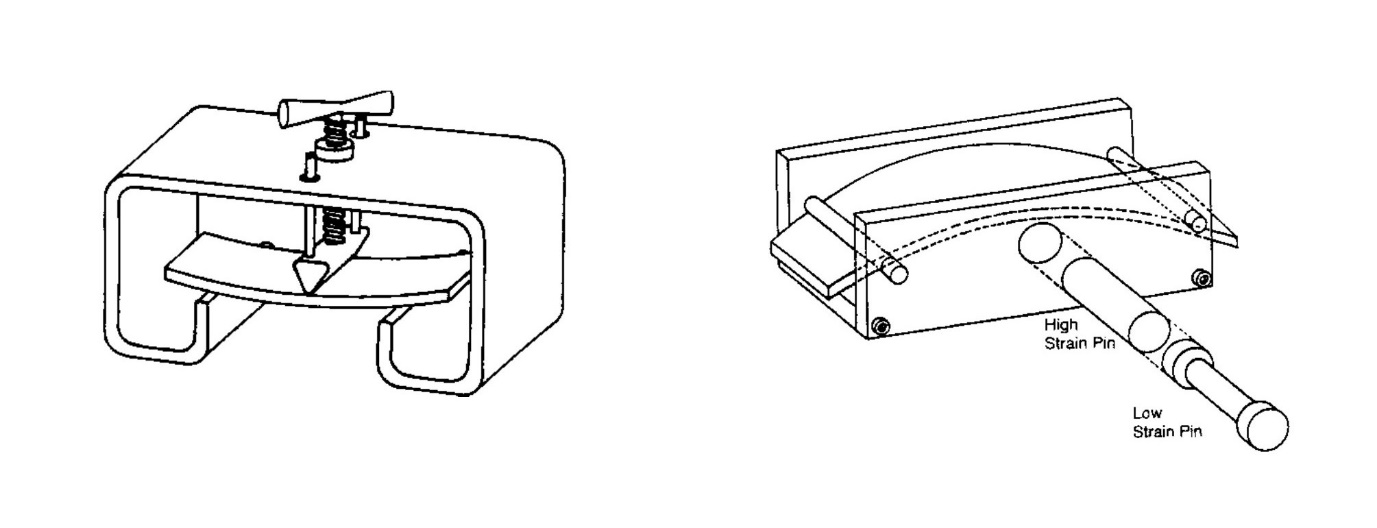
\includegraphics[width=.8\textwidth]{three_point_bending_apparatus_for_testing_escr.jpg}
    \caption{Three point bending apparatus for testing ESCR under constant strain (\cite{choi2009modeling}).}
    \label{ch3:figure:bending_apparatus}
\end{figure}

Research shows that the density of the \acrshort{pe} polymer plays a critical role towards ESCR. For \acrshort{pe} resins of the same molecular weight, the lesser the density, the greater the ESCR. The greater the proportion of crystals, the greater the density and the brittleness of the resin, which causes a rapid crack initiation (\cite{gabriel1998history}). However, since the phenomenon of ESC is not fully understood, then the density alone is inadequate to predict the ESCS.

\section{Conclusion}
This chapter discussed the engineering materials investigated in the present study. Both metals and plastics materials were closely assessed. The previous research was studied; this was used as a benchmark in this research. The atomic bonding, cross-linking methods, properties of interest, microstructure, and heat treatment processes are investigated. The properties of most materials depend upon the microstructure. Consequently, heat treatment processes are vital when improving these properties to better store \acrshort{afff} concentrate.

\acrshort{pe} plastics are rapidly replacing metals nowadays. They have several advantages over metal, as they are light in weight, resistant to corrosion, durable, and relatively affordable. These plastics are often classified by the density they possess. In this chapter, the environmental stress-cracking resistance of these plastics was discussed. To alter the properties of \acrshort{pe}, a cross-linking method was opted for. To date, this is an effective method to avoid the phenomenon of ESC.

The next chapter discusses and compares the various methods of constructing storage facilities for \acrshort{afff} concentrate. The methods used to test the compliance of these storage facilities are discussed. Both national and international design standards are considered.
\chapter{Experimental setup and methodology}
\label{ch4:anchor:chapter}

\section{Introduction}
In this chapter, the aim of the experiment, the experimental procedure, the materials, the analyses of samples, and the detailed experimental methods employed are all concisely described. Analyses of the methods and testing standards used are provided. All the parameters used are discussed and shown, and the safety precautions are followed throughout the experiments. After the \acrshort{afff} concentrate has been reacted with various engineering materials, the functional groups, particle shape and size, particle size distribution, and elemental composition are critically analyzed.

\section{Aim of the experiment}
The experimental work aims to evaluate and assess the impact and compatibility of the materials used to construct the storage facility with the \acrshort{afff} concentrate. The incompatibility of these materials can greatly influence the performance parameters of an \acrshort{afff} solution.  

\section{Methodology}
Samples of stainless steel, mild steel, and \acrshort{hdpe}, together with \acrshort{afff} concentrate, were carefully prepared. A guillotine machine was used to cut the material sheets into the desired shapes and sizes. All the material sheets were cut to the same sizes and shapes for a fair comparison. A total of three samples were used during the experiments. These sample materials were exposed to natural environmental conditions for 3 months. All the samples were then immersed and soaked in a 3\% proportion of \acrshort{afff} concentrate for 5 months. \Acrfull{ftir}, \acrfull{tem}, \acrfull{dls}, and \acrfull{icp} wet analysis were performed on samples of \acrshort{afff} concentrate. This was done to analyze any critical changes in the parameters of \acrshort{afff} concentrate after being in reaction with these materials. All the findings were carefully recorded and analyzed. However, it should be noted that the objective was to analyze the \acrshort{afff} concentrate, not the engineering materials. The experimental procedure followed for all the samples is presented in the flowchart in Figure \ref{ch4:figure:procedure}. 

\begin{figure}[H]
\centering

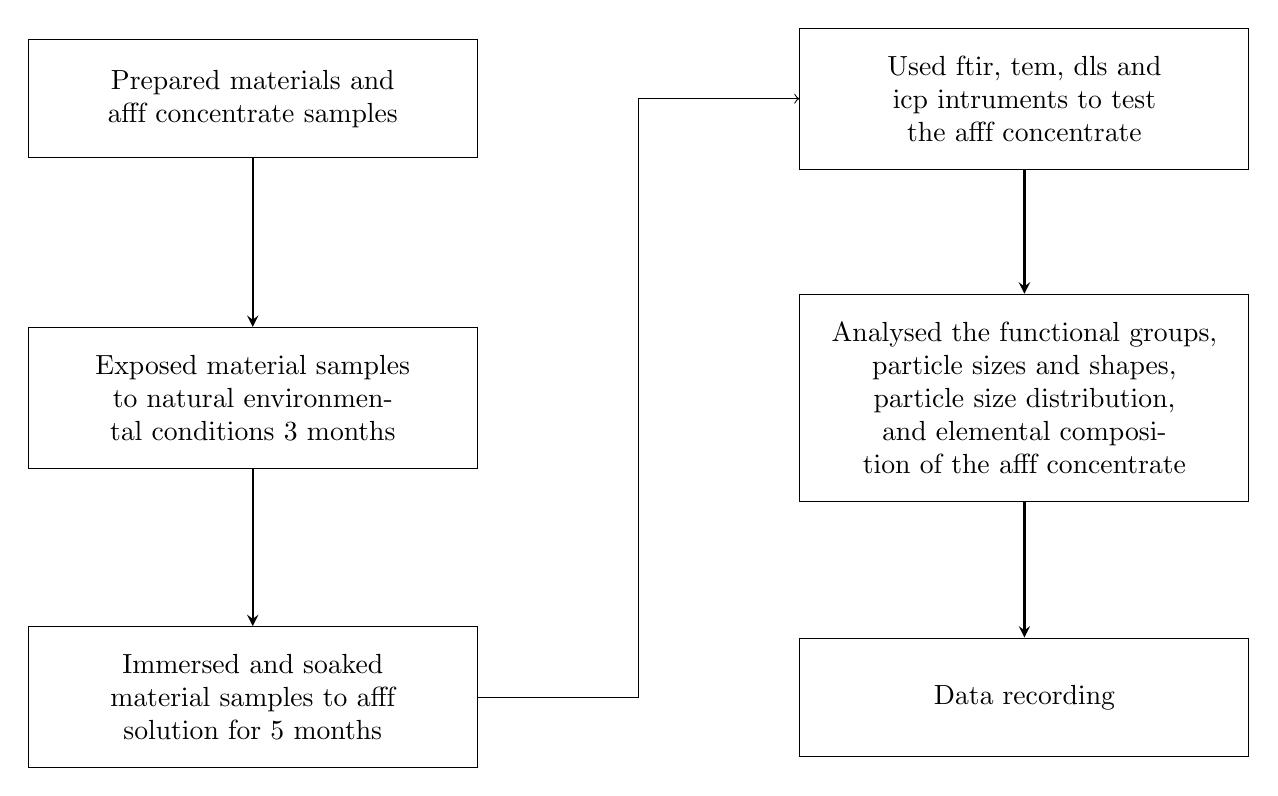
\begin{tikzpicture}[node distance=3.8cm]
    \tikzstyle{block} = [rectangle, minimum height=1.5cm, inner sep=1em, text centered, text width=5cm, draw=black]
    \tikzstyle{arrow} = [thick, ->, >=stealth]

    \node (prepare) [block] {Prepared materials and \acrshort{afff} concentrate samples};

    \node (expose) [block, below of=prepare] {Exposed material samples to natural environmental conditions 3 months};

    \node (immerse) [block, below of=expose] {Immersed and soaked material samples to \acrshort{afff} solution for 5 months};

    \node (use) [block, right of=prepare, xshift=6cm] {Used \acrshort{ftir}, \acrshort{tem}, \acrshort{dls} and \acrshort{icp} intruments to test the \acrshort{afff} concentrate};

    \node (analyse) [block, below of=use] {Analysed the functional groups, particle sizes and shapes, particle size distribution, and elemental composition of the \acrshort{afff} concentrate};

    \node (record) [block, below of=analyse] {Data recording};

    \newcommand*{\connector}[4][]{
        \draw[#1] (#3) -| ($(#3) !#2! (#4)$) |- (#4);
    }

    \draw [arrow] (prepare) -- (expose);
    \draw [arrow] (expose) -- (immerse);

    \connector[->, black]{0.5}{immerse}{use}

    \draw [arrow] (use) -- (analyse);
    \draw [arrow] (analyse) -- (record);

\end{tikzpicture}

\caption{Typical experimental procedure}
\label{ch4:figure:procedure}
\end{figure}

\section{Sample preparation}
\subsection{Material plates}
The 3, 4, and 5 mm thick sheets of mild steel, The 3, 4, and 5 mm thick sheets of mild steel, stainless steel, and \acrshort{hdpe}, respectively, were prepared for the experiments. The stainless steel was provided specially by Columbus Stainless (Pty) Ltd. The sizes are based on the common thickness of the storage tanks that contain the \acrshort{afff} concentrate, as investigated by \cite{protopopoff2011surface}.

These sheets were required to be cut to the desired shapes and sizes so that they could fit in 800 ml beakers filled with \acrshort{afff} concentrate. The scriber was used to scribe the precise sizes and shapes to be cut. This was done at the Durban University of Technology (DUT) manufacturing workshop using a guillotine-cutting machine. The prepared material samples can be seen in Figure \ref{ch4:figure:samples} (a-c).

\begin{figure}[H]
    \centering
    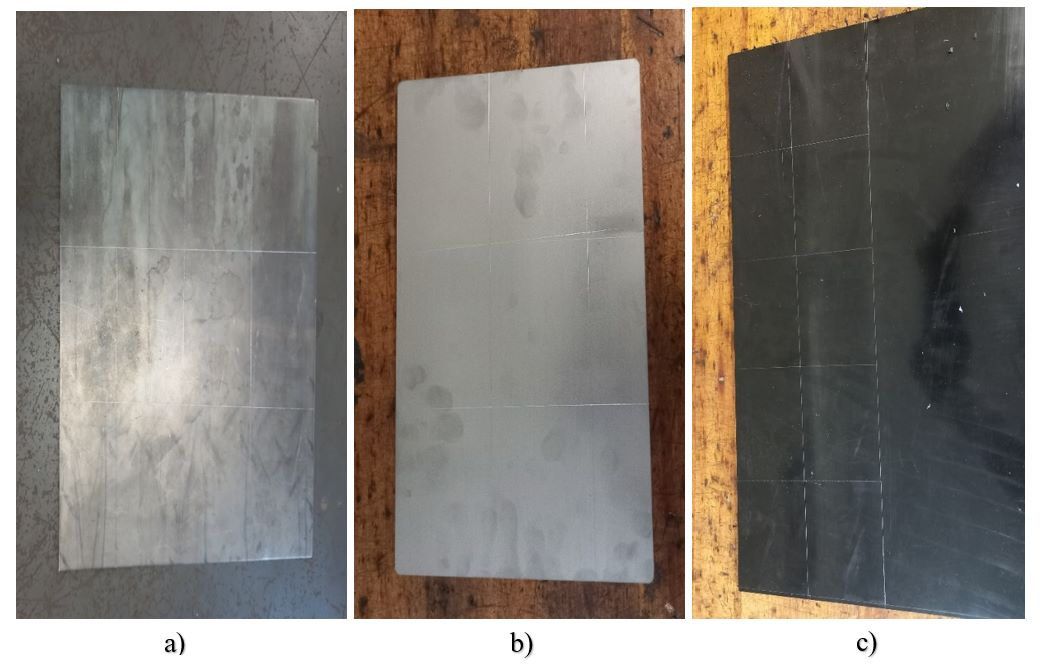
\includegraphics[width=\textwidth]{new_fig_3.jpg}
    \caption{Mild steel (a), stainless steel (b), and HDPE (c).}
    \label{ch4:figure:samples}
\end{figure}

\subsection{The cutting process}
The prepared samples were cut to sizes 60 mm by 100 mm using a guillotine machine. It can be seen in Figure \ref{ch4:figure:samples} (a-c) that the samples were first scribed before being cut to ensure precision. Mild steel and stainless steel were cut using a guillotine that can cut up to a thickness of 5 mm. In contrast, \acrshort{hdpe} was cut with a guillotine that can cut up to 3 mm of thickness, as it is not as hard as the two sheets of steel. Figure \ref{ch4:figure:guillotines} (a-b) shows the two guillotine machines that were used to cut the samples.

\begin{figure}[H]
    \centering
    \includegraphics[width=\textwidth]{3mm_and_5mm_guillotine_machine.jpg}
    \caption{Guillotine machines that cuts up to 5 (a) and 3mm (b) thickness, respectively.}
    \label{ch4:figure:guillotines}
\end{figure}

As aforementioned, the samples were cut into numerous pieces in the desired shapes and sizes to fit in the 800 ml glass beakers. Figure \ref{ch4:figure:samples_cut} shows the samples after the cutting process.

\begin{figure}[H]
    \centering
    \includegraphics[width=\textwidth]{samples_after_being_cut.jpg}
    \caption{Samples after being cut to the desired sizes, mild steel, stainless steel, and HDPE (left to right).}
    \label{ch4:figure:samples_cut}
\end{figure}

The samples were polished and cleaned using the rectangular file. This was done to remove the roughness and dangerous chips, to avoid any possible injuries during the experimental setup. Figure \ref{ch4:figure:file_and_vice} shows the tools used when cleaning and polishing the samples.
 
\begin{figure}[H]
    \centering
    \includegraphics[width=.6\textwidth]{rectangular_file_and_bench_vice.jpg}
    \caption{Rectangular file and bench vice}
    \label{ch4:figure:file_and_vice}
\end{figure}

\subsection{AFFF concentrate samples}
The 3\% \acrshort{afff} concentrate samples were prepared in 20-liter batches and kept at room temperature in the DUT laboratory. These were carefully stored in their original containers until the material sheet samples were available and ready. Figure \ref{ch4:figure:suplier} shows the \acrshort{afff} concentrate from the supplier in its original 20-liter container.
 
\begin{figure}[H]
    \centering
    \includegraphics[width=.5\textwidth]{pure_afff_concentrate_from_supplier.jpg}
    \caption{Pure \acrshort{afff} concentrate from the supplier.}
    \label{ch4:figure:suplier}
\end{figure}

To immerse various material samples, \acrshort{afff} concentrate was filled in respective glass beakers. Figure \ref{ch4:figure:immersed} shows the three glass beakers used to immerse the three materials of interest.
 
\begin{figure}[H]
\includegraphics{mild_stainless_steel_and_hdpe_immersed_in_afff_concentrate.png}
\caption{Mild steel, stainless steel, and HDPE (left to right) samples immersed in AFFF}
\label{ch4:figure:immersed}
\end{figure}

\subsection{Experimental matrix}

\begin{table}[H]
\centering
\caption{Experimental matrix with \acrshort{afff} concentrate.}

\renewcommand{\arraystretch}{2.5}
\begin{tabularx}{\textwidth}{ XXX }
    \hline
    Material & Instrument & Analyses \\
    \hline
    \acrshort{afff} concentrate & \acrshort{ftir} & Functional groups \\
    & \acrshort{tem} & Particle size and shape \\
    & & HR imaging \\
    & & Electron diffraction images \\
    & \acrshort{dls} & Particle size \\
    & & Particle size distribution \\
    & \acrshort{icp} & Elementary identification \\
    \hline
\end{tabularx}

\end{table}

\section{Testing} 
The different tests that were performed after the experiments are discussed in this section. The apparatus and various materials used to conduct the tests are concisely described.

\subsection{Fourier transform infrared spectroscopy (FTIR)}
All the \acrshort{afff} concentrate samples were analyzed using the \acrshort{ftir} technique. This was accomplished by comparing the manufacturer's pure \acrshort{afff} concentration to others that had reacted with the materials of interest. The \acrshort{ftir} analysis assisted in identifying the functional groups for various exposed samples, and the instrument can be seen in Figure \ref{ch4:figure:ftir}.
 
\begin{figure}[H]
    \centering
    \includegraphics[width=.75\textwidth]{ftir_instrument.jpg}
    \caption{FTIR instrument used to identify the functional groups.}
    \label{ch4:figure:ftir}
\end{figure}

\subsection{Transmission electron microscopy (TEM)}
Since the \acrshort{ftir} does not provide conclusive information, it was essential to validate the \acrshort{ftir} analysis with other tests. \acrshort{tem} analyses were conducted to analyze the overall particle shape and the visual overall size of the \acrshort{afff} concentrate particles using HR imaging and electron diffraction images. It should be noted that \acrshort{tem} does not provide sufficient information on how the particles in the exposed \acrshort{afff} concentrate are distributed and does not convey precise particle sizes. Consequently, the other relevant tests were necessary. The \acrshort{tem} instrument used for the tests is depicted in Figure \ref{ch4:figure:tem}.
 
\begin{figure}[H]
    \centering
    \includegraphics[width=.75\textwidth]{tem_instrument.png}
    \caption{TEM instrument used to analyze AFFF concentrate particles.}
    \label{ch4:figure:tem}
\end{figure}

\subsection{Dynamic Light Scattering (DLS)}
The \acrshort{dls} tests were conducted to deduce the particle size distribution and precise particle sizes using the instruments shown in Figure \ref{ch4:figure:dls}. This was achieved by measuring the hydrodynamic diameter (Z-average) of any present particles in units of nm. This was done to validate the findings of \acrshort{tem}, and it furthered an in-depth understanding of the behaviour of the \acrshort{afff} concentrate particles when exposed to various materials and how these materials affect their performance parameters.
 
\begin{figure}[H]
    \centering
    \includegraphics[width=.75\textwidth]{dls_instrument.png}
    \caption{DLS instrument used to analyze particle distribution of AFFF concentrate.}
    \label{ch4:figure:dls}
\end{figure}

\subsection{Inductively Coupled Plasma Atomic Emission Spectroscopy (ICP-AES)}
Finally, \acrshort{icp-aes} tests were performed to determine the elemental composition of the exposed \acrshort{afff} concentrate and compare it to the standard qualities. The changes in elemental composition can greatly affect the properties, hence the performance of \acrshort{afff} during firefighting circumstances. Thus, it is vital to assess the impact of the various materials on the composition of the \acrshort{afff} concentrate. Figure \ref{ch4:figure:icp-aes} shows the \acrshort{icp-aes} instrument used during the tests.
 
\begin{figure}[H]
    \centering
    \includegraphics[width=.75\textwidth]{icp_instrument.png}
    \caption{ICP-AES instrument used for elementary analysis.}
    \label{ch4:figure:icp-aes}
\end{figure}

\section{Conclusion}
The present chapter outlined the aim of the experiment, the material description, sample preparation, the techniques employed to test the samples and as well as the equipment and testing standards used. The instruments used for analyzing the \acrshort{afff} concentrate samples were presented with a thorough explanation of the purpose of each test. The experimental procedure followed in this investigation was explained. The results of the investigation are presented in Chapter \ref{ch5:anchor:chapter}.
\chapter{Results and discussions}
\label{ch5:anchor:chapter}
\section{Introduction}
In this chapter, the results of the experimental tests conducted during this study are concisely presented and discussed. The variation and correlation observed are also presented. This chapter builds from the experimental method (Chapter \ref{ch4:anchor:chapter}).  Four tests were conducted as shown in the previous chapter, this was done to validate the objectives of the present study, which is to investigate the effect of mild steel, stainless steel, and \acrshort{hdpe} on \acrshort{afff} concentrate. 

To begin with, the \acrshort{ftir} results were analyzed to deduce the functional groups of the \acrshort{afff} concentrate. The \acrshort{tem} was used to determine the overall size and shape of the particles; the \acrshort{dls} was used to determine the particle size distribution; and lastly, the \acrshort{icp-aes} was used to identify the elemental composition within the \acrshort{afff} concentrate.

\section{AFFF concentrate infrared spectroscopy}
Figure \ref{ch5:figure:spectra} shows the \acrshort{ftir} spectra of the pure \acrshort{afff} concentrate compared to the \acrshort{afff} concentrate that has been exposed to the materials of interest. Their functionality in terms of stability, oxidation, and reactivity was revealed. Unsurprisingly, most of the chemical and functional groups appear within the group frequency of 4000–1500 cm$^{-1}$ wavenumber 4000-1500 cm$^{-1}$.

Referring to \ref{ch5:figure:spectra} (a), it can be observed that at the single bond region, broadband appears at 3355 cm$^{-1}$, which has been associated with a hydroxy group, the H-bonded OH stretch (\cite{krimm1986vibrational}). This functional group is responsible for enhancing the ability of the \acrshort{afff} concentrate surfactants to dissolve in water (\cite{coates1996interpretation}).  Medial alkyne C$\equiv$C stretch appears as a weak band at 2120 cm$^{-1}$; this is a vital distinguishing tool since very few organic compounds reveal an absorption in this region (\cite{bellamy1980infrared}). The medium band detected at 1637 cm$^{-1}$ can be assigned to alkenyl C=C stretch vibration. Interestingly, the fingerprint region also revealed quite a few functional groups. However, the methylene C-H bend and skeletal C-C vibrations can be disregarded since they appear in most organic compounds. Furthermore, the fluoro-compound C-F stretch at 1083 cm$^{-1}$ confirms the presence of fluorosurfactant in \acrshort{afff} concentrate. This C-F compound slightly shifted when the materials were immersed in \acrshort{afff} concentrate, with the largest shift observed when mild steel was immersed.

Referring to Figure \ref{ch5:figure:spectra} (b), which compares the \acrshort{ftir} spectra of pure \acrshort{afff} concentrate with \acrshort{afff} concentrate that has been exposed to materials of interest to deduce the significant shifts of functional groups in the single-bond region, a hydroxy group, H-bonded OH stretch, still appears in all the \acrshort{ftir} spectra. However, there is a strange absorption peak of aldehyde C-C stretching that appears in \acrshort{afff} concentrate after \acrshort{hdpe} and stainless steel were immersed at bands 2710 and 2697 cm$^{-1}$, respectively (\cite{lin1991handbook}). This may indicate an interaction between the \acrshort{afff} concentrate and these two materials. Moreover, there is a significant shift that can be observed in the triple bond region at bands 2056 and 2060 cm$^{-1}$ for exposed \acrshort{hdpe} and stainless steel \acrshort{afff} concentrate, respectively. Consequently, this shift confirms the presence of isothiocyanate N=C=S stretching, which is a very unusual functional group, especially in organic compounds

It can be clearly observed that there are minor shifts in the functional groups. However, these minor shifts can be subsequently used to predict the reaction of the materials with the \acrshort{afff} concentrate in the long term. This is a very useful prediction technique since, in the present study, these materials were immersed in \acrshort{afff} concentrate for only five months. Furthermore, the major reaction in the real world could take years. Figure \ref{ch5:figure:materials} (a-c) in Section \ref{ch5:anchor:section:spectroscopy} compares the \acrshort{ftir} spectra of the pure mild steel, stainless steel, and \acrshort{hdpe} to others that have been immersed in \acrshort{afff} concentrate. This was done to further examine and validate the functional group shifts on the exposed materials of interest.

\begin{figure}[H]
\centering

\begin{subfigure}{.45\textwidth}
    \includegraphics[width=\textwidth]{ftir_spectra.png}
    \caption{}
    \label{ch5:figure:spectra:a}
\end{subfigure}
\begin{subfigure}{.45\textwidth}
    \includegraphics[width=\textwidth]{comparison.png}
    \caption{}
    \label{ch5:figure:spectra:b}
\end{subfigure}

\caption{Comparisons Pure AFFF spectra (a) with the other materials after they were immersed (b).}
\label{ch5:figure:spectra}
\end{figure}

\section{Infrared spectroscopy of HDPE, Mild steel, and Stainless steel}  
\label{ch5:anchor:section:spectroscopy}

The \acrshort{ftir} spectra of the materials of interest were conducted to substantiate the minor shifts of the functional group on the exposed \acrshort{afff} concentrate. Figure \ref{ch5:figure:materials} (a-c) shows the \acrshort{ftir} spectra of the materials of interest. The reactivity of \acrshort{afff} concentrate with the materials was of particular interest. It can be observed from Figure \ref{ch5:figure:materials} (a-c) that there are significant shifts in functional groups. In Figure \ref{ch5:figure:materials} (a), the O-H stretching, which can be observed at 3583 cm$^{-1}$ in pure \acrshort{hdpe}, shifted to a wavenumber of 3817 cm$^{-1}$ when the materials were immersed in \acrshort{afff} concentrate (\cite{mudunkotuwa2014atr}). In pure \acrshort{hdpe}, a strong amine N-H stretching at 3358 cm$^{-1}$ can be seen, which shifts to a broad band at 3406 cm$^{-1}$ in immersed concentrate (\cite{mohamed2017fourier}).

\begin{figure}[H]
\centering

\begin{subfigure}{.45\textwidth}
    \includegraphics[height=6cm, width=\textwidth]{pure_hdpe_ftir_spectra.png}
    \caption{}
\end{subfigure}
\begin{subfigure}{.45\textwidth}
    \includegraphics[height=6cm, width=\textwidth]{pure_ms_ftir_spetra.png}
    \caption{}
\end{subfigure}
\begin{subfigure}{.45\textwidth}
    \includegraphics[width=\textwidth]{pure_ss_ftir_spectra.png}
    \caption{}
\end{subfigure}

\caption{FTIR spectra, comparing various materials.}
\label{ch5:figure:materials}
\end{figure}

\section{Transmission electron microscopy (TEM)}
The JEOL JEM-1010 \acrshort{tem} used for the present study is equipped with highly integrated technology. The 40 kV to 100 kV operating voltage range is suitable for applications in material science. Because of its low operating voltage and unique objective pole piece design, the JEM-1010 is a \acrshort{tem} with outstanding contrast (\cite{klein2011transmission}). Additionally, it has a 2K x 2K AMT CCD camera for taking digital images. Using high resolution (HR) and electron diffraction imaging, the \acrshort{tem} was able to provide overall particle shape, a large variety of particles, and a visual overall of the particle shape of the \acrshort{afff} concentrate samples. 

The \acrshort{tem} images of pure \acrshort{afff} concentrate are shown in Figure \ref{ch5:figure:pure_afff_images}. These are utilized as a benchmark and compared to the immersed concentrate to observe any critical particle changes. All the samples depict the HR and electron diffraction images in various parts. This was done to understand the overall particle shape of the concentrate before making any conclusions.

\begin{figure}[H]
\centering
\includegraphics[width=.88\textwidth]{new_fig_4.jpg}

\caption{HR (a-c) and electron diffraction images (d) of pure AFFF concentrate.}
\label{ch5:figure:pure_afff_images}
\end{figure}

It can be observed from Figure \ref{ch5:figure:pure_afff_images} (d) that the electron diffraction image of pure \acrshort{afff} concentrate provides numerous spots that are aligned in a particular direction. This is a demonstration that the concentrate in a pure state has a single crystalline structure. This shows that the concentrate has uniform properties and is more stable in its pure form (\cite{bandyopadhyay2019fabrication}). Moreover, Figure \ref{ch5:figure:pure_afff_images} (a-c) reveals that the particles of pure \acrshort{afff} concentrate are scattered along the concentrate. This might be caused by the collision of two or more repelling particles within the concentrate (\cite{pyrz2008particle}). Figures \ref{ch5:figure:mild_steel_images} - \ref{ch5:figure:hdpe_images} depict the HR and electron diffraction images when various materials were immersed in \acrshort{afff} concentrate. 
  
\begin{figure}[H]
\centering

\includegraphics[width=.9\textwidth]{electron_diffraction_images_of_pure_AFFF_concentrate_4-8.png}

\caption{HR (a-c) and electron diffraction images (d) of AFFF concentrate immersed in mild steel.}
\label{ch5:figure:mild_steel_images}
\end{figure}

\begin{figure}[H]
\centering

\includegraphics[width=.9\textwidth]{electron_diffraction_images_of_pure_AFFF_concentrate_8-12.png}

\caption{HR (a-c) and electron diffraction images (d) of AFFF concentrate immersed in stainless steel.}
\label{ch5:figure:stainless_steel_images}
\end{figure}

\begin{figure}[H]
\centering

\includegraphics[width=.9\textwidth]{electron_diffraction_images_of_pure_AFFF_concentrate_12-16.png}

\caption{HR (a-c) and electron diffraction images (d) of AFFF concentrate immersed in HDPE.}
\label{ch5:figure:hdpe_images}
\end{figure}

The overall crystal structure and the difference in particle shape for the three samples compared to a pure \acrshort{afff} sample were studied. Although the present \acrshort{tem} analyses are not able to provide the precise particle sizes of the samples, they nonetheless provide a significant overall change in the crystal structure. Figure \ref{ch5:figure:pure_afff_images} revealed that in a pure state, \acrshort{afff} concentrate posses revealed that in a pure state, \acrshort{afff} concentrate possesses a single crystalline structure. However, when studying Figures \ref{ch5:figure:mild_steel_images} - \ref{ch5:figure:hdpe_images}, it is observed that the exposed \acrshort{afff} concentrate has critically changed to a polycrystalline structure. When closely inspecting the electron diffraction images of these samples, this is seen in Figures \ref{ch5:figure:mild_steel_images} - \ref{ch5:figure:hdpe_images} (d). The concentrated circular rounds imply that all these materials are polycrystalline. This is confirmed by the morphology (particles, grains, and crystallites), as several grains are observed in Figures \ref{ch5:figure:mild_steel_images} - \ref{ch5:figure:hdpe_images}. These grains are separated by grain boundaries and have random crystallographic orientations. It can be further observed that Figure \ref{ch5:figure:mild_steel_images} has more grains compared to Figures \ref{ch5:figure:stainless_steel_images} and \ref{ch5:figure:hdpe_images}. Consequently, this implies that most of the crystal structural changes occurred when mild steel was immersed in \acrshort{afff} concentrate.

When comparing the differences topographically (structure and shape), it can be observed in Figure \ref{ch5:figure:pure_afff_images} that the particles for pure \acrshort{afff} concentrate are scattered and distributed along the concentrate. However, when closely observing Figures \ref{ch5:figure:mild_steel_images} - \ref{ch5:figure:hdpe_images}, it can be seen that the particles for these samples are concentrated in one area, especially in Figure \ref{ch5:figure:mild_steel_images}. As a result, this demonstrates that when the materials of interest were immersed in \acrshort{afff} concentrate, there was a structural and shape particle change. The alteration in crystal structure and particle shape in \acrshort{afff} concentrate complements the shifts in functional groups obtained using \acrshort{ftir}. \cite{an2018effect} experimentally investigated the effect of the particle shape on the viscosity of the liquid. Their results indicated that the spherical particles have a lower viscosity, and any other particle shape will result in a higher viscosity. In addition, a change in any additives in \acrshort{afff} concentrate will affect the foam drainage time. It should be noted that the causes of these alterations are not known as of yet. However, conclusive results and interpretations are detailed in Sections \ref{ch5:anchor:section:dls} and \ref{ch5:anchor:section:analysis} using the \acrshort{dls} and elementary analysis to validate the vital information provided by \acrshort{ftir} and \acrshort{tem}.

\section{Dynamic light scattering (DLS)}
\label{ch5:anchor:section:dls}
In this section, an in-depth understanding of the cause of crystal structure and particle shape changes within the \acrshort{afff} concentrate and the impact these changes possess on the performance parameters are discussed. This is achieved by evaluating the particle size and particle size distribution of \acrshort{afff} concentrate by measuring the hydrodynamic diameter (Z-average) of any present particles in units of nanometers (nm) using a \acrshort{dls} technique. \acrshort{dls} is a noninvasive technique that depends on the particles moving randomly as a result of collisions with the solvent molecules (Brownian motion). As a result, only particles suspended in a liquid may be categorized (\cite{machhi2021effect}). The determination of particle size and size distribution is essential because these characteristics have a large effect on the properties of the \acrshort{afff} concentrate, including its mechanical stability, foaming ability, and a viscosity (\cite{de2017detection}).

\subsection{Particle size analysis}
\label{ch5:anchor:section:size_analysis}

Figure \ref{ch5:figure:samples} depicts the four samples used during the \acrshort{dls} analysis, where 1, 2, and 3 are \acrshort{afff} concentrates when mild steel, stainless steel, and \acrshort{hdpe}, respectively, have been immersed. Sample 4 is a pure \acrshort{afff} concentrate for benchmark purposes. Table \ref{ch5:table:sizes} shows the summary of the results for average particle sizes for the four samples in nm.
  
\begin{figure}[H]
    \centering
    \includegraphics[width=.7\textwidth]{samples_used_during_the_dls_analysis.png}
    \caption{Samples used during the DLS analysis.}
    \label{ch5:figure:samples}
\end{figure}

\begin{table}[H]
\renewcommand{\arraystretch}{2}

\caption{Summary of average particle sizes.}

\begin{tabularx}{\textwidth}{ XX }
\hline
\textbf{SAMPLE ID} & \textbf{Z-AVERAGE (D)} \\
\hline
\textbf{1} & 660.7 nm \\
\textbf{2} & 4.892 nm \\
\textbf{3} & 4.036 nm \\
\textbf{4} & 3.586 nm \\
\hline
\end{tabularx}

\label{ch5:table:sizes}
\end{table}

It can be observed from Table \ref{ch5:table:sizes} that there have been changes in particle diameter. The pure \acrshort{afff} concentrate has an average particle size of 3.586 nm, which is a very small particle size. However, when comparing this to samples 2 and 3, it can be observed that there is a slight difference or change. To be precise, the change in Z-average is around 1.306 nm at most. At this point, it is not known if these changes are slight enough to not affect the properties of \acrshort{afff} concentrate. Sample 1, in Table \ref{ch5:table:sizes}, shows a major change in particle size. Sample 1 has an average particle size of 660.7 nm, which is way above the other three samples by about 655.808 nm at most. This difference is extremely surprising and has some implications. \cite{koca2018effect} studied the effect of particle size on the properties of nanofluids. They discovered that larger particles have a slower diffusion speed than smaller ones. In a fluid, a particle's translational diffusion coefficient and hydrodynamic diameter are related by the Stokes-Einstein equation (\cite{an2018effect}), as demonstrated by Equation (\ref{ch5:equation:stokes_einstein}).

It can be observed from Table \ref{ch5:table:sizes} that there have been changes in particle size diameter. The pure \acrshort{afff} concentrate has an average particle size of 3.586 nm, which is a very small particle size. However, when comparing this to sample 2 and 3 it can be observed that there is a slight difference or change. To be precise, the change in Z-average is around 1.306 nm at most. At this point, it is not known if these changes are slight in such a way that they do not have any effect on the properties of \acrshort{afff} concentrate. Sample 1, in Table \ref{ch5:table:sizes} shows a major change in particle size. Samples 1 has an average particle size of 660.7 nm, which is way above the other three samples by about 655.808 nm at most. This difference is extremely surprising and obviously has some implications. As a matter of fact, larger particles have a gradual diffusion speed than smaller particles. In a fluid, a particle's translational diffusion coefficient and hydrodynamic diameter are related by the Stokes-Einstein equation (\cite{lin1991handbook}), as demonstrated by equation (\ref{ch5:equation:stokes_einstein}).

\begin{equation}
    D_T=\frac{K_bT}{b\pi \eta R_h}
    \label{ch5:equation:stokes_einstein}
\end{equation}

\begin{doublespace}
Where, \\
$D_T\ is\ the\ transitional\ diffusion\ coefficient\ in\ \nicefrac{m^2}{s}$ \\
$R_H\ is\ the\ hydrodynamic\ radius\ in\ m$ \\
$K_b\ is\ the\ Boltzmann\ constant\ in\ \nicefrac{J}{K}$ \\
$T\ is\ the\ Temperature\ in\ K$ \\
$\eta\ is\ the\ viscosity\ of\ the\ medium\ in\ \nicefrac{Ns}{m^2}$ \\
$b\ is\ the\ constant\ that\ depends\ on\ the\ size\ of\ the\ diffusing\ molecules$ \\
\end{doublespace}

As a matter of fact, for \acrshort{afff} stability, rapid diffusion of fluorosurfactant molecules is required. It can be observed from Equation (\ref{ch5:equation:stokes_einstein}) that the rate of diffusion is inversely proportional to the particle size. However, it also depends on the surface area and temperature. For the present study, all the samples were exposed to the same temperature (atmospheric) for an equitable comparison. This is a demonstration that once \acrshort{afff} concentrate has been in contact with mild steel, it decreases its diffusion rate rapidly and thus decreases the foaming stability of \acrshort{afff}.  On the other hand, the Z-average (particle size diameter) results demonstrate that when stainless steel and \acrshort{hdpe} have been immersed in \acrshort{afff} concentrate, there are slight differences in particle diameter when compared to pure \acrshort{afff} concentrate. When visually observing the numbers, the difference looks slight. On the contrary, the percentage increase calculations demonstrate a relatively large difference. The fundamental equation is given as:

\begin{doublespace}
\begin{eqnarray}
    \label{ch5:equation:stainless_steel}
    \%Increase &=& \frac{D_s - D_O}{3.586} \times 100 \\ 
    \nonumber &=& \frac{4.892 - 3.586}{3.586}\times 100 \\
    \nonumber &=& 36.419\%
\end{eqnarray}
\end{doublespace}

It is possible to calculate the percentage increase in particle size for the \acrshort{afff} concentrate when stainless steel was immersed.

\begin{doublespace}
Where, \\
$D_s\ is\ the\ particle\ size\ diameter\ of\ sample\ 2\ in\ nm$ \\
$D_O\ is\ the\ particle\ size\ diameter\ of\ sample\ 4\ in\ nm$ \\
\end{doublespace}

The same formula employed in Equation (\ref{ch5:equation:stainless_steel}) can be used to calculate the percentage increase in particle diameter for the \acrshort{afff} concentration when \acrshort{hdpe} was immersed. 

\begin{doublespace}
\begin{eqnarray}
    \label{ch5:equation:hdpe}
    \%Increase &=& \frac{D_s - D_O}{D_O} \times 100 \\ 
    \nonumber &=& \frac{4.036 - 3.586}{3.586}\times 100 \\
    \nonumber &=& 12.549\% 
\end{eqnarray}
\end{doublespace}
 
\begin{doublespace}
Where, \\
$D_s\ is\ the\ particle\ size\ diameter\ of\ sample\ 2\ in\ nm$ \\
$D_O\ is\ the\ particle\ size\ diameter\ of\ sample\ 4\ in\ nm$ \\
\end{doublespace}

It can be seen from Equation (\ref{ch5:equation:stainless_steel}) that the particle size percentage change is 36.419\% when stainless steel is immersed in \acrshort{afff} concentrate. This can be regarded as a huge increase since there is more than a quarter (1/4) difference between the two particles. When analyzing Equation (\ref{ch5:equation:hdpe}), it can be observed that when \acrshort{hdpe} was immersed in AFF concentrate, the particle size had an average change of 12.549 nm. This is a much smaller percentage compared to 36.419 nm, with a difference of 23.87 nm. However, it cannot be guaranteed that it does not affect the foaming ability of \acrshort{afff} concentrate. At this moment, there are still doubts regarding the effects of these materials on \acrshort{afff} concentrate. However, the analysis of the particle size distribution (PSD) and element composition will be conducted in Sections \ref{ch5:anchor:section:psd} and \ref{ch5:anchor:section:analysis}, respectively, for further validation.

\subsection{Particle size distribution (PSD) analysis}
\label{ch5:anchor:section:psd}
\acrshort{dls} is a widely accepted method to evaluate the hydrodynamic size of concentrate particles. The \acrshort{dls} particle size results can be represented using volume, number, and intensity. However, as stated in the international standard (\acrshort{iso} 22412:2017), intensity-based results are the most reliable parameters provided by \acrshort{dls} to describe particle size and particle size distribution (PSD) (\cite{ramirez2021characterization}). As a consequence, the intensity-based results were opted for in the present research work to analyze the PSD of pure \acrshort{afff} concentrate and \acrshort{afff} concentrate after the three materials were immersed. A comparison in size distribution is then made to understand the influence of each material on the properties of \acrshort{afff} concentrate. PSD is essential for understanding the chemical and physical properties of a sample. The particles within the \acrshort{afff} concentrate have similar sizes and are relatively uniform. The PSD curve of the pure \acrshort{afff} concentrate plotted by intensity is shown in Figure \ref{ch5:figure:pure_afff}. This PSD curve is used to compare the alteration in PSD of \acrshort{afff} concentrate when various materials were immersed.

\begin{figure}[H]
    \centering
    \includegraphics[width=\textwidth]{particle_size_distribution_of_pure_afff_solution.png}
    \caption{Particle size distribution of pure AFFF concentrate.}
    \label{ch5:figure:pure_afff}
\end{figure}

It can be observed from Figure \ref{ch5:figure:pure_afff} that the particle size distribution curve shows that the peaks are divided into three intensities. As expected, the major peak is at a particle size of 3.586 nm, as previously shown in Table \ref{ch5:table:sizes}, and the second and third peaks can be estimated at 350 and 5500 nm, respectively. \cite{de2017detection} studied the particle size distribution of aqueous concentrate. They demonstrated that the aqueous concentrate with a narrow PSD was able to disperse easily. Similarly, it can be seen from Figure \ref{ch5:figure:pure_afff} that the first peak is very narrow. As expected, this is evidence that in a pure state, \acrshort{afff} concentrate can disperse or spread rapidly over a large surface area.

\begin{figure}[H]
    \centering
    \includegraphics[width=.95\textwidth]{graph_5_9.jpg}
    \caption{Particle size distribution of AFFF concentrate when stainless steel was immersed.}
    \label{ch5:figure:stainless_steel}
\end{figure}

Referring to Figure \ref{ch5:figure:stainless_steel}, it is observed that the \acrshort{afff} concentrate possesses three peaks. This is precisely the same observation as in Figure \ref{ch5:figure:pure_afff}. Unsurprisingly, the main peak can be attributed to a particle size of 4.892 nm. Moreover, it can be seen from Figure \ref{ch5:figure:stainless_steel} that the main peak has a narrow PSD. However, when closely observed, it is slightly wider compared to Figure \ref{ch5:figure:pure_afff}. This demonstrates that stainless steel did not cause any critical alteration of PSD within the AFF concentrate, as it is still able to disperse easily. This is a validation that stainless steel does not influence the spreading ability of \acrshort{afff}. This further concludes that the minor particle size alteration discussed in Section \ref{ch5:anchor:section:size_analysis} and Equation (\ref{ch5:equation:stainless_steel}) does not have a significant impact on the diffusion rate of fluorosurfactant molecules.   
  
\begin{figure}[H]
    \centering
    \includegraphics[width=.95\textwidth]{graph_5_10.jpg}
    \caption{Particle size distribution of AFFF concentrate when HDPE was immersed.}
    \label{ch5:figure:hdpe}
\end{figure}

It can be observed from Figure \ref{ch5:figure:hdpe} that the PSD curve consists of peaks that are divided into two intensities. This is in contrast to Figures \ref{ch5:figure:pure_afff} and \ref{ch5:figure:stainless_steel}, where the peaks were divided into three intensities. The major peak can be associated with a particle size of 4.036 nm, whereas the other peak can be estimated at 5000 nm. When observing the broadness of the major peak, it can be noticed that it is wider than the peak in Figure \ref{ch5:figure:pure_afff} and almost the same size as Figure \ref{ch5:figure:stainless_steel}. This, however, can be considered a narrow peak. Moreover, this provides sufficient evidence that \acrshort{hdpe} does not alter the PSD within the pure \acrshort{afff} concentrate, which suggests that the dispersion rate is not affected. This further concludes that the minor particle size alteration discussed in Section \ref{ch5:anchor:section:analysis} and Equation (\ref{ch5:equation:hdpe}) does not have a significant impact on the diffusion rate of fluorosurfactant molecules.  
  
\begin{figure}[H]
    \centering
    \includegraphics[width=.95\textwidth]{graph_5_11.jpg}
    \caption{Particle size distribution of AFFF concentrate when mild steel was immersed.}
    \label{ch5:figure:mild_steel}
\end{figure}

Surprisingly, Figure \ref{ch5:figure:mild_steel} depicts a distinct PSD compared to Figures \ref{ch5:figure:pure_afff}-\ref{ch5:figure:hdpe}. It can be observed that Figure \ref{ch5:figure:mild_steel} reveals peaks that are divided into two intensities. These peaks can be associated with particle sizes of 660.7 nm, whereas the other peak can be estimated at 5500 nm. Due to the large difference in sizes between these two peaks, they can be generally regarded as major and minor peaks, respectively. It is interesting to note that Figure \ref{ch5:figure:mild_steel} possesses a wide major peak compared to all previous peaks illustrated in Figures \ref{ch5:figure:pure_afff}-\ref{ch5:figure:hdpe}. This is an indication that there has been a sensitive reaction between mild steel and \acrshort{afff} concentrate. Moreover, this demonstrates that the spreading ability of the concentrate has been reduced. This could be caused by several parameters, such as an increase in viscosity that causes the concentrate to be slightly thicker. However, it is well known that viscosity is largely dependent on the shape of the particles, where any deviation from the spherical shape of the particle increases viscosity (\cite{karau1997influence}). Nevertheless, it is noticed in Figure \ref{ch5:figure:mild_steel} that the alteration in PSD can have a slight impact on the spreading capability of the aqueous concentrate. 

\section{Wet chemical analysis}
\label{ch5:anchor:section:analysis}
As aforementioned, the \acrshort{icp-aes} was used to identify both the amounts and major concentrations of elements within the exposed \acrshort{afff} concentrate and benchmark these with the standard quantities and qualities. The alterations in elements or composition can immensely affect the properties, hence the performance of \acrshort{afff} during firefighting circumstances. The concrete results are provided in this section, and conclusive information is drawn regarding the severity of mild steel, stainless steel, and \acrshort{hdpe} on the performance parameters of \acrshort{afff}. In addition, the elementary results are more reliable as they provide the precise elements that are present within the \acrshort{afff} concentrate before and after the materials were immersed. Thus, they validate the previous results of the analyses conducted using \acrshort{ftir}, \acrshort{tem}, and \acrshort{dls}.

\subsection{Elemental componsition analysis}
For the present research, the elements were analyzed based on the importance of the role they possess within the \acrshort{afff} concentrate. To begin with, \acrshort{afff} is water-based and commonly contains a hydrocarbon-based surfactant such as sodium alkyl sulfate. They discovered that the presence of sodium and sulphur within these fluids is responsible for the stable foam formation. \cite{yu2020formation} studied the formation of stable aqueous foams. They experimentally demonstrated that the presence of sodium and sulphur within the aqueous solution is responsible for the stable foam formation. As a matter of fact, for stable foam formation, there must be less surface tension in the water. This is mostly accomplished by increasing the sodium alkyl sulfate concentration. As a consequence, sodium and sulphur were the primary elements of interest. Other elements were also analyzed at a later stage, and their impacts on the performance parameter of \acrshort{afff} were concisely discussed. Table \ref{ch5:table:chemical_elements_1} depicts the elemental composition results of the pure \acrshort{afff} concentrate and the other when mild steel, stainless steel, and \acrshort{hdpe} were immersed. The entire elemental composition results are depicted in Figures \ref{appendix:samples_1-3} and \ref{appendix:sample4} in the appendices for validation purposes.

\newcolumntype{Y}{>{\centering\arraybackslash}X}

\begin{table}[H]
\renewcommand{\arraystretch}{2}
\caption{Chemical elements of AFFF concentrate.}

\begin{tabularx}{\textwidth}{*{6}{Y}}
\hline
Element & Chemical symbol & \multicolumn{4}{c}{Composition in PPM} \\
& & \multicolumn{4}{c}{Sample ID:} \\
\hline
& & 1 & 2 & 3 & 4 \\
Sodium & Na & 2302 & 2332 & 2349 & 2354 \\
Sulphur & S & 92 & 89 & 94.2 & 94.7 \\
\hline
\end{tabularx}

\label{ch5:table:chemical_elements_1}
\end{table}

Referring to Table \ref{ch5:table:chemical_elements_1}, samples 1-3 are the \acrshort{afff} concentrate after mild steel, stainless steel, and \acrshort{hdpe} were immersed, respectively, with sample 4 being the pure \acrshort{afff} concentrate. From Table 4, it can be observed that in a pure state, \acrshort{afff} concentrate has 2354 and 94.7 parts per million (ppm) of sodium and sulphur, respectively. When observing closely, it is seen that the sodium in pure \acrshort{afff} concentrate (sample 4) decreases gradually. To be precise, the sodium is reduced by 5, 22, and 52 ppm, respectively, from the pure \acrshort{afff} concentrate. This indicates that the sodium composition of the \acrshort{afff} concentrate is reduced when it is exposed to the materials of interest. Moreover, it can be observed that the amount of reduction in sodium is diverse in all samples. This further demonstrates that the severity of the effects caused by the materials on the foam’s stability varies greatly.

Similar occurrences can be observed with sulphur. Referring to Table \ref{ch5:table:chemical_elements_1}, it is observed that the elemental composition of sulphur in pure \acrshort{afff} decreases when it reacts with various materials. Consequently, it is evident that the reaction of the three materials with the \acrshort{afff} concentrate reduces the surfactants (sodium alkyl sulfate). This increases the surface tension of the water within the concentrate, reducing the stability of the foam. Moreover, it can be seen that the sodium alkyl sulphate was immensely reduced when the \acrshort{afff} concentrate was in contact with mild steel (Sample 1). These findings correlate with \acrshort{ftir} analyses, which confirmed the presence of isothiocyanate N=C=S stretching on the triple bond region at bands 2056 and 2060 cm$^{-1}$. This functional group confirmed the presence of sulphur in the \acrshort{afff} concentrate when \acrshort{hdpe} and stainless steel were immersed, but sulfur did not appear in the \acrshort{afff} concentrate when mild steel was immersed.

In addition, the elementary findings further correlate with the gradual diffusion rate of surfactants due to large particles discussed in \ref{ch5:anchor:section:size_analysis}. These findings are evidence that stainless steel and \acrshort{hdpe} have a minimal effect on the foam ability and foam stability of \acrshort{afff}. They further demonstrate that mild steel has a severe impact on the two performance parameters of \acrshort{afff} due to the chemical elements’ reactions with surfactants. However, further studies should be conducted to determine the precise causes of the negative effects of these materials, as this research is limited to the impacts or effects of the materials in \acrshort{afff} concentrate. In this way, it will be uncomplicated to optimize these materials in such a way that they are compatible with the \acrshort{afff} concentrate.

The \acrshort{icp-aes} used for the present research was not able to detect organic compounds. However, the functional groups revealed by \acrshort{ftir} spectra were sufficient to provide the key variations of the elements within the \acrshort{afff} concentrate. The shifting of the C-F stretch observed in Table \ref{ch5:table:chemical_elements_1} confirmed that the materials of interest also affect the fluorine content that is present within the PFAS in \acrshort{afff} concentrate. This alteration of fluorine is a huge setback for the performance parameters of \acrshort{afff}. PFAS are responsible for forming an aqueous film on fire fuels, which effectively suffocates them by creating a barrier to any oxygen and cooling them to prevent hot fuels from reigniting (\cite{hinnant2020characterizing}). Consequently, the alteration of fluorine within the \acrshort{afff} concentrate greatly reduces the blanketing capabilities during firefighting. It is well known that PFAS are harmful to the environment and humans (carcinogenic). However, the \acrshort{afff} is primarily chosen for its effective extinguishing capabilities due to PFAS. This implies that any alteration of fluorine within the \acrshort{afff} concentrate yields unfavourable outcomes. Other vital elements that influence the performance of \acrshort{afff} are listed in Table \ref{ch5:table:chemical_elements_2} and concisely discussed.

\begin{table}[H]
\renewcommand{\arraystretch}{2}
\caption{Chemical elements of AFFF concentrate}

\begin{tabularx}{\textwidth}{*{6}{Y}}
\hline
Element & Chemical symbol & \multicolumn{4}{c}{Composition in PPM} \\
& & \multicolumn{4}{c}{Sample ID:} \\
\hline
& & 1 & 2 & 3 & 4 \\
Aluminium & Al & 0.9 & 0.2 & 0.5 & 1.1 \\
Calcium & Ca & 46 & 07 & 10 & 6.9 \\
Iron & Fe & 132 & 58 & 3.7 & 2.5 \\
Potassium & K & 04 & 03 & 2.8 & 2.4 \\
Magnesium & Mg & 27 & 03 & 2.4 & 2.3 \\
Silicon & Si & 07 & 07 & 11 & 10.6 \\
\hline
\end{tabularx}

\label{ch5:table:chemical_elements_2}
\end{table}

Referring to Table \ref{ch5:table:chemical_elements_2}, it is noticed that the iron content observed in pure \acrshort{afff} concentrate increased when various materials were immersed. Initially, the iron concentration was 2.5 ppm; it then increased to 3.7, 58, and 132 ppm when \acrshort{hdpe}, stainless steel, and mild steel were immersed, respectively. In general, the increase in the iron element predominantly implies the degradation or wearing of the material (\cite{mcarthur2004engineering}). Consequently, this demonstrates that mild steel degrades immensely when in contact with the \acrshort{afff} concentrate, as the iron element increases by 129.5 ppm. This is evidence that there is a severe reaction between \acrshort{afff} concentrate and mild steel. The obvious reason for this could be the initiation of corrosion in mild steel when it was first exposed to environmental conditions before immersion in \acrshort{afff} concentrate. On the other hand, \acrshort{hdpe} and stainless steel underwent a similar process, with severity being a major difference. The iron element increased by 1.2 and 55.5 ppm when \acrshort{hdpe} and stainless steel reacted with \acrshort{afff} concentrate, respectively.

The other elements, such as calcium, potassium, and magnesium, are typically water additives. However, the concern is the variation of these elements across the four samples. Subsequently, the degradation of the materials made the \acrshort{afff} concentrate impure, possibly influencing its firefighting capabilities. This is drawn from visual observation of the various \acrshort{afff} concentrates during the post-experimental work. Figure \ref{ch5:figure:pureness} depicts the state of pureness of the \acrshort{afff} concentrate after the immersion of materials.
 
\begin{figure}[H]
    \centering
    \includegraphics[width=\textwidth]{pureness_of_immersed_afff.png}
    \caption{Pureness of AFFF concentrate after immersion of the materials.}
    \label{ch5:figure:pureness}
\end{figure}

It can be observed from Figure \ref{ch5:figure:pureness} that the pureness of the samples varies greatly. Samples (a-b) are \acrshort{afff} concentrates when \acrshort{hdpe} was immersed, and samples (c-d) are when stainless steel was immersed. It is clear from these samples that there was no significant degradation of the materials immersed. This is because the \acrshort{afff} concentrate was able to maintain its pure yellowish colour during the interaction with these materials. However, when observing closely, it is noticed that samples (a–b) are purer than samples (c–d). This is evidence that stainless steel also underwent the degradation process due to the increase of iron by 55.5 ppm, as suggested by Table \ref{ch5:table:chemical_elements_2}. In contrast, sample (e) is the \acrshort{afff} concentrate when mild steel was immersed. It can be visually observed that mild steel is immensely degraded when it interacts with \acrshort{afff} concentrate. The \acrshort{afff} concentrate's transition from a yellowish to a brownish colour serves as visual evidence of this. This is further justified by the large increase in the iron of 129.5 ppm observed in Table \ref{ch5:table:chemical_elements_2}. Although the precise performance parameters affected by this degradation cannot be concluded, the reaction between mild steel and \acrshort{afff} concentrate remains severe.

\section{Conclusion}
This chapter documented the results obtained using the \acrshort{ftir}, \acrshort{tem}, \acrshort{dls}, and \acrshort{icp-aes} instruments. Tests were conducted to determine the impact of mild steel, stainless steel, and \acrshort{hdpe} on the performance parameters of \acrshort{afff}. The analyses entangled the function groups, particle shape, and size distribution, as well as the elemental composition of \acrshort{afff} concentrate. Most of the tests conducted can be classified as successes concerning reliability. For each test, the results are illustrated in the form of graphs, pictures, calculations, or tables, as well as a discussion of any relevant observations or concerns arising from the results. \acrshort{afff} performance parameters such as foam ability, foam stability, surface tension, foam drainage, and viscosity were all found to be statistically significant during the analyses. Among the three materials tested, mild steel was found to have the greatest impact on \acrshort{afff} performance parameters. While stainless steel was the second ‘severe’ material, \acrshort{hdpe} was the compatible material with only the ESC concerns.
\chapter{Conclusions and Further Studies}
\label{ch6:anchor:chapter}
\section{Introduction}
This chapter presents the conclusion and recommendations for future work on this study. The impact of using mild steel, stainless steel, and \acrshort{hdpe} as storage facilities for \acrshort{afff} concentrate was analyzed. This was achieved by performing various tests on the materials and, therefore, conducting thorough analyses. The relevant literature review and findings were used to draw conclusions and make recommendations for future studies.

\section{Findings from the Primary Research}
Findings from the primary research were presented in relation to research questions that this study strived to answer.

\begin{itemize}
    \item The functional group of C-F stretch shifted when mild steel, stainless steel, and \acrshort{hdpe} were immersed. The largest shift was observed when the \acrshort{afff} concentrate interacted with mild steel. The elemental analyses further support this reaction.
    \item In a pure state, \acrshort{afff} concentrate possesses a single crystalline structure, whereas when the three materials were immersed, it critically changed to a polycrystalline structure. Most of the crystal structural changes occurred when \acrshort{afff} concentrate reacted with mild steel.
    \item The spherical particle shape of \acrshort{afff} concentrate was not altered by reacting with mild steel, stainless steel, or \acrshort{hdpe}. This implies that the \acrshort{afff} concentrate can retain its viscosity after reacting with the three materials.
    \item The diameter of the particles in the pure \acrshort{afff} concentrate was altered when it reacted with the materials of interest. The particle size had a percentage increase of 36.419\% and 12.549\% when stainless steel and \acrshort{hdpe} were immersed, respectively. On the other hand, when mild steel was immersed, the particle size increased immensely by 655.808 nm. Based on this, it was discovered that the reaction of mild steel with \acrshort{afff} concentrate reduces the diffusion rate of fluorosurfactant molecules, which has a significant impact on \acrshort{afff}'s foaming ability. 
    \item Narrow peaks observed in the PSD when \acrshort{afff} concentrate reacts with stainless steel or \acrshort{hdpe} do not have a vital impact on the diffusion rate of fluorosurfactant molecules. It further demonstrated that the two materials do not influence the spreading ability of \acrshort{afff} during firefighting.
    \item When AFFF concentrate reacted with mild steel, the PSD revealed a wide peak. This demonstrated that the spreading ability of AFFF might have been slightly reduced. This suggests that the alteration of PSD can cause a slight impact on the spreading capability of any aqueous concentrate \cite{machhi2021effect}.
    \item The elemental analyses demonstrated that the reaction of the \acrshort{afff} concentrate with the materials of interest reduced the sulphur and sodium content of the concentrate. Consequently, this increases the surface tension of water with the \acrshort{afff} solution and thus decreases the stability of foam during firefighting. However, the \acrshort{ftir} spectra analyses confirmed the presence of N-C-S when \acrshort{afff} concentrate reacted with stainless steel and \acrshort{hdpe}, but it did not appear when it reacted with mild steel.
    \item The fluorine element was reduced in the \acrshort{afff} concentrate. This was confirmed by the \acrshort{ftir} spectra when observing the C-F stretch. This alteration is very harmful, as it reduces the blanketing capabilities of \acrshort{afff} during firefighting.
    \item There was a massive degradation or wearing of mild steel when it interacted with \acrshort{afff} concentrate. This was caused by the critical increase of the iron element during the chemical reaction. Additionally, the elemental report showed that stainless steel and \acrshort{hdpe} also underwent the degradation process, but it was far less severe than in mild steel.
    \item The visual observation during the post-experimental work showed that the degradation of the materials influences the pureness of \acrshort{afff} concentrate, thus possibly influencing the fighting capabilities.
\end{itemize}

\section{Concluding Remarks}
Based on the findings, it is clear that mild steel is not compatible with the \acrshort{afff} concentrate. Although it is a relatively cheap option when selecting a storage tank for \acrshort{afff} concentrate, some alterations within the tank should be made to avoid the degradation of \acrshort{afff}. Stainless steel could be an option as well, as it has minimal effects on the \acrshort{afff}. The huge concern is that it is not economical, making it an unfeasible option. As a result, \acrshort{hdpe} is a viable option for storing \acrshort{afff} concentrate. However, as aforementioned, it has the setback of suffering from ESC. This is normally avoided by cross-linking the \acrshort{hdpe} to produce \acrfull{xlpe}. Nonetheless, more research should be conducted to validate its resistance to ESC. In addition, the plastic materials have the fundamental advantage of being inexpensive.
In the 21st century, the storage tanks are constructed using fiber glass. This material is gradually replacing the materials used for constructing the storage tanks due to several benefits, including being resistant to numerous chemicals \cite{avdeeva2016chemical}. As a consequence, fiber glass is undoubtedly a material to consider when selecting a storage tank for \acrshort{afff} concentrate.

\section{Areas for Further Research}
The objectives of this research work were achieved. However, the outcome of the previous studies has shown that further studies should be conducted to improve on what has been done thus far. The following avenues were recommended for future studies:

\begin{itemize}
    \item The study was limited to the impact of the three materials on any performance parameters of \acrshort{afff}. It did not focus on the causes of these effects. Further research work should be conducted to thoroughly investigate the causes of the interaction between \acrshort{afff} and mild steel, stainless steel, and \acrshort{hdpe}. In this way, it will be uncomplicated to optimize these materials in such a way that they are compatible with the \acrshort{afff} concentrate.
    \item Further research should focus on other materials that are also utilized to construct the tanks for storing \acrshort{afff} concentrate, such as fiber glass and \acrfull{xlpe}. This will establish several alternatives for storing \acrshort{afff} concentrate without causing any harm. 
    \item Further studies should focus on the fabrication methods used to construct the \acrshort{afff} concentrate storage facility. These methods may include welding, bolting, screwing, and molding. The evaluation of these methods could be an essential optimization process, as the connection joints may greatly affect the product stored in the storage tank. Besides, the connection joints may further contribute to the failure of the storage tank. 
    \item Based on the primary research, further studies should be able to investigate the precise heat treatment methods that will alter the properties of these materials, especially mild steel, as it is inexpensive. This will ensure their compatibility with \acrshort{afff} concentrate and be economical concurrently.   
\end{itemize}

\section{Conclusion}
This chapter concluded the study and suggested areas for further research. Achieving the objectives and answering the research questions fulfilled the overall aim of the study. The study utilized critical data from a theoretical and practical base to determine the impact of the storage facility on the performance parameters of \acrshort{afff}. Evaluation of the impact of mild steel, stainless steel, and \acrshort{hdpe} in the \acrshort{afff} concentrate storage tank was experimentally performed. The critical performance parameters of \acrshort{afff} affected by these materials were determined. Based on the scientific phenomena and relevant literature, the study demonstrated how these parameters influence the performance of \acrshort{afff} during firefighting circumstances in aviation fire protection.

\phantomaddcontentsline{toc}{chapter}{References}
% \bibliographystyle{plain}
% \bibliography{references}

\appendix

\titleformat{\section}{\normalfont\Large\bfseries}{\chaptertitlename\ \thechapter:}{0.5em}{}

\addcontentsline{toc}{chapter}{Appendix}
% \chapter*{Appendix}
\clearpage

\newcommand{\appendixsection}[1] {
    \addtocounter{chapter}{1}
    \section{#1}
}

\appendixsection{Chemical composition of AFFF}
\begin{table}[H]
    \centering
    \includegraphics[width=\textwidth]{original_composition_of_afff_concentrate.png}
    \caption{Original composition of AFFF concentrate \cite{hinnant2020characterizing}.}
\end{table}

\appendixsection{Properties and composition of steels}
\begin{table}[H]
    \centering
    \includegraphics[width=\textwidth]{mechanical_and_physical_properties_of_mild_steel.jpg}
    \caption{Mechanical and physical properties of mild steel (AISI 1020) \cite{kabir2020critical}}
\end{table}

\begin{table}[H]
    \centering
    \includegraphics[width=\textwidth]{weighed_composition_of_duplex_stainless_steel.jpg}
    \caption{Weighed composition of duplex stainless steel \cite{sourmail2005stainless}}
\end{table}

\begin{table}[H]
    \centering
    \includegraphics[width=\textwidth]{mechanical_and_physical_properties_of_stainless_steel.jpg}
    \caption{Mechanical and physical properties of stainless steel \cite{bhadeshia2017steels}}
\end{table}

\appendixsection{Role of microstructural constituents}
\begin{table}[H]

\fontsize{10}{12}\selectfont
\renewcommand{\arraystretch}{1.2}

\centering
\begin{tabular}{p{.2\textwidth} m{.4\textwidth} m{.4\textwidth}}
\hline
Microstructural constituents & Dependent on/characteristics(selection) & Responsible for (examples) \\
\hline
Vacancies & Temperature, deformation & Hardening at low temperatures; diffusion processes at elevated temperatures; diffusional creep \\
Dislocations & Deformation, temperature, recovery and recrystallization processes; at elevated temperatures edge dislocations may climb, and leave their slip planes & Plastic deformation strength is controlled by their number and motion; driving force for recrystallization; dislocation creep \\
Stacking faults & Crystal structure, alloying & Mobility of dislocations, for example, climb of edge dislocations and cross-slip of screw dislocations is hampered \\
Mechanical twins & Stacking fault energy, deformation, temperature & Additional deformation mechanism at low temperatures and/or high strain rates \\
Subgrains/domains & Deformation, temperature, stacking fault energy/ordered crystal structure; antiphase boundary energy & Work hardening, creep, creation of antiphase boundaries \\
Grain boundaries & Lattice orientation between neighboring grains; subdivision in small-angle, medium-angle and high-angle grain boundaries & Work hardening by acting as barries to slip from one grain to the next; segregation site of impurity atoms \\
Phase boundaries & Alloy system, composition, phase stability at elavated temperatures & Strengthening effects, for example, in duplex or multiphase steels\\
Grains & Alloy system, type of nucleation, processing, deformation, heat treatment, recrytallization & Strengthening (see grain boundaries) but ductility is maintained; grain boundary sliding at elavated temperatures (creep, superplasticity)\\
Annealing twins & Stacking fault energy; characteristic of face-cenntered cubic materials exhibiting a low stacking fault energy & Lowering of total boundary energy during grain growth \\
Precipitates / dispersoids & Alloy system, composition, heat treatment, processing; the interface between particle and matrix can be coherent, semicoherent, or incoherent & Increase in strength by the interaction of moving dislocation; dislocations can loop, cut through or cross-slip the particles at ambient temperatures; at elevated temperatures the dislocations can surmount the particles by climb processes\\
\end{tabular}

\caption{Role of microstructural constituents on metallic materials \cite{suryanarayana2017microstructure}.}
\label{appendix:c:5}
\end{table}

\appendixsection{Full annealing temperature cycle}
\begin{table}[H]
    \centering
    \includegraphics[width=\textwidth]{full_annealing_temperature_cycle.jpg}
    \caption{Full annealing temperature cycle of popular steel and hardness range \cite{singh2020applied}}
\end{table}

\appendixsection{Effect of changing various substances in PE}
\begin{table}[H]
    \centering
    \includegraphics[width=\textwidth]{effect_of_changes_on_properties_of_pe.jpg}
    \caption{The effect of changes in density, melt index, and molecular weight distribution on the properties of PE \cite{gabriel1998history}}
\end{table}

\begin{table}[H]
    \centering
    \includegraphics[width=\textwidth]{cell_classifications_for_pe.jpg}
    \caption{Cell classifications for PE \cite{meola2005cross}.}
\end{table}
\end{document}